\subsection{Training}
\label{sec:neural-networks-training}
Thus far optimal weights and biases were assumed in all examples.
But in practical terms, they need to be found first.
This starts by generating and preparing a dataset from which the network can find correlations by changing the weights and biases.
First, these are initialized.
Then, an input is feed-forwarded through the network.
This classification is put into a cost function.
The result is back-propagated through the network by computing its gradients for changing the weight and biases.
The forward pass and backward pass are repeated with different samples until an exit condition is satisfied.
\figref{fig:training} illustrates this process.
Each of these steps is covered in the following sections.
\begin{figure}
	\centering
	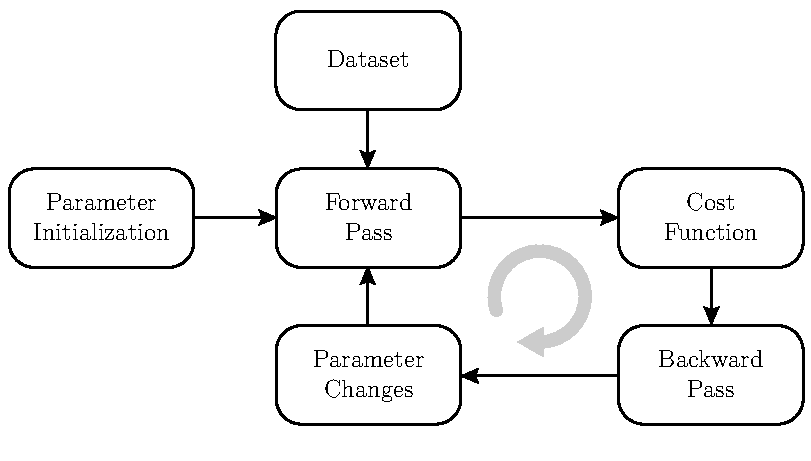
\includegraphics{images/training.pdf}
	\caption[Training Process]{Training Process}
	\label{fig:training}
\end{figure}

\subsubsection{Dataset Generation}
\label{sec:dataset-generation}
The whole training process is based on the dataset from which the network learns the correlations of input and label.
Usually, a dataset consists of input-label pairs, where the input is the data that is fed into the network and the label is the ground-truth.
In the case of a classification task, the label represents the category.
However, there is no general rule for the amount of data.
It can be said, that more data is better for generalization, but too many samples can lead to overfit the network to the shown data.
The latter means, that the network is trained to long or to intensive on the shown data.
The consequence is, that it adjusts its weights and biases to classify this data perfectly, but cannot reliably classify general, unknown data of same objects anymore, because they slightly differ.
Basically, the amount of data depends on the objective of the network.
For classifying whether an image is black or white, only a few training samples would be needed.
Is the objective classifying objects within images, it depends on the number of possible objects and their complexity.
If the objects are simple geometric shapes, then not as many samples are needed as if the objects are common objects like type of animals or cars.
For the latter the number of samples would probably be approximately 1000 examples per class.
Luckily, there are several datasets available, that are already sorted and labeled, like the MNIST handwritten digits or the ImageNet dataset.
Available datasets are not limited to images, but can contain CAD models like the ModelNet dataset which is used for this network architecture.

Samples of a dataset are split into a training and testing set, and sometimes a validation set\cite{James2014}.
The first contains data, the network trains on.
From this data correlations of input and label are found.
After arbitrary training steps where parameter changes happened, the performance of the network is tested on the validation set.
This is data, the network is not trained on.
The objective is to check if overfitting occurs.
If the accuracy of the training set increases, the accuracy of the validation set has to increase as well.
This shows that the network still learns and gets better.
If the accuracy of the training set increases, but the accuracy of the validation set stays the same or decreases, it is an indicator for overfitting.
The testing set is data the network is not trained on as well.
It serves as a final performance check of the network to confirm its general accuracy.
If no validation set is available, the testing set can be used.
How the dataset is split depends again on the number and complexity of samples and the objective.
However, a equal distribution of samples in each set should be minded.
Otherwise the performance will not be satisfying.
This means, if the network trains mostly on sweatshirts a test set with mostly pants would not yield an acceptable accuracy, because the network does not know these particular features.

For processing the dataset, a one-hot encoding\cite{Harris2012} of the labels is recommended.
Usually, the labels are categorical data.
This means, they contain label or string values, respectively, instead of numeric values, that the networks needs.
For example, there is a fashion variable with the values "boot", "sweatshirt" and "pants".
The network would not know how to interpret these.
Thus, these values need to be converted to numeric values.
Furthermore, if these label values are outputs of the network, it should be easily possible to convert them back from numeric values.
Hence, they are converted to integers that represent a category.
Referring to the example, this results in the numeric values 0, 1 and 2 for the labels "boot", "sweatshirt" and "pants", respectively.
But numeric values have a natural ordered relationship between each other, that neural networks could exploit.
The index of "pants" is higher than the one of "boot", but neither of these categories is better or worse than the other.
Therefore, the indices are one-hot encoded as well.
This means removing the integer representation and inserting binary variables for simulating existing features.
Applying this to the example results in the feature label vector $\vec{f}_1 = (0, 1, 0)^T$ for the "sweatshirt" label.
This vector has a length of the number of different categories available, where every element is 0 except the one of the corresponding category which is 1.
\tabref{tab:one-hot-encoding} summarizes this approach.
\begin{table}[]
	\caption[One-Hot Encoding of Categorical Data]{One-hot encoding of categorical data. First, categorical label values are transformed to numeric values representing a category index. Then, this is replaced with binary variables to represent features, that removes the natural relationship of numeric values to each other. This vector has a length of the number of different categories, where every element is 0 except for the corresponding category which is 1.}
	\label{tab:one-hot-encoding}
	\centering
	\begin{tabular}{l|l|l}
		Categorical   & Integer & One-Hot                   \\ \hline
		"Boot"       & 0       & $\vec{f}_0 = (1, 0, 0)^T$ \\
		"Sweatshirt" & 1       & $\vec{f}_1 = (0,1, 0)^T$  \\
		"Pants"      & 2       & $\vec{f}_2 = (0, 0, 1)^T$
	\end{tabular}
\end{table}
\subsubsection{Weight Initialization}
\label{sec:training-weight-initialization}
Before the actual training starts, the parameters, the weights and biases, of the network need to be initialized.
If this is done right, i.e. the values are in a range that supports training, optimization will be achieved in lesser or least time.
In the other case, a converging to optimal values can be impossible.
Reasons for this are the exploding or vanishing of gradients during backpropagation\cite{Hochreiter1991}.
In the backward-pass the gradients are computed for every layer and are passed from end to beginning using the chain rule.
For example, the derivative of the sigmoid function as it can be seen in \figref{fig:sigmoid-derivative} is in the range of $(0, 0.25]$.
If this is multiplied several times, the gradients at the beginning are way smaller than at the end.
If the weights are too small or too large, this effect is intensified.
This is partly true for other activation functions like the ReLU as well.
But here the gradients can become very large too, if the weights are really large.
None of these scenarios is desirable, because the optimal weights are either not reached or skipped.
\begin{figure}
	\setlength\figureheight{.4\textwidth}
	\setlength\figurewidth{.7\textwidth}
	\centering
	% This file was created by matplotlib2tikz v0.7.3.
\begin{tikzpicture}

\begin{axis}[
height=\figureheight,
legend cell align={left},
legend style={at={(0.03,0.97)}, anchor=north west, draw=white!80.0!black},
tick align=outside,
tick pos=left,
width=\figurewidth,
x grid style={white!90.01960784313725!black},
xlabel={x},
xmajorgrids,
xmin=-10.9995, xmax=10.9894999999996,
xtick style={color=black},
y grid style={white!90.01960784313725!black},
ylabel={y},
ymajorgrids,
ymin=-0.0499500416966799, ymax=1.04994958340047,
ytick style={color=black},
ytick={-0.2,0,0.2,0.4,0.6,0.8,1,1.2},
yticklabels={,0.0,0.2,0.4,0.6,0.8,1.0,}
]
\addplot [semithick, green!50.0!black]
table {%
-10 4.53978687024344e-05
-9.99 4.58541039469413e-05
-9.98 4.63149240092682e-05
-9.97 4.67803749590633e-05
-9.96 4.72505033288101e-05
-9.95 4.77253561184756e-05
-9.94 4.82049808002045e-05
-9.93 4.86894253230617e-05
-9.92 4.91787381178213e-05
-9.91 4.96729681018042e-05
-9.9 5.01721646837641e-05
-9.89 5.06763777688226e-05
-9.88 5.11856577634538e-05
-9.87 5.17000555805188e-05
-9.86 5.22196226443509e-05
-9.85 5.27444108958916e-05
-9.84 5.32744727978785e-05
-9.83 5.38098613400846e-05
-9.82 5.43506300446111e-05
-9.81 5.48968329712322e-05
-9.8 5.54485247227947e-05
-9.79 5.60057604506708e-05
-9.78 5.65685958602659e-05
-9.77 5.71370872165821e-05
-9.76000000000001 5.77112913498368e-05
-9.75000000000001 5.82912656611383e-05
-9.74000000000001 5.88770681282178e-05
-9.73000000000001 5.94687573112193e-05
-9.72000000000001 6.00663923585472e-05
-9.71000000000001 6.06700330127733e-05
-9.70000000000001 6.1279739616602e-05
-9.69000000000001 6.18955731188962e-05
-9.68000000000001 6.2517595080763e-05
-9.67000000000001 6.31458676817011e-05
-9.66000000000001 6.37804537258095e-05
-9.65000000000001 6.44214166480583e-05
-9.64000000000001 6.50688205206224e-05
-9.63000000000001 6.57227300592795e-05
-9.62000000000001 6.63832106298714e-05
-9.61000000000001 6.705032825483e-05
-9.60000000000001 6.77241496197696e-05
-9.59000000000001 6.84047420801449e-05
-9.58000000000001 6.90921736679753e-05
-9.57000000000001 6.97865130986373e-05
-9.56000000000001 7.04878297777246e-05
-9.55000000000001 7.11961938079774e-05
-9.54000000000001 7.19116759962808e-05
-9.53000000000001 7.26343478607335e-05
-9.52000000000001 7.33642816377872e-05
-9.51000000000001 7.41015502894582e-05
-9.50000000000001 7.48462275106104e-05
-9.49000000000001 7.55983877363123e-05
-9.48000000000001 7.63581061492668e-05
-9.47000000000001 7.71254586873163e-05
-9.46000000000001 7.79005220510224e-05
-9.45000000000001 7.86833737113223e-05
-9.44000000000001 7.9474091917261e-05
-9.43000000000001 8.02727557038022e-05
-9.42000000000001 8.10794448997163e-05
-9.41000000000001 8.18942401355483e-05
-9.40000000000001 8.27172228516654e-05
-9.39000000000001 8.35484753063848e-05
-9.38000000000001 8.4388080584184e-05
-9.37000000000001 8.5236122603992e-05
-9.36000000000001 8.60926861275648e-05
-9.35000000000001 8.69578567679443e-05
-9.34000000000001 8.78317209980021e-05
-9.33000000000001 8.87143661590688e-05
-9.32000000000001 8.96058804696499e-05
-9.31000000000001 9.05063530342293e-05
-9.30000000000001 9.14158738521601e-05
-9.29000000000002 9.23345338266462e-05
-9.28000000000002 9.32624247738116e-05
-9.27000000000002 9.4199639431863e-05
-9.26000000000002 9.51462714703421e-05
-9.25000000000002 9.61024154994724e-05
-9.24000000000002 9.70681670795981e-05
-9.23000000000002 9.80436227307186e-05
-9.22000000000002 9.90288799421182e-05
-9.21000000000002 0.000100024037182092
-9.20000000000002 0.000101029193907771
-9.19000000000002 0.000102044450575041
-9.18000000000002 0.000103069908648568
-9.17000000000002 0.000104105670611915
-9.16000000000002 0.000105151839977772
-9.15000000000002 0.000106208521298275
-9.14000000000002 0.000107275820175438
-9.13000000000002 0.000108353843271689
-9.12000000000002 0.000109442698320503
-9.11000000000002 0.000110542494137153
-9.10000000000002 0.000111653340629561
-9.09000000000002 0.000112775348809258
-9.08000000000002 0.00011390863080246
-9.07000000000002 0.000115053299861247
-9.06000000000002 0.000116209470374859
-9.05000000000002 0.000117377257881102
-9.04000000000002 0.000118556779077874
-9.03000000000002 0.000119748151834796
-9.02000000000002 0.00012095149520497
-9.01000000000002 0.000122166929436849
-9.00000000000002 0.000123394575986229
-8.99000000000002 0.000124634557528356
-8.98000000000002 0.000125886997970159
-8.97000000000002 0.000127152022462606
-8.96000000000002 0.000128429757413177
-8.95000000000002 0.000129720330498472
-8.94000000000002 0.000131023870676934
-8.93000000000002 0.00013234050820171
-8.92000000000002 0.000133670374633632
-8.91000000000002 0.000135013602854333
-8.90000000000002 0.000136370327079494
-8.89000000000002 0.00013774068287222
-8.88000000000002 0.000139124807156555
-8.87000000000002 0.000140522838231126
-8.86000000000002 0.000141934915782931
-8.85000000000002 0.000143361180901257
-8.84000000000002 0.000144801776091746
-8.83000000000002 0.000146256845290592
-8.82000000000003 0.000147726533878887
-8.81000000000003 0.000149210988697109
-8.80000000000003 0.000150710358059754
-8.79000000000003 0.000152224791770114
-8.78000000000003 0.000153754441135206
-8.77000000000003 0.000155299458980844
-8.76000000000003 0.000156859999666868
-8.75000000000003 0.000158436219102522
-8.74000000000003 0.000160028274761988
-8.73000000000003 0.000161636325700073
-8.72000000000003 0.000163260532568052
-8.71000000000003 0.000164901057629677
-8.70000000000003 0.000166558064777331
-8.69000000000003 0.000168231719548363
-8.68000000000003 0.000169922189141569
-8.67000000000003 0.000171629642433847
-8.66000000000003 0.000173354249997016
-8.65000000000003 0.000175096184114805
-8.64000000000003 0.000176855618800008
-8.63000000000003 0.000178632729811813
-8.62000000000003 0.000180427694673307
-8.61000000000003 0.000182240692689147
-8.60000000000003 0.000184071904963418
-8.59000000000003 0.000185921514417664
-8.58000000000003 0.000187789705809097
-8.57000000000003 0.000189676665748995
-8.56000000000003 0.000191582582721276
-8.55000000000003 0.000193507647101265
-8.54000000000003 0.000195452051174638
-8.53000000000003 0.000197415989156572
-8.52000000000003 0.000199399657211064
-8.51000000000003 0.000201403253470467
-8.50000000000003 0.0002034269780552
-8.49000000000003 0.000205471033093667
-8.48000000000003 0.000207535622742374
-8.47000000000003 0.000209620953206242
-8.46000000000003 0.000211727232759125
-8.45000000000003 0.000213854671764536
-8.44000000000003 0.000216003482696574
-8.43000000000003 0.000218173880161067
-8.42000000000003 0.000220366080916919
-8.41000000000003 0.000222580303897672
-8.40000000000003 0.000224816770233288
-8.39000000000003 0.000227075703272142
-8.38000000000003 0.000229357328603239
-8.37000000000003 0.000231661874078649
-8.36000000000003 0.000233989569836168
-8.35000000000004 0.000236340648322206
-8.34000000000004 0.000238715344314899
-8.33000000000004 0.000241113894947457
-8.32000000000004 0.000243536539731744
-8.31000000000004 0.000245983520582085
-8.30000000000004 0.000248455081839325
-8.29000000000004 0.000250951470295114
-8.28000000000004 0.000253472935216442
-8.27000000000004 0.000256019728370415
-8.26000000000004 0.000258592104049282
-8.25000000000004 0.00026119031909571
-8.24000000000004 0.000263814632928303
-8.23000000000004 0.000266465307567389
-8.22000000000004 0.000269142607661057
-8.21000000000004 0.000271846800511449
-8.20000000000004 0.000274578156101322
-8.19000000000004 0.000277336947120871
-8.18000000000004 0.000280123448994817
-8.17000000000004 0.000282937939909772
-8.16000000000004 0.000285780700841868
-8.15000000000004 0.000288652015584664
-8.14000000000004 0.000291552170777337
-8.13000000000004 0.000294481455933143
-8.12000000000004 0.000297440163468171
-8.11000000000004 0.000300428588730376
-8.10000000000004 0.000303447030028907
-8.09000000000004 0.000306495788663722
-8.08000000000004 0.000309575168955503
-8.07000000000004 0.000312685478275861
-8.06000000000004 0.00031582702707785
-8.05000000000004 0.000319000128926778
-8.04000000000004 0.00032220510053133
-8.03000000000004 0.000325442261774996
-8.02000000000004 0.000328711935747814
-8.01000000000004 0.000332014448778428
-8.00000000000004 0.000335350130466464
-7.99000000000004 0.000338719313715231
-7.98000000000004 0.000342122334764745
-7.97000000000004 0.000345559533225079
-7.96000000000004 0.000349031252110046
-7.95000000000004 0.000352537837871223
-7.94000000000004 0.000356079640432303
-7.93000000000004 0.000359657013223794
-7.92000000000004 0.000363270313218062
-7.91000000000004 0.000366919900964721
-7.90000000000004 0.00037060614062638
-7.89000000000004 0.000374329400014733
-7.88000000000005 0.000378090050627021
-7.87000000000005 0.000381888467682847
-7.86000000000005 0.00038572503016136
-7.85000000000005 0.000389600120838808
-7.84000000000005 0.000393514126326465
-7.83000000000005 0.000397467437108928
-7.82000000000005 0.000401460447582802
-7.81000000000005 0.000405493556095768
-7.80000000000005 0.000409567164986031
-7.79000000000005 0.000413681680622168
-7.78000000000005 0.000417837513443365
-7.77000000000005 0.00042203507800006
-7.76000000000005 0.00042627479299498
-7.75000000000005 0.000430557081324594
-7.74000000000005 0.000434882370120969
-7.73000000000005 0.000439251090794044
-7.72000000000005 0.000443663679074329
-7.71000000000005 0.000448120575056012
-7.70000000000005 0.000452622223240513
-7.69000000000005 0.000457169072580449
-7.68000000000005 0.000461761576524052
-7.67000000000005 0.000466400193060015
-7.66000000000005 0.000471085384762786
-7.65000000000005 0.000475817618838312
-7.64000000000005 0.000480597367170237
-7.63000000000005 0.000485425106366547
-7.62000000000005 0.000490301317806692
-7.61000000000005 0.000495226487689162
-7.60000000000005 0.000500201107079539
-7.59000000000005 0.000505225671959023
-7.58000000000005 0.000510300683273438
-7.57000000000005 0.000515426646982725
-7.56000000000005 0.000520604074110915
-7.55000000000005 0.000525833480796612
-7.54000000000005 0.000531115388343959
-7.53000000000005 0.000536450323274114
-7.52000000000005 0.000541838817377241
-7.51000000000005 0.000547281407765
-7.50000000000005 0.00055277863692357
-7.49000000000005 0.000558331052767186
-7.48000000000005 0.000563939208692207
-7.47000000000005 0.000569603663631721
-7.46000000000005 0.000575324982110682
-7.45000000000005 0.0005811037343016
-7.44000000000005 0.000586940496080771
-7.43000000000005 0.000592835849085066
-7.42000000000005 0.000598790380769285
-7.41000000000006 0.000604804684464065
-7.40000000000006 0.000610879359434367
-7.39000000000006 0.000617015010938541
-7.38000000000006 0.000623212250287964
-7.37000000000006 0.000629471694907274
-7.36000000000006 0.000635793968395193
-7.35000000000006 0.000642179700585949
-7.34000000000006 0.000648629527611308
-7.33000000000006 0.000655144091963206
-7.32000000000006 0.000661724042557007
-7.31000000000006 0.000668370034795379
-7.30000000000006 0.000675082730632799
-7.29000000000006 0.000681862798640694
-7.28000000000006 0.000688710914073216
-7.27000000000006 0.000695627758933676
-7.26000000000006 0.000702614022041614
-7.25000000000006 0.000709670399100547
-7.24000000000006 0.000716797592766362
-7.23000000000006 0.000723996312716402
-7.22000000000006 0.00073126727571921
-7.21000000000006 0.000738611205704974
-7.20000000000006 0.000746028833836653
-7.19000000000006 0.000753520898581804
-7.18000000000006 0.000761088145785115
-7.17000000000006 0.000768731328741647
-7.16000000000006 0.000776451208270797
-7.15000000000006 0.000784248552790979
-7.14000000000006 0.000792124138395046
-7.13000000000006 0.000800078748926446
-7.12000000000006 0.000808113176056122
-7.11000000000006 0.000816228219360168
-7.10000000000006 0.000824424686398244
-7.09000000000006 0.000832703392792759
-7.08000000000006 0.000841065162308828
-7.07000000000006 0.000849510826935011
-7.06000000000006 0.000858041226964839
-7.05000000000006 0.000866657211079143
-7.04000000000006 0.000875359636429182
-7.03000000000006 0.000884149368720584
-7.02000000000006 0.000893027282298109
-7.01000000000006 0.000901994260231235
-7.00000000000006 0.000911051194400587
-6.99000000000006 0.000920198985585201
-6.98000000000006 0.000929438543550642
-6.97000000000006 0.000938770787137987
-6.96000000000006 0.000948196644353664
-6.95000000000007 0.000957717052460177
-6.94000000000007 0.00096733295806771
-6.93000000000007 0.000977045317226621
-6.92000000000007 0.000986855095520843
-6.91000000000007 0.000996763268162188
-6.90000000000007 0.00100677082008557
-6.89000000000007 0.00101687874604516
-6.88000000000007 0.00102708805071145
-6.87000000000007 0.00103739974876932
-6.86000000000007 0.00104781486501699
-6.85000000000007 0.00105833443446594
-6.84000000000007 0.00106895950244189
-6.83000000000007 0.00107969112468662
-6.82000000000007 0.0010905303674609
-6.81000000000007 0.00110147830764833
-6.80000000000007 0.00111253603286025
-6.79000000000007 0.00112370464154163
-6.78000000000007 0.00113498524307802
-6.77000000000007 0.00114637895790346
-6.76000000000007 0.00115788691760954
-6.75000000000007 0.00116951026505543
-6.74000000000007 0.00118125015447904
-6.73000000000007 0.00119310775160918
-6.72000000000007 0.00120508423377886
-6.71000000000007 0.00121718079003969
-6.70000000000007 0.00122939862127733
-6.69000000000007 0.00124173894032813
-6.68000000000007 0.0012542029720968
-6.67000000000007 0.00126679195367532
-6.66000000000007 0.00127950713446292
-6.65000000000007 0.00129234977628725
-6.64000000000007 0.00130532115352668
-6.63000000000007 0.00131842255323385
-6.62000000000007 0.00133165527526034
-6.61000000000007 0.00134502063238256
-6.60000000000007 0.00135851995042886
-6.59000000000007 0.00137215456840785
-6.58000000000007 0.00138592583863798
-6.57000000000007 0.0013998351268783
-6.56000000000007 0.00141388381246055
-6.55000000000007 0.00142807328842247
-6.54000000000007 0.00144240496164241
-6.53000000000007 0.00145688025297522
-6.52000000000007 0.00147150059738942
-6.51000000000007 0.00148626744410572
-6.50000000000007 0.00150118225673688
-6.49000000000007 0.00151624651342882
-6.48000000000008 0.00153146170700317
-6.47000000000008 0.00154682934510116
-6.46000000000008 0.00156235095032884
-6.45000000000008 0.00157802806040374
-6.44000000000008 0.00159386222830289
-6.43000000000008 0.00160985502241227
-6.42000000000008 0.00162600802667769
-6.41000000000008 0.00164232284075709
-6.40000000000008 0.00165880108017429
-6.39000000000008 0.00167544437647422
-6.38000000000008 0.00169225437737958
-6.37000000000008 0.00170923274694906
-6.36000000000008 0.00172638116573702
-6.35000000000008 0.00174370133095464
-6.34000000000008 0.00176119495663271
-6.33000000000008 0.00177886377378583
-6.32000000000008 0.0017967095305783
-6.31000000000008 0.00181473399249146
-6.30000000000008 0.00183293894249266
-6.29000000000008 0.00185132618120589
-6.28000000000008 0.0018698975270839
-6.27000000000008 0.00188865481658203
-6.26000000000008 0.00190759990433367
-6.25000000000008 0.00192673466332732
-6.24000000000008 0.0019460609850854
-6.23000000000008 0.00196558077984468
-6.22000000000008 0.00198529597673842
-6.21000000000008 0.00200520852398024
-6.20000000000008 0.00202532038904972
-6.19000000000008 0.00204563355887968
-6.18000000000008 0.00206615004004532
-6.17000000000008 0.00208687185895503
-6.16000000000008 0.00210780106204308
-6.15000000000008 0.00212893971596402
-6.14000000000008 0.00215028990778896
-6.13000000000008 0.00217185374520368
-6.12000000000008 0.00219363335670856
-6.11000000000008 0.00221563089182042
-6.10000000000008 0.00223784852127615
-6.09000000000008 0.00226028843723836
-6.08000000000008 0.00228295285350287
-6.07000000000008 0.00230584400570812
-6.06000000000008 0.00232896415154654
-6.05000000000008 0.00235231557097795
-6.04000000000008 0.00237590056644479
-6.03000000000008 0.00239972146308948
-6.02000000000008 0.00242378060897376
-6.01000000000009 0.00244808037529998
-6.00000000000009 0.00247262315663456
-5.99000000000009 0.00249741137113341
-5.98000000000009 0.00252244746076948
-5.97000000000009 0.00254773389156238
-5.96000000000009 0.00257327315381015
-5.95000000000009 0.00259906776232312
-5.94000000000009 0.00262512025665997
-5.93000000000009 0.00265143320136586
-5.92000000000009 0.00267800918621288
-5.91000000000009 0.00270485082644259
-5.90000000000009 0.00273196076301082
-5.89000000000009 0.00275934166283472
-5.88000000000009 0.00278699621904204
-5.87000000000009 0.00281492715122271
-5.86000000000009 0.00284313720568269
-5.85000000000009 0.00287162915570015
-5.84000000000009 0.00290040580178394
-5.83000000000009 0.00292946997193449
-5.82000000000009 0.00295882452190697
-5.81000000000009 0.00298847233547689
-5.80000000000009 0.00301841632470815
-5.79000000000009 0.00304865943022343
-5.78000000000009 0.00307920462147702
-5.77000000000009 0.00311005489703024
-5.76000000000009 0.00314121328482914
-5.75000000000009 0.0031726828424849
-5.74000000000009 0.00320446665755659
-5.73000000000009 0.00323656784783655
-5.72000000000009 0.00326898956163832
-5.71000000000009 0.00330173497808715
-5.70000000000009 0.00333480730741304
-5.69000000000009 0.00336820979124652
-5.68000000000009 0.00340194570291695
-5.67000000000009 0.00343601834775354
-5.66000000000009 0.00347043106338901
-5.65000000000009 0.00350518722006602
-5.64000000000009 0.00354029022094618
-5.63000000000009 0.00357574350242196
-5.62000000000009 0.00361155053443121
-5.61000000000009 0.00364771482077459
-5.60000000000009 0.00368423989943564
-5.59000000000009 0.00372112934290386
-5.58000000000009 0.00375838675850045
-5.57000000000009 0.003796015788707
-5.56000000000009 0.00383402011149708
-5.55000000000009 0.00387240344067067
-5.5400000000001 0.0039111695261915
-5.5300000000001 0.00395032215452744
-5.5200000000001 0.00398986514899372
-5.5100000000001 0.00402980237009923
-5.5000000000001 0.00407013771589574
-5.4900000000001 0.00411087512233024
-5.4800000000001 0.00415201856360025
-5.4700000000001 0.00419357205251221
-5.4600000000001 0.00423553964084302
-5.4500000000001 0.00427792541970456
-5.4400000000001 0.0043207335199115
-5.4300000000001 0.00436396811235212
-5.4200000000001 0.00440763340836238
-5.4100000000001 0.00445173366010317
-5.4000000000001 0.00449627316094074
-5.3900000000001 0.00454125624583043
-5.3800000000001 0.00458668729170357
-5.3700000000001 0.00463257071785773
-5.3600000000001 0.00467891098635024
-5.3500000000001 0.00472571260239501
-5.3400000000001 0.00477298011476273
-5.3300000000001 0.00482071811618437
-5.3200000000001 0.00486893124375816
-5.3100000000001 0.00491762417935984
-5.3000000000001 0.00496680165005647
-5.2900000000001 0.00501646842852355
-5.2800000000001 0.00506662933346575
-5.2700000000001 0.00511728923004097
-5.2600000000001 0.00516845303028805
-5.2500000000001 0.00522012569355787
-5.2400000000001 0.00527231222694814
-5.2300000000001 0.00532501768574163
-5.2200000000001 0.00537824717384806
-5.2100000000001 0.00543200584424957
-5.2000000000001 0.00548629889944985
-5.1900000000001 0.00554113159192684
-5.1800000000001 0.00559650922458923
-5.1700000000001 0.0056524371512365
-5.1600000000001 0.00570892077702276
-5.1500000000001 0.00576596555892431
-5.1400000000001 0.00582357700621092
-5.1300000000001 0.00588176068092085
-5.1200000000001 0.00594052219833976
-5.1100000000001 0.00599986722748326
-5.1000000000001 0.00605980149158349
-5.0900000000001 0.00612033076857929
-5.0800000000001 0.0061814608916105
-5.07000000000011 0.0062431977495159
-5.06000000000011 0.0063055472873352
-5.05000000000011 0.00636851550681488
-5.04000000000011 0.00643210846691796
-5.03000000000011 0.00649633228433775
-5.02000000000011 0.00656119313401553
-5.01000000000011 0.00662669724966224
-5.00000000000011 0.00669285092428415
-4.99000000000011 0.00675966051071253
-4.98000000000011 0.00682713242213744
-4.97000000000011 0.00689527313264541
-4.96000000000011 0.00696408917776135
-4.95000000000011 0.00703358715499441
-4.94000000000011 0.00710377372438802
-4.93000000000011 0.00717465560907397
-4.92000000000011 0.00724623959583065
-4.91000000000011 0.00731853253564544
-4.90000000000011 0.00739154134428118
-4.89000000000011 0.00746527300284688
-4.88000000000011 0.00753973455837258
-4.87000000000011 0.00761493312438833
-4.86000000000011 0.0076908758815075
-4.85000000000011 0.00776757007801415
-4.84000000000011 0.00784502303045478
-4.83000000000011 0.00792324212423412
-4.82000000000011 0.00800223481421537
-4.81000000000011 0.00808200862532451
-4.80000000000011 0.008162571153159
-4.79000000000011 0.00824393006460066
-4.78000000000011 0.00832609309843287
-4.77000000000011 0.00840906806596205
-4.76000000000011 0.00849286285164341
-4.75000000000011 0.00857748541371103
-4.74000000000011 0.0086629437848122
-4.73000000000011 0.00874924607264609
-4.72000000000011 0.00883640046060673
-4.71000000000011 0.00892441520843032
-4.70000000000011 0.00901329865284682
-4.69000000000011 0.00910305920823586
-4.68000000000011 0.00919370536728706
-4.67000000000011 0.00928524570166453
-4.66000000000011 0.0093776888626758
-4.65000000000011 0.00947104358194504
-4.64000000000011 0.00956531867209059
-4.63000000000011 0.00966052302740681
-4.62000000000011 0.00975666562455025
-4.61000000000011 0.00985375552323015
-4.60000000000012 0.00995180186690319
-4.59000000000012 0.0100508138834726
-4.58000000000012 0.0101508008859916
-4.57000000000012 0.0102517722733708
-4.56000000000012 0.0103537375310906
-4.55000000000012 0.0104567062319169
-4.54000000000012 0.0105606880366219
-4.53000000000012 0.0106656926947088
-4.52000000000012 0.0107717300451404
-4.51000000000012 0.0108788100170727
-4.50000000000012 0.0109869426305919
-4.49000000000012 0.0110961379974563
-4.48000000000012 0.0112064063218416
-4.47000000000012 0.011317757901091
-4.46000000000012 0.0114302031264694
-4.45000000000012 0.0115437524839209
-4.44000000000012 0.0116584165548317
-4.43000000000012 0.0117742060167958
-4.42000000000012 0.0118911316443856
-4.41000000000012 0.012009204309926
-4.40000000000012 0.0121284349842728
-4.39000000000012 0.0122488347375951
-4.38000000000012 0.012370414740161
-4.37000000000012 0.0124931862631281
-4.36000000000012 0.0126171606793372
-4.35000000000012 0.0127423494641101
-4.34000000000012 0.012868764196051
-4.33000000000012 0.0129964165578518
-4.32000000000012 0.0131253183371012
-4.31000000000012 0.0132554814270972
-4.30000000000012 0.0133869178276632
-4.29000000000012 0.013519639645968
-4.28000000000012 0.0136536590973492
-4.27000000000012 0.0137889885061399
-4.26000000000012 0.0139256403064987
-4.25000000000012 0.0140636270432438
-4.24000000000012 0.0142029613726894
-4.23000000000012 0.0143436560634864
-4.22000000000012 0.0144857239974651
-4.21000000000012 0.0146291781704825
-4.20000000000012 0.0147740316932713
-4.19000000000012 0.0149202977922924
-4.18000000000012 0.015067989810591
-4.17000000000012 0.0152171212086544
-4.16000000000012 0.0153677055652737
-4.15000000000012 0.015519756578407
-4.14000000000012 0.0156732880660466
-4.13000000000013 0.0158283139670879
-4.12000000000013 0.0159848483422006
-4.11000000000013 0.0161429053747032
-4.10000000000013 0.0163024993714389
-4.09000000000013 0.0164636447636542
-4.08000000000013 0.0166263561078796
-4.07000000000013 0.0167906480868117
-4.06000000000013 0.0169565355101987
-4.05000000000013 0.0171240333157256
-4.04000000000013 0.0172931565699033
-4.03000000000013 0.0174639204689575
-4.02000000000013 0.0176363403397205
-4.01000000000013 0.0178104316405232
-4.00000000000013 0.0179862099620893
-3.99000000000013 0.0181636910284302
-3.98000000000013 0.018342890697741
-3.97000000000013 0.0185238249632971
-3.96000000000013 0.0187065099543522
-3.95000000000013 0.0188909619370367
-3.94000000000013 0.0190771973152557
-3.93000000000013 0.0192652326315892
-3.92000000000013 0.0194550845681906
-3.91000000000013 0.0196467699476862
-3.90000000000013 0.019840305734075
-3.89000000000013 0.0200357090336271
-3.88000000000013 0.0202329970957828
-3.87000000000013 0.0204321873140504
-3.86000000000013 0.0206332972269036
-3.85000000000013 0.0208363445186778
-3.84000000000013 0.0210413470204656
-3.83000000000013 0.0212483227110108
-3.82000000000013 0.0214572897176008
-3.81000000000013 0.0216682663169577
-3.80000000000013 0.0218812709361276
-3.79000000000013 0.0220963221533673
-3.78000000000013 0.0223134386990293
-3.77000000000013 0.0225326394564444
-3.76000000000013 0.022753943462801
-3.75000000000013 0.0229773699100226
-3.74000000000013 0.0232029381456411
-3.73000000000013 0.0234306676736673
-3.72000000000013 0.0236605781554581
-3.71000000000013 0.0238926894105796
-3.70000000000013 0.024127021417666
-3.69000000000013 0.0243635943152746
-3.68000000000013 0.0246024284027362
-3.67000000000013 0.0248435441410004
-3.66000000000014 0.0250869621534765
-3.65000000000014 0.0253327032268684
-3.64000000000014 0.0255807883120043
-3.63000000000014 0.0258312385246606
-3.62000000000014 0.0260840751463795
-3.61000000000014 0.0263393196252799
-3.60000000000014 0.0265969935768623
-3.59000000000014 0.0268571187848061
-3.58000000000014 0.0271197172017594
-3.57000000000014 0.027384810950122
-3.56000000000014 0.0276524223228194
-3.55000000000014 0.0279225737840693
-3.54000000000014 0.0281952879701388
-3.53000000000014 0.0284705876900934
-3.52000000000014 0.0287484959265361
-3.51000000000014 0.0290290358363369
-3.50000000000014 0.0293122307513524
-3.49000000000014 0.0295981041791352
-3.48000000000014 0.0298866798036322
-3.47000000000014 0.0301779814858719
-3.46000000000014 0.03047203326464
-3.45000000000014 0.0307688593571438
-3.44000000000014 0.0310684841596632
-3.43000000000014 0.0313709322481897
-3.42000000000014 0.0316762283790521
-3.41000000000014 0.0319843974895289
-3.40000000000014 0.0322954646984461
-3.39000000000014 0.0326094553067611
-3.38000000000014 0.0329263947981318
-3.37000000000014 0.0332463088394696
-3.36000000000014 0.0335692232814779
-3.35000000000014 0.0338951641591735
-3.34000000000014 0.0342241576923912
-3.33000000000014 0.0345562302862718
-3.32000000000014 0.034891408531732
-3.31000000000014 0.0352297192059166
-3.30000000000014 0.0355711892726313
-3.29000000000014 0.0359158458827568
-3.28000000000014 0.0362637163746433
-3.27000000000014 0.0366148282744848
-3.26000000000014 0.0369692092966719
-3.25000000000014 0.0373268873441243
-3.24000000000014 0.0376878905086007
-3.23000000000014 0.0380522470709868
-3.22000000000014 0.03841998550156
-3.21000000000014 0.0387911344602306
-3.20000000000014 0.0391657227967589
-3.19000000000015 0.0395437795509474
-3.18000000000015 0.0399253339528082
-3.17000000000015 0.0403104154227036
-3.16000000000015 0.0406990535714608
-3.15000000000015 0.0410912782004593
-3.14000000000015 0.04148711930169
-3.13000000000015 0.0418866070577868
-3.12000000000015 0.0422897718420279
-3.11000000000015 0.0426966442183079
-3.10000000000015 0.0431072549410801
-3.09000000000015 0.0435216349552661
-3.08000000000015 0.0439398153961351
-3.07000000000015 0.0443618275891501
-3.06000000000015 0.0447877030497804
-3.05000000000015 0.0452174734832811
-3.04000000000015 0.0456511707844373
-3.03000000000015 0.0460888270372731
-3.02000000000015 0.0465304745147249
-3.01000000000015 0.0469761456782769
-3.00000000000015 0.04742587317756
-2.99000000000015 0.0478796898499121
-2.98000000000015 0.0483376287198983
-2.97000000000015 0.048799722998793
-2.96000000000015 0.0492660060840196
-2.95000000000015 0.0497365115585496
-2.94000000000015 0.0502112731902594
-2.93000000000015 0.0506903249312434
-2.92000000000015 0.0511737009170843
-2.91000000000015 0.0516614354660774
-2.90000000000015 0.0521535630784103
-2.89000000000015 0.0526501184352954
-2.88000000000015 0.0531511363980561
-2.87000000000015 0.0536566520071642
-2.86000000000015 0.0541667004812283
-2.85000000000015 0.0546813172159329
-2.84000000000015 0.0552005377829263
-2.83000000000015 0.0557243979286574
-2.82000000000015 0.0562529335731592
-2.81000000000015 0.0567861808087803
-2.80000000000015 0.0573241758988604
-2.79000000000015 0.0578669552763526
-2.78000000000015 0.0584145555423878
-2.77000000000015 0.0589670134647832
-2.76000000000015 0.0595243659764929
-2.75000000000015 0.0600866501739989
-2.74000000000015 0.0606539033156433
-2.73000000000015 0.0612261628198991
-2.72000000000016 0.0618034662635796
-2.71000000000016 0.0623858513799853
-2.70000000000016 0.0629733560569873
-2.69000000000016 0.063566018335046
-2.68000000000016 0.0641638764051646
-2.67000000000016 0.0647669686067761
-2.66000000000016 0.0653753334255631
-2.65000000000016 0.0659890094912091
-2.64000000000016 0.0666080355750809
-2.63000000000016 0.0672324505878402
-2.62000000000016 0.0678622935769845
-2.61000000000016 0.068497603724316
-2.60000000000016 0.0691384203433367
-2.59000000000016 0.0697847828765698
-2.58000000000016 0.0704367308928067
-2.57000000000016 0.0710943040842767
-2.56000000000016 0.0717575422637408
-2.55000000000016 0.072426485361507
-2.54000000000016 0.0731011734223674
-2.53000000000016 0.0737816466024544
-2.52000000000016 0.0744679451660171
-2.51000000000016 0.0751601094821155
-2.50000000000016 0.0758581800212323
-2.49000000000016 0.0765621973518009
-2.48000000000016 0.0772722021366485
-2.47000000000016 0.0779882351293548
-2.46000000000016 0.0787103371705236
-2.45000000000016 0.0794385491839666
-2.44000000000016 0.0801729121728004
-2.43000000000016 0.0809134672154534
-2.42000000000016 0.0816602554615825
-2.41000000000016 0.0824133181279006
-2.40000000000016 0.08317269649391
-2.39000000000016 0.0839384318975457
-2.38000000000016 0.0847105657307232
-2.37000000000016 0.0854891394347938
-2.36000000000016 0.0862741944959039
-2.35000000000016 0.0870657724402583
-2.34000000000016 0.0878639148292882
-2.33000000000016 0.0886686632547201
-2.32000000000016 0.0894800593335481
-2.31000000000016 0.0902981447029064
-2.30000000000016 0.0911229610148425
-2.29000000000016 0.0919545499309906
-2.28000000000016 0.0927929531171432
-2.27000000000016 0.0936382122377217
-2.26000000000016 0.0944903689501452
-2.25000000000017 0.0953494648990953
-2.24000000000017 0.0962155417106785
-2.23000000000017 0.0970886409864844
-2.22000000000017 0.0979688042975393
-2.21000000000017 0.0988560731781546
-2.20000000000017 0.0997504891196702
-2.19000000000017 0.100652093564092
-2.18000000000017 0.101560927897621
-2.17000000000017 0.102477033444082
-2.16000000000017 0.103400451458234
-2.15000000000017 0.104331223118986
-2.14000000000017 0.105269389522494
-2.13000000000017 0.10621499167516
-2.12000000000017 0.107168070486512
-2.11000000000017 0.108128666761987
-2.10000000000017 0.109096821195597
-2.09000000000017 0.110072574362486
-2.08000000000017 0.111055966711391
-2.07000000000017 0.112047038556973
-2.06000000000017 0.113045830072062
-2.05000000000017 0.114052381279774
-2.04000000000017 0.115066732045533
-2.03000000000017 0.116088922068977
-2.02000000000017 0.117118990875763
-2.01000000000017 0.118156977809252
-2.00000000000017 0.1192029220221
-1.99000000000017 0.120256862467733
-1.98000000000017 0.121318837891719
-1.97000000000017 0.12238888682303
-1.96000000000017 0.123467047565205
-1.95000000000017 0.124553358187398
-1.94000000000017 0.125647856515327
-1.93000000000017 0.126750580122122
-1.92000000000017 0.127861566319062
-1.91000000000017 0.128980852146216
-1.90000000000017 0.130108474362978
-1.89000000000017 0.131244469438504
-1.88000000000017 0.132388873542046
-1.87000000000017 0.133541722533192
-1.86000000000017 0.134703051952008
-1.85000000000017 0.135872897009074
-1.84000000000017 0.137051292575439
-1.83000000000017 0.138238273172473
-1.82000000000017 0.139433872961629
-1.81000000000017 0.140638125734113
-1.80000000000017 0.141851064900467
-1.79000000000018 0.143072723480059
-1.78000000000018 0.144303134090497
-1.77000000000018 0.145542328936943
-1.76000000000018 0.14679033980136
-1.75000000000018 0.148047198031667
-1.74000000000018 0.149312934530821
-1.73000000000018 0.150587579745821
-1.72000000000018 0.151871163656637
-1.71000000000018 0.153163715765063
-1.70000000000018 0.154465265083512
-1.69000000000018 0.155775840123724
-1.68000000000018 0.157095468885429
-1.67000000000018 0.158424178844932
-1.66000000000018 0.159761996943645
-1.65000000000018 0.161108949576561
-1.64000000000018 0.162465062580672
-1.63000000000018 0.163830361223334
-1.62000000000018 0.16520487019059
-1.61000000000018 0.166588613575435
-1.60000000000018 0.167981614866051
-1.59000000000018 0.169383896933993
-1.58000000000018 0.170795482022349
-1.57000000000018 0.172216391733852
-1.56000000000018 0.173646647018979
-1.55000000000018 0.175086268164014
-1.54000000000018 0.176535274779091
-1.53000000000018 0.17799368578622
-1.52000000000018 0.1794615194073
-1.51000000000018 0.180938793152115
-1.50000000000018 0.182425523806329
-1.49000000000018 0.183921727419477
-1.48000000000018 0.185427419292955
-1.47000000000018 0.186942613968019
-1.46000000000018 0.188467325213792
-1.45000000000018 0.190001566015285
-1.44000000000018 0.191545348561439
-1.43000000000018 0.193098684233188
-1.42000000000018 0.194661583591549
-1.41000000000018 0.19623405636575
-1.40000000000018 0.197816111441389
-1.39000000000018 0.199407756848639
-1.38000000000018 0.2010089997505
-1.37000000000018 0.202619846431101
-1.36000000000018 0.204240302284062
-1.35000000000018 0.205870371800917
-1.34000000000018 0.207510058559605
-1.33000000000018 0.209159365213033
-1.32000000000019 0.210818293477716
-1.31000000000019 0.212486844122508
-1.30000000000019 0.21416501695741
-1.29000000000019 0.215852810822483
-1.28000000000019 0.217550223576856
-1.27000000000019 0.21925725208784
-1.26000000000019 0.220973892220156
-1.25000000000019 0.222700138825277
-1.24000000000019 0.224435985730894
-1.23000000000019 0.226181425730513
-1.22000000000019 0.227936450573183
-1.21000000000019 0.229701050953365
-1.20000000000019 0.231475216500949
-1.19000000000019 0.233258935771424
-1.18000000000019 0.235052196236201
-1.17000000000019 0.236854984273111
-1.16000000000019 0.238667285157055
-1.15000000000019 0.240489083050854
-1.14000000000019 0.24232036099626
-1.13000000000019 0.244161100905168
-1.12000000000019 0.246011283551017
-1.11000000000019 0.247870888560395
-1.10000000000019 0.249739894404847
-1.09000000000019 0.2516182783929
-1.08000000000019 0.253506016662302
-1.07000000000019 0.255403084172488
-1.06000000000019 0.257309454697278
-1.05000000000019 0.259225100817809
-1.04000000000019 0.261149993915714
-1.03000000000019 0.263084104166543
-1.02000000000019 0.265027400533444
-1.01000000000019 0.266979850761105
-1.00000000000019 0.268941421369957
-0.990000000000192 0.270912077650656
-0.980000000000192 0.272891783658832
-0.970000000000192 0.274880502210139
-0.960000000000193 0.276878194875572
-0.950000000000193 0.278884821977098
-0.940000000000193 0.280900342583577
-0.930000000000193 0.282924714506988
-0.920000000000194 0.284957894298971
-0.910000000000194 0.286999837247679
-0.900000000000194 0.289050497374956
-0.890000000000194 0.29110982743384
-0.880000000000194 0.293177778906392
-0.870000000000195 0.295254302001868
-0.860000000000195 0.297339345655228
-0.850000000000195 0.299432857525986
-0.840000000000195 0.30153478399742
-0.830000000000195 0.303645070176125
-0.820000000000196 0.305763659891928
-0.810000000000196 0.30789049569817
-0.800000000000196 0.310025518872346
-0.790000000000196 0.312168669417117
-0.780000000000197 0.314319886061704
-0.770000000000197 0.316479106263642
-0.760000000000197 0.318646266210932
-0.750000000000197 0.320821300824564
-0.740000000000197 0.323004143761434
-0.730000000000198 0.325194727417643
-0.720000000000198 0.327392982932196
-0.710000000000198 0.329598840191088
-0.700000000000198 0.33181222783179
-0.690000000000198 0.334033073248136
-0.680000000000199 0.336261302595603
-0.670000000000199 0.338496840797003
-0.660000000000199 0.34073961154857
-0.650000000000199 0.342989537326456
-0.6400000000002 0.345246539393636
-0.6300000000002 0.34751053780721
-0.6200000000002 0.349781451426127
-0.6100000000002 0.352059197919304
-0.6000000000002 0.354343693774159
-0.590000000000201 0.356634854305552
-0.580000000000201 0.358932593665137
-0.570000000000201 0.361236824851112
-0.560000000000201 0.363547459718387
-0.550000000000201 0.365864408989153
-0.540000000000202 0.368187582263851
-0.530000000000202 0.370516888032558
-0.520000000000202 0.372852233686757
-0.510000000000202 0.375193525531523
-0.500000000000203 0.377540668798098
-0.490000000000203 0.379893567656862
-0.480000000000203 0.382252125230703
-0.470000000000203 0.38461624360877
-0.460000000000203 0.386985823860616
-0.450000000000204 0.38936076605073
-0.440000000000204 0.391740969253437
-0.430000000000204 0.394126331568191
-0.420000000000204 0.396516750135225
-0.410000000000204 0.398912121151581
-0.400000000000205 0.401312339887499
-0.390000000000205 0.403717300703163
-0.380000000000205 0.406126897065808
-0.370000000000205 0.40854102156717
-0.360000000000205 0.410959565941285
-0.350000000000206 0.41338242108262
-0.340000000000206 0.415809477064543
-0.330000000000206 0.418240623158114
-0.320000000000206 0.4206757478512
-0.310000000000207 0.423114738867903
-0.300000000000207 0.42555748318829
-0.290000000000207 0.428003867068431
-0.280000000000207 0.43045377606072
-0.270000000000207 0.432907095034495
-0.260000000000208 0.43536370819692
-0.250000000000208 0.437823499114151
-0.240000000000208 0.440286350732756
-0.230000000000208 0.442752145401393
-0.220000000000208 0.445220764892734
-0.210000000000209 0.447692090425623
-0.200000000000209 0.45016600268747
-0.190000000000209 0.452642381856859
-0.180000000000209 0.455121107626368
-0.17000000000021 0.457602059225597
-0.16000000000021 0.460085115444382
-0.15000000000021 0.462570154656198
-0.14000000000021 0.465057054841733
-0.13000000000021 0.467545693612629
-0.120000000000211 0.470035948235376
-0.110000000000211 0.472527695655354
-0.100000000000211 0.475020812521007
-0.0900000000002112 0.477515175208147
-0.0800000000002115 0.480010659844365
-0.0700000000002117 0.482507142333557
-0.0600000000002119 0.485004498380537
-0.0500000000002121 0.487502603515737
-0.0400000000002123 0.490001333119982
-0.0300000000002125 0.492500562449326
-0.0200000000002127 0.495000166659947
-0.0100000000002129 0.497500020833072
-2.1316282072803e-13 0.499999999999947
0.00999999999978662 0.502499979166822
0.0199999999997864 0.504999833339946
0.0299999999997862 0.507499437550567
0.039999999999786 0.509998666879912
0.0499999999997858 0.512497396484157
0.0599999999997856 0.514995501619356
0.0699999999997853 0.517492857666336
0.0799999999997851 0.519989340155528
0.0899999999997849 0.522484824791747
0.0999999999997847 0.524979187478886
0.109999999999784 0.52747230434454
0.119999999999784 0.529964051764518
0.129999999999784 0.532454306387265
0.139999999999784 0.534942945158161
0.149999999999784 0.537429845343696
0.159999999999783 0.539914884555512
0.169999999999783 0.542397940774297
0.179999999999783 0.544878892373526
0.189999999999783 0.547357618143035
0.199999999999783 0.549833997312424
0.209999999999782 0.552307909574271
0.219999999999782 0.554779235107161
0.229999999999782 0.557247854598502
0.239999999999782 0.559713649267139
0.249999999999782 0.562176500885744
0.259999999999781 0.564636291802975
0.269999999999781 0.567092904965401
0.279999999999781 0.569546223939175
0.289999999999781 0.571996132931465
0.29999999999978 0.574442516811605
0.30999999999978 0.576885261131993
0.31999999999978 0.579324252148696
0.32999999999978 0.581759376841783
0.33999999999978 0.584190522935354
0.349999999999779 0.586617578917277
0.359999999999779 0.589040434058612
0.369999999999779 0.591458978432727
0.379999999999779 0.593873102934089
0.389999999999779 0.596282699296735
0.399999999999778 0.598687660112399
0.409999999999778 0.601087878848316
0.419999999999778 0.603483249864673
0.429999999999778 0.605873668431708
0.439999999999777 0.608259030746461
0.449999999999777 0.610639233949169
0.459999999999777 0.613014176139283
0.469999999999777 0.615383756391129
0.479999999999777 0.617747874769196
0.489999999999776 0.620106432343037
0.499999999999776 0.622459331201802
0.509999999999776 0.624806474468377
0.519999999999776 0.627147766313143
0.529999999999776 0.629483111967343
0.539999999999775 0.631812417736049
0.549999999999775 0.634135591010749
0.559999999999775 0.636452540281514
0.569999999999775 0.63876317514879
0.579999999999774 0.641067406334765
0.589999999999774 0.64336514569435
0.599999999999774 0.645656306225744
0.609999999999774 0.647940802080599
0.619999999999774 0.650218548573775
0.629999999999773 0.652489462192693
0.639999999999773 0.654753460606268
0.649999999999773 0.657010462673448
0.659999999999773 0.659260388451334
0.669999999999773 0.661503159202901
0.679999999999772 0.663738697404302
0.689999999999772 0.66596692675177
0.699999999999772 0.668187772168116
0.709999999999772 0.670401159808818
0.719999999999771 0.67260701706771
0.729999999999771 0.674805272582263
0.739999999999771 0.676995856238473
0.749999999999771 0.679178699175343
0.759999999999771 0.681353733788976
0.76999999999977 0.683520893736266
0.77999999999977 0.685680113938204
0.78999999999977 0.687831330582791
0.79999999999977 0.689974481127563
0.80999999999977 0.692109504301739
0.819999999999769 0.694236340107982
0.829999999999769 0.696354929823785
0.839999999999769 0.69846521600249
0.849999999999769 0.700567142473924
0.859999999999769 0.702660654344683
0.869999999999768 0.704745697998043
0.879999999999768 0.70682222109352
0.889999999999768 0.708890172566072
0.899999999999768 0.710949502624956
0.909999999999767 0.713000162752234
0.919999999999767 0.715042105700942
0.929999999999767 0.717075285492925
0.939999999999767 0.719099657416337
0.949999999999767 0.721115178022816
0.959999999999766 0.723121805124343
0.969999999999766 0.725119497789776
0.979999999999766 0.727108216341083
0.989999999999766 0.72908792234926
0.999999999999766 0.731058578629959
1.00999999999977 0.733020149238812
1.01999999999977 0.734972599466473
1.02999999999976 0.736915895833375
1.03999999999976 0.738850006084204
1.04999999999976 0.740774899182109
1.05999999999976 0.742690545302641
1.06999999999976 0.744596915827431
1.07999999999976 0.746493983337617
1.08999999999976 0.74838172160702
1.09999999999976 0.750260105595073
1.10999999999976 0.752129111439526
1.11999999999976 0.753988716448904
1.12999999999976 0.755838899094753
1.13999999999976 0.757679639003661
1.14999999999976 0.759510916949068
1.15999999999976 0.761332714842867
1.16999999999976 0.763145015726812
1.17999999999976 0.764947803763722
1.18999999999976 0.7667410642285
1.19999999999976 0.768524783498975
1.20999999999976 0.770298949046559
1.21999999999976 0.772063549426742
1.22999999999976 0.773818574269412
1.23999999999976 0.775564014269032
1.24999999999976 0.77729986117465
1.25999999999976 0.779026107779771
1.26999999999976 0.780742747912087
1.27999999999976 0.782449776423072
1.28999999999976 0.784147189177445
1.29999999999976 0.785834983042518
1.30999999999976 0.78751315587742
1.31999999999976 0.789181706522213
1.32999999999976 0.790840634786897
1.33999999999976 0.792489941440325
1.34999999999976 0.794129628199013
1.35999999999976 0.795759697715869
1.36999999999976 0.797380153568831
1.37999999999976 0.798991000249432
1.38999999999976 0.800592243151293
1.39999999999976 0.802183888558543
1.40999999999976 0.803765943634183
1.41999999999976 0.805338416408384
1.42999999999976 0.806901315766746
1.43999999999976 0.808454651438495
1.44999999999976 0.809998433984649
1.45999999999976 0.811532674786143
1.46999999999976 0.813057386031916
1.47999999999976 0.814572580706981
1.48999999999976 0.816078272580459
1.49999999999975 0.817574476193607
1.50999999999975 0.819061206847822
1.51999999999975 0.820538480592637
1.52999999999975 0.822006314213718
1.53999999999975 0.823464725220848
1.54999999999975 0.824913731835925
1.55999999999975 0.82635335298096
1.56999999999975 0.827783608266087
1.57999999999975 0.829204517977591
1.58999999999975 0.830616103065947
1.59999999999975 0.83201838513389
1.60999999999975 0.833411386424506
1.61999999999975 0.834795129809351
1.62999999999975 0.836169638776607
1.63999999999975 0.83753493741927
1.64999999999975 0.838891050423381
1.65999999999975 0.840238003056298
1.66999999999975 0.841575821155011
1.67999999999975 0.842904531114514
1.68999999999975 0.84422415987622
1.69999999999975 0.845534734916433
1.70999999999975 0.846836284234881
1.71999999999975 0.848128836343309
1.72999999999975 0.849412420254124
1.73999999999975 0.850687065469124
1.74999999999975 0.851952801968279
1.75999999999975 0.853209660198586
1.76999999999975 0.854457671063004
1.77999999999975 0.85569686590945
1.78999999999975 0.856927276519888
1.79999999999975 0.858148935099482
1.80999999999975 0.859361874265835
1.81999999999975 0.86056612703832
1.82999999999975 0.861761726827476
1.83999999999975 0.86294870742451
1.84999999999975 0.864127102990876
1.85999999999975 0.865296948047942
1.86999999999975 0.866458277466758
1.87999999999975 0.867611126457906
1.88999999999975 0.868755530561448
1.89999999999975 0.869891525636973
1.90999999999975 0.871019147853736
1.91999999999975 0.87213843368089
1.92999999999975 0.873249419877831
1.93999999999975 0.874352143484626
1.94999999999975 0.875446641812556
1.95999999999975 0.876532952434748
1.96999999999974 0.877611113176924
1.97999999999974 0.878681162108236
1.98999999999974 0.879743137532222
1.99999999999974 0.880797077977856
2.00999999999974 0.881843022190704
2.01999999999974 0.882881009124193
2.02999999999974 0.883911077930979
2.03999999999974 0.884933267954424
2.04999999999974 0.885947618720183
2.05999999999974 0.886954169927895
2.06999999999974 0.887952961442984
2.07999999999974 0.888944033288567
2.08999999999974 0.889927425637472
2.09999999999974 0.890903178804362
2.10999999999974 0.891871333237972
2.11999999999974 0.892831929513447
2.12999999999974 0.8937850083248
2.13999999999974 0.894730610477466
2.14999999999974 0.895668776880974
2.15999999999974 0.896599548541726
2.16999999999974 0.897522966555879
2.17999999999974 0.89843907210234
2.18999999999974 0.89934790643587
2.19999999999974 0.900249510880291
2.20999999999974 0.901143926821807
2.21999999999974 0.902031195702423
2.22999999999974 0.902911359013478
2.23999999999974 0.903784458289285
2.24999999999974 0.904650535100868
2.25999999999974 0.905509631049818
2.26999999999974 0.906361787762242
2.27999999999974 0.907207046882821
2.28999999999974 0.908045450068974
2.29999999999974 0.908877038985122
2.30999999999974 0.909701855297058
2.31999999999974 0.910519940666417
2.32999999999974 0.911331336745245
2.33999999999974 0.912136085170678
2.34999999999974 0.912934227559708
2.35999999999974 0.913725805504063
2.36999999999974 0.914510860565173
2.37999999999974 0.915289434269244
2.38999999999974 0.916061568102422
2.39999999999974 0.916827303506057
2.40999999999974 0.917586681872067
2.41999999999974 0.918339744538386
2.42999999999974 0.919086532784515
2.43999999999973 0.919827087827168
2.44999999999973 0.920561450816002
2.45999999999973 0.921289662829445
2.46999999999973 0.922011764870615
2.47999999999973 0.922727797863321
2.48999999999973 0.923437802648169
2.49999999999973 0.924141819978738
2.50999999999973 0.924839890517855
2.51999999999973 0.925532054833954
2.52999999999973 0.926218353397516
2.53999999999973 0.926898826577604
2.54999999999973 0.927573514638464
2.55999999999973 0.928242457736231
2.56999999999973 0.928905695915695
2.57999999999973 0.929563269107165
2.58999999999973 0.930215217123402
2.59999999999973 0.930861579656636
2.60999999999973 0.931502396275657
2.61999999999973 0.932137706422989
2.62999999999973 0.932767549412133
2.63999999999973 0.933391964424893
2.64999999999973 0.934010990508765
2.65999999999973 0.934624666574411
2.66999999999973 0.935233031393198
2.67999999999973 0.93583612359481
2.68999999999973 0.936433981664929
2.69999999999973 0.937026643942988
2.70999999999973 0.93761414861999
2.71999999999973 0.938196533736396
2.72999999999973 0.938773837180076
2.73999999999973 0.939346096684332
2.74999999999973 0.939913349825977
2.75999999999973 0.940475634023483
2.76999999999973 0.941032986535193
2.77999999999973 0.941585444457589
2.78999999999973 0.942133044723624
2.79999999999973 0.942675824101116
2.80999999999973 0.943213819191197
2.81999999999973 0.943747066426818
2.82999999999973 0.94427560207132
2.83999999999973 0.944799462217051
2.84999999999973 0.945318682784045
2.85999999999973 0.94583329951875
2.86999999999973 0.946343347992814
2.87999999999973 0.946848863601923
2.88999999999973 0.947349881564683
2.89999999999973 0.947846436921569
2.90999999999972 0.948338564533902
2.91999999999972 0.948826299082895
2.92999999999972 0.949309675068736
2.93999999999972 0.94978872680972
2.94999999999972 0.95026348844143
2.95999999999972 0.95073399391596
2.96999999999972 0.951200277001187
2.97999999999972 0.951662371280082
2.98999999999972 0.952120310150069
2.99999999999972 0.952574126822421
3.00999999999972 0.953023854321704
3.01999999999972 0.953469525485256
3.02999999999972 0.953911172962708
3.03999999999972 0.954348829215544
3.04999999999972 0.9547825265167
3.05999999999972 0.955212296950201
3.06999999999972 0.955638172410832
3.07999999999972 0.956060184603847
3.08999999999972 0.956478365044716
3.09999999999972 0.956892745058902
3.10999999999972 0.957303355781675
3.11999999999972 0.957710228157955
3.12999999999972 0.958113392942196
3.13999999999972 0.958512880698293
3.14999999999972 0.958908721799524
3.15999999999972 0.959300946428522
3.16999999999972 0.95968958457728
3.17999999999972 0.960074666047176
3.18999999999972 0.960456220449036
3.19999999999972 0.960834277203225
3.20999999999972 0.961208865539753
3.21999999999972 0.961580014498424
3.22999999999972 0.961947752928997
3.23999999999972 0.962312109491384
3.24999999999972 0.96267311265586
3.25999999999972 0.963030790703313
3.26999999999972 0.9633851717255
3.27999999999972 0.963736283625342
3.28999999999972 0.964084154117228
3.29999999999972 0.964428810727354
3.30999999999972 0.964770280794069
3.31999999999972 0.965108591468254
3.32999999999972 0.965443769713714
3.33999999999972 0.965775842307595
3.34999999999972 0.966104835840813
3.35999999999972 0.966430776718508
3.36999999999972 0.966753691160517
3.37999999999971 0.967073605201855
3.38999999999971 0.967390544693225
3.39999999999971 0.967704535301541
3.40999999999971 0.968015602510458
3.41999999999971 0.968323771620935
3.42999999999971 0.968629067751797
3.43999999999971 0.968931515840324
3.44999999999971 0.969231140642843
3.45999999999971 0.969527966735347
3.46999999999971 0.969822018514116
3.47999999999971 0.970113320196356
3.48999999999971 0.970401895820852
3.49999999999971 0.970687769248635
3.50999999999971 0.970970964163651
3.51999999999971 0.971251504073452
3.52999999999971 0.971529412309895
3.53999999999971 0.971804712029849
3.54999999999971 0.972077426215919
3.55999999999971 0.972347577677169
3.56999999999971 0.972615189049867
3.57999999999971 0.972880282798229
3.58999999999971 0.973142881215183
3.59999999999971 0.973403006423127
3.60999999999971 0.973660680374709
3.61999999999971 0.97391592485361
3.62999999999971 0.974168761475329
3.63999999999971 0.974419211687985
3.64999999999971 0.974667296773121
3.65999999999971 0.974913037846513
3.66999999999971 0.975156455858989
3.67999999999971 0.975397571597253
3.68999999999971 0.975636405684715
3.69999999999971 0.975872978582324
3.70999999999971 0.97610731058941
3.71999999999971 0.976339421844532
3.72999999999971 0.976569332326323
3.73999999999971 0.976797061854349
3.74999999999971 0.977022630089968
3.75999999999971 0.97724605653719
3.76999999999971 0.977467360543546
3.77999999999971 0.977686561300961
3.78999999999971 0.977903677846624
3.79999999999971 0.978118729063863
3.80999999999971 0.978331733683033
3.81999999999971 0.97854271028239
3.82999999999971 0.97875167728898
3.8399999999997 0.978958652979526
3.8499999999997 0.979163655481314
3.8599999999997 0.979366702773088
3.8699999999997 0.979567812685941
3.8799999999997 0.979767002904209
3.8899999999997 0.979964290966365
3.8999999999997 0.980159694265917
3.9099999999997 0.980353230052306
3.9199999999997 0.980544915431801
3.9299999999997 0.980734767368403
3.9399999999997 0.980922802684736
3.9499999999997 0.981109038062955
3.9599999999997 0.98129349004564
3.9699999999997 0.981476175036695
3.9799999999997 0.981657109302251
3.9899999999997 0.981836308971562
3.9999999999997 0.982013790037903
4.0099999999997 0.982189568359469
4.0199999999997 0.982363659660272
4.0299999999997 0.982536079531035
4.0399999999997 0.982706843430089
4.0499999999997 0.982875966684267
4.0599999999997 0.983043464489794
4.0699999999997 0.983209351913181
4.0799999999997 0.983373643892113
4.0899999999997 0.983536355236339
4.0999999999997 0.983697500628554
4.1099999999997 0.98385709462529
4.1199999999997 0.984015151657793
4.1299999999997 0.984171686032906
4.1399999999997 0.984326711933947
4.1499999999997 0.984480243421587
4.1599999999997 0.98463229443472
4.1699999999997 0.984782878791339
4.1799999999997 0.984932010189403
4.1899999999997 0.985079702207701
4.1999999999997 0.985225968306723
4.2099999999997 0.985370821829511
4.2199999999997 0.985514276002529
4.2299999999997 0.985656343936508
4.2399999999997 0.985797038627305
4.2499999999997 0.98593637295675
4.2599999999997 0.986074359693495
4.2699999999997 0.986211011493854
4.2799999999997 0.986346340902645
4.2899999999997 0.986480360354026
4.2999999999997 0.986613082172331
4.30999999999969 0.986744518572897
4.31999999999969 0.986874681662893
4.32999999999969 0.987003583442143
4.33999999999969 0.987131235803944
4.34999999999969 0.987257650535885
4.35999999999969 0.987382839320657
4.36999999999969 0.987506813736867
4.37999999999969 0.987629585259834
4.38999999999969 0.9877511652624
4.39999999999969 0.987871565015722
4.40999999999969 0.987990795690069
4.41999999999969 0.988108868355609
4.42999999999969 0.988225793983199
4.43999999999969 0.988341583445163
4.44999999999969 0.988456247516074
4.45999999999969 0.988569796873526
4.46999999999969 0.988682242098904
4.47999999999969 0.988793593678154
4.48999999999969 0.988903862002539
4.49999999999969 0.989013057369403
4.50999999999969 0.989121189982923
4.51999999999969 0.989228269954855
4.52999999999969 0.989334307305287
4.53999999999969 0.989439311963374
4.54999999999969 0.989543293768079
4.55999999999969 0.989646262468905
4.56999999999969 0.989748227726625
4.57999999999969 0.989849199114004
4.58999999999969 0.989949186116523
4.59999999999969 0.990048198133093
4.60999999999969 0.990146244476766
4.61999999999969 0.990243334375446
4.62999999999969 0.990339476972589
4.63999999999969 0.990434681327905
4.64999999999969 0.990528956418051
4.65999999999969 0.99062231113732
4.66999999999969 0.990714754298331
4.67999999999969 0.990806294632709
4.68999999999969 0.99089694079176
4.69999999999969 0.990986701347149
4.70999999999969 0.991075584791566
4.71999999999969 0.99116359953939
4.72999999999969 0.99125075392735
4.73999999999969 0.991337056215184
4.74999999999969 0.991422514586285
4.75999999999969 0.991507137148353
4.76999999999969 0.991590931934034
4.77999999999968 0.991673906901564
4.78999999999968 0.991756069935396
4.79999999999968 0.991837428846837
4.80999999999968 0.991917991374672
4.81999999999968 0.991997765185781
4.82999999999968 0.992076757875763
4.83999999999968 0.992154976969542
4.84999999999968 0.992232429921983
4.85999999999968 0.992309124118489
4.86999999999968 0.992385066875608
4.87999999999968 0.992460265441624
4.88999999999968 0.99253472699715
4.89999999999968 0.992608458655716
4.90999999999968 0.992681467464351
4.91999999999968 0.992753760404166
4.92999999999968 0.992825344390923
4.93999999999968 0.992896226275609
4.94999999999968 0.992966412845003
4.95999999999968 0.993035910822236
4.96999999999968 0.993104726867352
4.97999999999968 0.99317286757786
4.98999999999968 0.993240339489285
4.99999999999968 0.993307149075713
5.00999999999968 0.993373302750335
5.01999999999968 0.993438806865982
5.02999999999968 0.99350366771566
5.03999999999968 0.993567891533079
5.04999999999968 0.993631484493182
5.05999999999968 0.993694452712662
5.06999999999968 0.993756802250481
5.07999999999968 0.993818539108387
5.08999999999968 0.993879669231418
5.09999999999968 0.993940198508414
5.10999999999968 0.994000132772514
5.11999999999968 0.994059477801658
5.12999999999968 0.994118239319077
5.13999999999968 0.994176422993787
5.14999999999968 0.994234034441073
5.15999999999968 0.994291079222975
5.16999999999968 0.994347562848761
5.17999999999968 0.994403490775408
5.18999999999968 0.994458868408071
5.19999999999968 0.994513701100548
5.20999999999968 0.994567994155748
5.21999999999968 0.99462175282615
5.22999999999968 0.994674982314256
5.23999999999968 0.99472768777305
5.24999999999967 0.99477987430644
5.25999999999967 0.99483154696971
5.26999999999967 0.994882710769957
5.27999999999967 0.994933370666532
5.28999999999967 0.994983531571474
5.29999999999967 0.995033198349941
5.30999999999967 0.995082375820638
5.31999999999967 0.99513106875624
5.32999999999967 0.995179281883814
5.33999999999967 0.995227019885235
5.34999999999967 0.995274287397603
5.35999999999967 0.995321089013648
5.36999999999967 0.99536742928214
5.37999999999967 0.995413312708294
5.38999999999967 0.995458743754168
5.39999999999967 0.995503726839057
5.40999999999967 0.995548266339895
5.41999999999967 0.995592366591636
5.42999999999967 0.995636031887646
5.43999999999967 0.995679266480087
5.44999999999967 0.995722074580294
5.45999999999967 0.995764460359155
5.46999999999967 0.995806427947486
5.47999999999967 0.995847981436398
5.48999999999967 0.995889124877668
5.49999999999967 0.995929862284103
5.50999999999967 0.995970197629899
5.51999999999967 0.996010134851005
5.52999999999967 0.996049677845471
5.53999999999967 0.996088830473807
5.54999999999967 0.996127596559328
5.55999999999967 0.996165979888501
5.56999999999967 0.996203984211291
5.57999999999967 0.996241613241498
5.58999999999967 0.996278870657095
5.59999999999967 0.996315760100563
5.60999999999967 0.996352285179224
5.61999999999967 0.996388449465567
5.62999999999967 0.996424256497577
5.63999999999967 0.996459709779052
5.64999999999967 0.996494812779932
5.65999999999967 0.996529568936609
5.66999999999967 0.996563981652245
5.67999999999967 0.996598054297082
5.68999999999967 0.996631790208752
5.69999999999967 0.996665192692586
5.70999999999967 0.996698265021911
5.71999999999966 0.99673101043836
5.72999999999966 0.996763432152162
5.73999999999966 0.996795533342442
5.74999999999966 0.996827317157514
5.75999999999966 0.996858786715169
5.76999999999966 0.996889945102969
5.77999999999966 0.996920795378522
5.78999999999966 0.996951340569775
5.79999999999966 0.996981583675291
5.80999999999966 0.997011527664522
5.81999999999966 0.997041175478092
5.82999999999966 0.997070530028064
5.83999999999966 0.997099594198215
5.84999999999966 0.997128370844299
5.85999999999966 0.997156862794316
5.86999999999966 0.997185072848776
5.87999999999966 0.997213003780957
5.88999999999966 0.997240658337164
5.89999999999966 0.997268039236988
5.90999999999966 0.997295149173556
5.91999999999966 0.997321990813786
5.92999999999966 0.997348566798633
5.93999999999966 0.997374879743339
5.94999999999966 0.997400932237676
5.95999999999966 0.997426726846189
5.96999999999966 0.997452266108437
5.97999999999966 0.99747755253923
5.98999999999966 0.997502588628866
5.99999999999966 0.997527376843364
6.00999999999966 0.997551919624699
6.01999999999966 0.997576219391025
6.02999999999966 0.99760027853691
6.03999999999966 0.997624099433554
6.04999999999966 0.997647684429021
6.05999999999966 0.997671035848453
6.06999999999966 0.997694155994291
6.07999999999966 0.997717047146496
6.08999999999966 0.997739711562761
6.09999999999966 0.997762151478723
6.10999999999966 0.997784369108179
6.11999999999966 0.997806366643291
6.12999999999965 0.997828146254795
6.13999999999966 0.99784971009221
6.14999999999966 0.997871060284035
6.15999999999966 0.997892198937956
6.16999999999965 0.997913128141044
6.17999999999966 0.997933849959954
6.18999999999966 0.997954366441119
6.19999999999965 0.997974679610949
6.20999999999965 0.997994791476019
6.21999999999965 0.998014704023261
6.22999999999966 0.998034419220154
6.23999999999965 0.998053939014914
6.24999999999965 0.998073265336672
6.25999999999965 0.998092400095666
6.26999999999965 0.998111345183417
6.27999999999965 0.998130102472915
6.28999999999965 0.998148673818793
6.29999999999965 0.998167061057507
6.30999999999965 0.998185266007508
6.31999999999965 0.998203290469421
6.32999999999965 0.998221136226213
6.33999999999965 0.998238805043366
6.34999999999965 0.998256298669045
6.35999999999965 0.998273618834262
6.36999999999965 0.99829076725305
6.37999999999965 0.99830774562262
6.38999999999965 0.998324555623525
6.39999999999965 0.998341198919825
6.40999999999965 0.998357677159242
6.41999999999965 0.998373991973322
6.42999999999965 0.998390144977587
6.43999999999965 0.998406137771696
6.44999999999965 0.998421971939595
6.45999999999965 0.99843764904967
6.46999999999965 0.998453170654898
6.47999999999965 0.998468538292996
6.48999999999965 0.99848375348657
6.49999999999965 0.998498817743263
6.50999999999965 0.998513732555894
6.51999999999965 0.99852849940261
6.52999999999965 0.998543119747024
6.53999999999965 0.998557595038357
6.54999999999965 0.998571926711577
6.55999999999965 0.998586116187539
6.56999999999965 0.998600164873121
6.57999999999965 0.998614074161361
6.58999999999965 0.998627845431592
6.59999999999965 0.99864148004957
6.60999999999964 0.998654979367617
6.61999999999965 0.998668344724739
6.62999999999965 0.998681577446766
6.63999999999965 0.998694678846473
6.64999999999964 0.998707650223712
6.65999999999964 0.998720492865537
6.66999999999965 0.998733208046324
6.67999999999964 0.998745797027903
6.68999999999964 0.998758261059671
6.69999999999964 0.998770601378722
6.70999999999965 0.99878281920996
6.71999999999964 0.998794915766221
6.72999999999964 0.99880689224839
6.73999999999964 0.99881874984552
6.74999999999964 0.998830489734944
6.75999999999964 0.99884211308239
6.76999999999964 0.998853621042096
6.77999999999964 0.998865014756922
6.78999999999964 0.998876295358458
6.79999999999964 0.998887463967139
6.80999999999964 0.998898521692351
6.81999999999964 0.998909469632539
6.82999999999964 0.998920308875313
6.83999999999964 0.998931040497558
6.84999999999964 0.998941665565534
6.85999999999964 0.998952185134983
6.86999999999964 0.99896260025123
6.87999999999964 0.998972911949288
6.88999999999964 0.998983121253954
6.89999999999964 0.998993229179914
6.90999999999964 0.999003236731837
6.91999999999964 0.999013144904479
6.92999999999964 0.999022954682773
6.93999999999964 0.999032667041932
6.94999999999964 0.999042282947539
6.95999999999964 0.999051803355646
6.96999999999964 0.999061229212862
6.97999999999964 0.999070561456449
6.98999999999964 0.999079801014414
6.99999999999964 0.999088948805599
7.00999999999964 0.999098005739768
7.01999999999964 0.999106972717702
7.02999999999964 0.999115850631279
7.03999999999964 0.99912464036357
7.04999999999963 0.999133342788921
7.05999999999964 0.999141958773035
7.06999999999964 0.999150489173065
7.07999999999964 0.999158934837691
7.08999999999963 0.999167296607207
7.09999999999964 0.999175575313601
7.10999999999964 0.99918377178064
7.11999999999964 0.999191886823943
7.12999999999963 0.999199921251073
7.13999999999963 0.999207875861605
7.14999999999964 0.999215751447209
7.15999999999963 0.999223548791729
7.16999999999963 0.999231268671258
7.17999999999963 0.999238911854215
7.18999999999964 0.999246479101418
7.19999999999963 0.999253971166163
7.20999999999963 0.999261388794295
7.21999999999963 0.999268732724281
7.22999999999963 0.999276003687283
7.23999999999963 0.999283202407233
7.24999999999963 0.999290329600899
7.25999999999963 0.999297385977958
7.26999999999963 0.999304372241066
7.27999999999963 0.999311289085926
7.28999999999963 0.999318137201359
7.29999999999963 0.999324917269367
7.30999999999963 0.999331629965204
7.31999999999963 0.999338275957443
7.32999999999963 0.999344855908037
7.33999999999963 0.999351370472388
7.34999999999963 0.999357820299414
7.35999999999963 0.999364206031605
7.36999999999963 0.999370528305093
7.37999999999963 0.999376787749712
7.38999999999963 0.999382984989061
7.39999999999963 0.999389120640565
7.40999999999963 0.999395195315536
7.41999999999963 0.99940120961923
7.42999999999963 0.999407164150915
7.43999999999963 0.999413059503919
7.44999999999963 0.999418896265698
7.45999999999963 0.999424675017889
7.46999999999963 0.999430396336368
7.47999999999963 0.999436060791308
7.48999999999963 0.999441668947233
7.49999999999963 0.999447221363076
7.50999999999963 0.999452718592235
7.51999999999963 0.999458161182622
7.52999999999962 0.999463549676726
7.53999999999963 0.999468884611656
7.54999999999963 0.999474166519203
7.55999999999963 0.999479395925889
7.56999999999962 0.999484573353017
7.57999999999963 0.999489699316726
7.58999999999963 0.999494774328041
7.59999999999962 0.99949979889292
7.60999999999962 0.999504773512311
7.61999999999962 0.999509698682193
7.62999999999963 0.999514574893633
7.63999999999962 0.99951940263283
7.64999999999962 0.999524182381162
7.65999999999962 0.999528914615237
7.66999999999963 0.99953359980694
7.67999999999962 0.999538238423476
7.68999999999962 0.999542830927419
7.69999999999962 0.999547377776759
7.70999999999962 0.999551879424944
7.71999999999962 0.999556336320926
7.72999999999962 0.999560748909206
7.73999999999962 0.999565117629879
7.74999999999962 0.999569442918675
7.75999999999962 0.999573725207005
7.76999999999962 0.999577964922
7.77999999999962 0.999582162486557
7.78999999999962 0.999586318319378
7.79999999999962 0.999590432835014
7.80999999999962 0.999594506443904
7.81999999999962 0.999598539552417
7.82999999999962 0.999602532562891
7.83999999999962 0.999606485873673
7.84999999999962 0.999610399879161
7.85999999999962 0.999614274969838
7.86999999999962 0.999618111532317
7.87999999999962 0.999621909949373
7.88999999999962 0.999625670599985
7.89999999999962 0.999629393859374
7.90999999999962 0.999633080099035
7.91999999999962 0.999636729686782
7.92999999999962 0.999640342986776
7.93999999999962 0.999643920359568
7.94999999999962 0.999647462162129
7.95999999999962 0.99965096874789
7.96999999999962 0.999654440466775
7.97999999999962 0.999657877665235
7.98999999999962 0.999661280686285
7.99999999999962 0.999664649869533
8.00999999999961 0.999667985551221
8.01999999999962 0.999671288064252
8.02999999999962 0.999674557738225
8.03999999999962 0.999677794899469
8.04999999999961 0.999680999871073
8.05999999999962 0.999684172972922
8.06999999999962 0.999687314521724
8.07999999999961 0.999690424831044
8.08999999999961 0.999693504211336
8.09999999999961 0.999696552969971
8.10999999999962 0.999699571411269
8.11999999999961 0.999702559836532
8.12999999999961 0.999705518544067
8.13999999999961 0.999708447829222
8.14999999999961 0.999711347984415
8.15999999999961 0.999714219299158
8.16999999999961 0.99971706206009
8.17999999999961 0.999719876551005
8.18999999999961 0.999722663052879
8.19999999999961 0.999725421843899
8.20999999999961 0.999728153199488
8.21999999999961 0.999730857392339
8.22999999999961 0.999733534692432
8.23999999999961 0.999736185367072
8.24999999999961 0.999738809680904
8.25999999999961 0.999741407895951
8.26999999999961 0.999743980271629
8.27999999999961 0.999746527064784
8.28999999999961 0.999749048529705
8.29999999999961 0.999751544918161
8.30999999999961 0.999754016479418
8.31999999999961 0.999756463460268
8.32999999999961 0.999758886105052
8.33999999999961 0.999761284655685
8.34999999999961 0.999763659351678
8.35999999999961 0.999766010430164
8.36999999999961 0.999768338125921
8.37999999999961 0.999770642671397
8.38999999999961 0.999772924296728
8.39999999999961 0.999775183229767
8.40999999999961 0.999777419696102
8.41999999999961 0.999779633919083
8.42999999999961 0.999781826119839
8.43999999999961 0.999783996517303
8.4499999999996 0.999786145328235
8.45999999999961 0.999788272767241
8.46999999999961 0.999790379046794
8.47999999999961 0.999792464377258
8.4899999999996 0.999794528966906
8.49999999999961 0.999796573021945
8.50999999999961 0.999798596746529
8.51999999999961 0.999800600342789
8.5299999999996 0.999802584010843
8.5399999999996 0.999804547948825
8.54999999999961 0.999806492352899
8.5599999999996 0.999808417417279
8.5699999999996 0.999810323334251
8.5799999999996 0.999812210294191
8.58999999999961 0.999814078485582
8.5999999999996 0.999815928095037
8.6099999999996 0.999817759307311
8.6199999999996 0.999819572305327
8.6299999999996 0.999821367270188
8.6399999999996 0.9998231443812
8.6499999999996 0.999824903815885
8.6599999999996 0.999826645750003
8.6699999999996 0.999828370357566
8.6799999999996 0.999830077810858
8.6899999999996 0.999831768280452
8.6999999999996 0.999833441935223
8.7099999999996 0.99983509894237
8.7199999999996 0.999836739467432
8.7299999999996 0.9998383636743
8.7399999999996 0.999839971725238
8.7499999999996 0.999841563780898
8.7599999999996 0.999843140000333
8.7699999999996 0.999844700541019
8.7799999999996 0.999846245558865
8.7899999999996 0.99984777520823
8.7999999999996 0.99984928964194
8.8099999999996 0.999850789011303
8.8199999999996 0.999852273466121
8.8299999999996 0.999853743154709
8.8399999999996 0.999855198223908
8.8499999999996 0.999856638819099
8.8599999999996 0.999858065084217
8.8699999999996 0.999859477161769
8.8799999999996 0.999860875192843
8.8899999999996 0.999862259317128
8.8999999999996 0.99986362967292
8.9099999999996 0.999864986397146
8.9199999999996 0.999866329625366
8.92999999999959 0.999867659491798
8.9399999999996 0.999868976129323
8.9499999999996 0.999870279669502
8.9599999999996 0.999871570242587
8.96999999999959 0.999872847977537
8.9799999999996 0.99987411300203
8.9899999999996 0.999875365442471
8.99999999999959 0.999876605424014
9.00999999999959 0.999877833070563
9.01999999999959 0.999879048504795
9.0299999999996 0.999880251848165
9.03999999999959 0.999881443220922
9.04999999999959 0.999882622742119
9.05999999999959 0.999883790529625
9.0699999999996 0.999884946700139
9.07999999999959 0.999886091369197
9.08999999999959 0.999887224651191
9.09999999999959 0.99988834665937
9.10999999999959 0.999889457505863
9.11999999999959 0.99989055730168
9.12999999999959 0.999891646156728
9.13999999999959 0.999892724179824
9.14999999999959 0.999893791478702
9.15999999999959 0.999894848160022
9.16999999999959 0.999895894329388
9.17999999999959 0.999896930091351
9.18999999999959 0.999897955549425
9.19999999999959 0.999898970806092
9.20999999999959 0.999899975962818
9.21999999999959 0.999900971120058
9.22999999999959 0.999901956377269
9.23999999999959 0.99990293183292
9.24999999999959 0.9999038975845
9.25999999999959 0.99990485372853
9.26999999999959 0.999905800360568
9.27999999999959 0.999906737575226
9.28999999999959 0.999907665466173
9.29999999999959 0.999908584126148
9.30999999999959 0.999909493646966
9.31999999999959 0.99991039411953
9.32999999999959 0.999911285633841
9.33999999999959 0.999912168279002
9.34999999999959 0.999913042143232
9.35999999999959 0.999913907313872
9.36999999999959 0.999914763877396
9.37999999999959 0.999915611919416
9.38999999999959 0.999916451524694
9.39999999999959 0.999917282777148
9.40999999999958 0.999918105759865
9.41999999999959 0.9999189205551
9.42999999999959 0.999919727244296
9.43999999999959 0.999920525908083
9.44999999999958 0.999921316626289
9.45999999999959 0.999922099477949
9.46999999999959 0.999922874541313
9.47999999999958 0.999923641893851
9.48999999999958 0.999924401612264
9.49999999999958 0.999925153772489
9.50999999999959 0.99992589844971
9.51999999999958 0.999926635718362
9.52999999999958 0.999927365652139
9.53999999999958 0.999928088324004
9.54999999999959 0.999928803806192
9.55999999999958 0.999929512170222
9.56999999999958 0.999930213486901
9.57999999999958 0.999930907826332
9.58999999999958 0.99993159525792
9.59999999999958 0.99993227585038
9.60999999999958 0.999932949671745
9.61999999999958 0.99993361678937
9.62999999999958 0.999934277269941
9.63999999999958 0.999934931179479
9.64999999999958 0.999935578583352
9.65999999999958 0.999936219546274
9.66999999999958 0.999936854132318
9.67999999999958 0.999937482404919
9.68999999999958 0.999938104426881
9.69999999999958 0.999938720260383
9.70999999999958 0.999939329966987
9.71999999999958 0.999939933607641
9.72999999999958 0.999940531242689
9.73999999999958 0.999941122931872
9.74999999999958 0.999941708734339
9.75999999999958 0.99994228870865
9.76999999999958 0.999942862912783
9.77999999999958 0.99994343140414
9.78999999999958 0.999943994239549
9.79999999999958 0.999944551475277
9.80999999999958 0.999945103167029
9.81999999999958 0.999945649369955
9.82999999999958 0.99994619013866
9.83999999999958 0.999946725527202
9.84999999999958 0.999947255589104
9.85999999999958 0.999947780377356
9.86999999999958 0.999948299944419
9.87999999999958 0.999948814342237
9.88999999999957 0.999949323622231
9.89999999999958 0.999949827835316
9.90999999999958 0.999950327031898
9.91999999999958 0.999950821261882
9.92999999999957 0.999951310574677
9.93999999999957 0.9999517950192
9.94999999999958 0.999952274643882
9.95999999999957 0.999952749496671
9.96999999999957 0.999953219625041
9.97999999999957 0.999953685075991
9.98999999999958 0.999954145896053
};
\addlegendentry{Sigmoid}
\addplot [semithick, red]
table {%
-10 4.53958077359517e-05
-9.99 4.58520013480925e-05
-9.98 4.63127789370822e-05
-9.97 4.6778186555582e-05
-9.96 4.72482707187453e-05
-9.95 4.77230784088589e-05
-9.94 4.82026570800306e-05
-9.93 4.86870546629234e-05
-9.92 4.91763195695385e-05
-9.91 4.96705006980442e-05
-9.9 5.01696474376551e-05
-9.89 5.06738096735589e-05
-9.88 5.11830377918931e-05
-9.87 5.16973826847718e-05
-9.86 5.22168957553618e-05
-9.85 5.27416289230109e-05
-9.84 5.32716346284266e-05
-9.83 5.38069658389072e-05
-9.82 5.43476760536248e-05
-9.81 5.48938193089619e-05
-9.8 5.54454501839008e-05
-9.79 5.60026238054671e-05
-9.78 5.65653958542283e-05
-9.77 5.71338225698465e-05
-9.76000000000001 5.77079607566876e-05
-9.75000000000001 5.8287867789486e-05
-9.74000000000001 5.88736016190664e-05
-9.73000000000001 5.94652207781231e-05
-9.72000000000001 6.00627843870562e-05
-9.71000000000001 6.06663521598676e-05
-9.70000000000001 6.12759844101146e-05
-9.69000000000001 6.18917420569245e-05
-9.68000000000001 6.25136866310683e-05
-9.67000000000001 6.31418802810959e-05
-9.66000000000001 6.37763857795321e-05
-9.65000000000001 6.44172665291353e-05
-9.64000000000001 6.50645865692184e-05
-9.63000000000001 6.57184105820331e-05
-9.62000000000001 6.63788038992178e-05
-9.61000000000001 6.70458325083109e-05
-9.60000000000001 6.77195630593279e-05
-9.59000000000001 6.84000628714059e-05
-9.58000000000001 6.90873999395131e-05
-9.57000000000001 6.97816429412268e-05
-9.56000000000001 7.04828612435778e-05
-9.55000000000001 7.11911249099647e-05
-9.54000000000001 7.19065047071362e-05
-9.53000000000001 7.26290721122443e-05
-9.52000000000001 7.3358899319967e-05
-9.51000000000001 7.40960592497029e-05
-9.50000000000001 7.48406255528379e-05
-9.49000000000001 7.5592672620084e-05
-9.48000000000001 7.63522755888921e-05
-9.47000000000001 7.71195103509386e-05
-9.46000000000001 7.78944535596866e-05
-9.45000000000001 7.86771826380237e-05
-9.44000000000001 7.94677757859749e-05
-9.43000000000001 8.02663119884939e-05
-9.42000000000001 8.1072871023331e-05
-9.41000000000001 8.18875334689809e-05
-9.40000000000001 8.27103807127091e-05
-9.39000000000001 8.35414949586588e-05
-9.38000000000001 8.43809592360393e-05
-9.37000000000001 8.52288574073954e-05
-9.36000000000001 8.60852741769601e-05
-9.35000000000001 8.69502950990906e-05
-9.34000000000001 8.78240065867886e-05
-9.33000000000001 8.87064959203058e-05
-9.32000000000001 8.95978512558352e-05
-9.31000000000001 9.04981616342897e-05
-9.30000000000001 9.1407516990168e-05
-9.29000000000002 9.23260081605092e-05
-9.28000000000002 9.32537268939369e-05
-9.27000000000002 9.41907658597939e-05
-9.26000000000002 9.51372186573674e-05
-9.25000000000002 9.60931798252076e-05
-9.24000000000002 9.70587448505379e-05
-9.23000000000002 9.80340101787604e-05
-9.22000000000002 9.90190732230556e-05
-9.21000000000002 0.000100014032374078
-9.20000000000002 0.000101018987009749
-9.19000000000002 0.000102034037505148
-9.18000000000002 0.000103059285242499
-9.17000000000002 0.000104094832621261
-9.16000000000002 0.000105140783068321
-9.15000000000002 0.000106197241048278
-9.14000000000002 0.000107264312073844
-9.13000000000002 0.000108342102716337
-9.12000000000002 0.000109430720616288
-9.11000000000002 0.000110530274494143
-9.10000000000002 0.000111640874161087
-9.09000000000002 0.000112762630529959
-9.08000000000002 0.000113895655626288
-9.07000000000002 0.000115040062599438
-9.06000000000002 0.000116195965733854
-9.05000000000002 0.000117363480460435
-9.04000000000002 0.000118542723368009
-9.03000000000002 0.000119733812214928
-9.02000000000002 0.000120936865940777
-9.01000000000002 0.000122152004678201
-9.00000000000002 0.000123379349764846
-8.99000000000002 0.000124619023755426
-8.98000000000002 0.000125871150433901
-8.97000000000002 0.00012713585482579
-8.96000000000002 0.000128413263210588
-8.95000000000002 0.000129703503134327
-8.94000000000002 0.000131006703422247
-8.93000000000002 0.000132322994191599
-8.92000000000002 0.000133652506864577
-8.91000000000002 0.000134995374181377
-8.90000000000002 0.000136351730213386
-8.89000000000002 0.000137721710376502
-8.88000000000002 0.000139105451444588
-8.87000000000002 0.000140503091563061
-8.86000000000002 0.000141914770262612
-8.85000000000002 0.000143340628473068
-8.84000000000002 0.000144780808537387
-8.83000000000002 0.000146235454225797
-8.82000000000003 0.000147704710750075
-8.81000000000003 0.000149188724777961
-8.80000000000003 0.000150687644447727
-8.79000000000003 0.000152201619382885
-8.78000000000003 0.000153730800707037
-8.77000000000003 0.000155275341058884
-8.76000000000003 0.000156835394607372
-8.75000000000003 0.000158411117066998
-8.74000000000003 0.000160002665713265
-8.73000000000003 0.000161610199398287
-8.72000000000003 0.000163233878566558
-8.71000000000003 0.000164873865270869
-8.70000000000003 0.000166530323188389
-8.69000000000003 0.000168203417636901
-8.68000000000003 0.000169893315591207
-8.67000000000003 0.000171600185699685
-8.66000000000003 0.000173324198301024
-8.65000000000003 0.000175065525441113
-8.64000000000003 0.000176824340890107
-8.63000000000003 0.000178600820159653
-8.62000000000003 0.000180395140520302
-8.61000000000003 0.000182207481019075
-8.60000000000003 0.000184038022497222
-8.59000000000003 0.000185886947608141
-8.58000000000003 0.000187754440835489
-8.57000000000003 0.000189640688511465
-8.56000000000003 0.000191545878835274
-8.55000000000003 0.000193470201891778
-8.54000000000003 0.00019541384967033
-8.53000000000003 0.000197377016083797
-8.52000000000003 0.000199359896987769
-8.51000000000003 0.000201362690199959
-8.50000000000003 0.000203385595519799
-8.49000000000003 0.000205428814748227
-8.48000000000003 0.000207492551707667
-8.47000000000003 0.000209577012262219
-8.46000000000003 0.000211682404338033
-8.45000000000003 0.0002138089379439
-8.44000000000003 0.000215956825192037
-8.43000000000003 0.000218126280319083
-8.42000000000003 0.0002203175197073
-8.41000000000003 0.000222530761905989
-8.40000000000003 0.00022476622765311
-8.39000000000003 0.000227024139897126
-8.38000000000003 0.000229304723819055
-8.37000000000003 0.000231608206854748
-8.36000000000003 0.000233934818717376
-8.35000000000004 0.000236284791420156
-8.34000000000004 0.000238658359299287
-8.33000000000004 0.00024105575903712
-8.32000000000004 0.000243477229685559
-8.31000000000004 0.000245923012689687
-8.30000000000004 0.000248393351911634
-8.29000000000004 0.000250888493654671
-8.28000000000004 0.000253408686687554
-8.27000000000004 0.0002559541822691
-8.26000000000004 0.000258525234173006
-8.25000000000004 0.00026112209871292
-8.24000000000004 0.000263745034767756
-8.23000000000004 0.000266394303807253
-8.22000000000004 0.000269070169917799
-8.21000000000004 0.000271772899828501
-8.20000000000004 0.000274502762937514
-8.19000000000004 0.000277260031338632
-8.18000000000004 0.00028004497984814
-8.17000000000004 0.000282857886031932
-8.16000000000004 0.000285699030232894
-8.15000000000004 0.000288568695598563
-8.14000000000004 0.000291467168109052
-8.13000000000004 0.000294394736605255
-8.12000000000004 0.000297351692817327
-8.11000000000004 0.000300338331393449
-8.10000000000004 0.000303354949928873
-8.09000000000004 0.000306401848995254
-8.08000000000004 0.000309479332170269
-8.07000000000004 0.000312587706067536
-8.06000000000004 0.000315727280366817
-8.05000000000004 0.000318898367844523
-8.04000000000004 0.000322101284404522
-8.03000000000004 0.000325336349109247
-8.02000000000004 0.000328603884211111
-8.01000000000004 0.00033190421518423
-8.00000000000004 0.00033523767075646
-7.99000000000004 0.000338604582941748
-7.98000000000004 0.000342005287072801
-7.97000000000004 0.000345440121834076
-7.96000000000004 0.000348909429295097
-7.95000000000004 0.000352413554944092
-7.94000000000004 0.000355952847721973
-7.93000000000004 0.000359527660056633
-7.92000000000004 0.000363138347897596
-7.91000000000004 0.000366785270750997
-7.90000000000004 0.00037046879171491
-7.89000000000004 0.000374189277515018
-7.88000000000005 0.000377947098540638
-7.87000000000005 0.000381742628881097
-7.86000000000005 0.000385576246362467
-7.85000000000005 0.000389448332584651
-7.84000000000005 0.000393359272958846
-7.83000000000005 0.000397309456745366
-7.82000000000005 0.000401299277091829
-7.81000000000005 0.000405329131071733
-7.80000000000005 0.000409399419723396
-7.79000000000005 0.000413510548089285
-7.78000000000005 0.000417662925255724
-7.77000000000005 0.000421856964392997
-7.76000000000005 0.000426093082795837
-7.75000000000005 0.000430371701924316
-7.74000000000005 0.000434693247445127
-7.73000000000005 0.000439058149273281
-7.72000000000005 0.000443466841614199
-7.71000000000005 0.000447919763006224
-7.70000000000005 0.000452417356363542
-7.69000000000005 0.000456960069019525
-7.68000000000005 0.000461548352770498
-7.67000000000005 0.000466182663919928
-7.66000000000005 0.000470863463323048
-7.65000000000005 0.000475591216431915
-7.64000000000005 0.000480366393340906
-7.63000000000005 0.000485189468832656
-7.62000000000005 0.000490060922424449
-7.61000000000005 0.000494981238415053
-7.60000000000005 0.000499950905932015
-7.59000000000005 0.000504970418979416
-7.58000000000005 0.000510040276486089
-7.57000000000005 0.000515160982354305
-7.56000000000005 0.000520333045508935
-7.55000000000005 0.000525556979947086
-7.54000000000005 0.000530833304788223
-7.53000000000005 0.000536162544324773
-7.52000000000005 0.000541545228073224
-7.51000000000005 0.000546981890825715
-7.50000000000005 0.000552473072702131
-7.49000000000005 0.000558019319202702
-7.48000000000005 0.000563621181261107
-7.47000000000005 0.000569279215298098
-7.46000000000005 0.000574993983275642
-7.45000000000005 0.000580766052751581
-7.44000000000005 0.000586595996934831
-7.43000000000005 0.000592484394741106
-7.42000000000005 0.000598431830849183
-7.41000000000006 0.000604438895757715
-7.40000000000006 0.000610506185842584
-7.39000000000006 0.000616634303414818
-7.38000000000006 0.000622823856779055
-7.37000000000006 0.000629075460292585
-7.36000000000006 0.000635389734424945
-7.35000000000006 0.000641767305818105
-7.34000000000006 0.000648208807347219
-7.33000000000006 0.000654714878181972
-7.32000000000006 0.000661286163848509
-7.31000000000006 0.000667923316291966
-7.30000000000006 0.000674626993939601
-7.29000000000006 0.000681397861764524
-7.28000000000006 0.000688236591350053
-7.27000000000006 0.000695143860954677
-7.26000000000006 0.000702120355577645
-7.25000000000006 0.000709166767025187
-7.24000000000006 0.000716283793977366
-7.23000000000006 0.000723472142055575
-7.22000000000006 0.000730732523890672
-7.21000000000006 0.000738065659191781
-7.20000000000006 0.000745472274815737
-7.19000000000006 0.000752953104837204
-7.18000000000006 0.00076050889061946
-7.17000000000006 0.000768140380885858
-7.16000000000006 0.000775848331791971
-7.15000000000006 0.000783633506998424
-7.14000000000006 0.000791496677744418
-7.13000000000006 0.000799438622921963
-7.12000000000006 0.000807460129150807
-7.11000000000006 0.000815561990854088
-7.10000000000006 0.000823745010334701
-7.09000000000006 0.000832009997852391
-7.08000000000006 0.000840357771701579
-7.07000000000006 0.000848789158289931
-7.06000000000006 0.000857304992217667
-7.05000000000006 0.000865906116357628
-7.04000000000006 0.000874593381936093
-7.03000000000006 0.000883367648614375
-7.02000000000006 0.00089222978457118
-7.01000000000006 0.000901180666585745
-7.00000000000006 0.000910221180121768
-6.99000000000006 0.000919352219412129
-6.98000000000006 0.000928574687544405
-6.97000000000006 0.000937889496547203
-6.96000000000006 0.000947297567477301
-6.95000000000007 0.000956799830507604
-6.94000000000007 0.000966397225015946
-6.93000000000007 0.000976090699674707
-6.92000000000007 0.000985881212541288
-6.91000000000007 0.000995769731149431
-6.90000000000007 0.00100575723260139
-6.89000000000007 0.001015844703661
-6.88000000000007 0.00102603314084754
-6.87000000000007 0.00103632355053058
-6.86000000000007 0.00104671694902564
-6.85000000000007 0.00105721436269077
-6.84000000000007 0.00106781682802403
-6.83000000000007 0.0010785253917619
-6.82000000000007 0.00108934111097854
-6.81000000000007 0.00110026505318611
-6.80000000000007 0.00111129829643583
-6.79000000000007 0.00112244192942021
-6.78000000000007 0.00113369705157601
-6.77000000000007 0.00114506477318833
-6.76000000000007 0.00115654621549556
-6.75000000000007 0.00116814251079536
-6.74000000000007 0.00117985480255159
-6.73000000000007 0.00119168424550223
-6.72000000000007 0.00120363200576836
-6.71000000000007 0.00121569926096405
-6.70000000000007 0.00122788720030734
-6.69000000000007 0.0012401970247322
-6.68000000000007 0.00125262994700158
-6.67000000000007 0.00126518719182142
-6.66000000000007 0.00127786999595578
-6.65000000000007 0.00129067960834298
-6.64000000000007 0.00130361729021283
-6.63000000000007 0.00131668431520498
-6.62000000000007 0.00132988196948821
-6.61000000000007 0.00134321155188103
-6.60000000000007 0.00135667437397315
-6.59000000000007 0.00137027176024825
-6.58000000000007 0.00138400504820778
-6.57000000000007 0.00139787558849585
-6.56000000000007 0.00141188474502541
-6.55000000000007 0.00142603389510536
-6.54000000000007 0.00144032442956904
-6.53000000000007 0.00145475775290371
-6.52000000000007 0.0014693352833813
-6.51000000000007 0.00148405845319032
-6.50000000000007 0.00149892870856894
-6.49000000000007 0.00151394750993933
-6.48000000000008 0.00152911633204315
-6.47000000000008 0.0015444366640783
-6.46000000000008 0.00155991000983685
-6.45000000000008 0.00157553788784432
-6.44000000000008 0.00159132183150008
-6.43000000000008 0.00160726338921908
-6.42000000000008 0.00162336412457487
-6.41000000000008 0.00163962561644382
-6.40000000000008 0.00165604945915071
-6.39000000000008 0.00167263726261556
-6.38000000000008 0.00168939065250182
-6.37000000000008 0.00170631127036582
-6.36000000000008 0.00172340077380761
-6.35000000000008 0.00174066083662307
-6.34000000000008 0.00175809314895744
-6.33000000000008 0.00177569941746015
-6.32000000000008 0.00179348136544103
-6.31000000000008 0.00181144073302795
-6.30000000000008 0.00182957927732575
-6.29000000000008 0.00184789877257667
-6.28000000000008 0.00186640101032211
-6.27000000000008 0.00188508779956584
-6.26000000000008 0.00190396096693866
-6.25000000000008 0.00192302235686445
-6.24000000000008 0.00194227383172773
-6.23000000000008 0.00196171727204259
-6.22000000000008 0.00198135457662317
-6.21000000000008 0.0020011876627556
-6.20000000000008 0.00202121846637142
-6.19000000000008 0.00204144894222246
-6.18000000000008 0.00206188106405734
-6.17000000000008 0.00208251682479933
-6.16000000000008 0.00210335823672593
-6.15000000000008 0.00212440733164981
-6.14000000000008 0.00214566616110142
-6.13000000000008 0.00216713679651312
-6.12000000000008 0.0021888213294049
-6.11000000000008 0.00221072187157163
-6.10000000000008 0.00223284055527197
-6.09000000000008 0.00225517953341885
-6.08000000000008 0.00227774097977155
-6.07000000000008 0.00230052708912946
-6.06000000000008 0.00232354007752736
-6.05000000000008 0.00234678218243248
-6.04000000000008 0.00237025566294315
-6.03000000000008 0.00239396279998907
-6.02000000000008 0.00241790589653332
-6.01000000000009 0.00244208727777605
-6.00000000000009 0.00246650929135984
-5.99000000000009 0.00249117430757675
-5.98000000000009 0.00251608471957714
-5.97000000000009 0.00254124294358016
-5.96000000000009 0.00256665141908603
-5.95000000000009 0.00259231260908998
-5.94000000000009 0.00261822900029804
-5.93000000000009 0.00264440310334456
-5.92000000000009 0.00267083745301144
-5.91000000000009 0.00269753460844929
-5.90000000000009 0.00272449715340019
-5.89000000000009 0.00275172769642246
-5.88000000000009 0.00277922887111708
-5.87000000000009 0.00280700333635602
-5.86000000000009 0.00283505377651235
-5.85000000000009 0.00286338290169228
-5.84000000000009 0.00289199344796892
-5.83000000000009 0.00292088817761803
-5.82000000000009 0.00295006987935553
-5.81000000000009 0.00297954136857698
-5.80000000000009 0.00300930548759889
-5.79000000000009 0.00303936510590194
-5.78000000000009 0.0030697231203761
-5.77000000000009 0.0031003824555677
-5.76000000000009 0.00313134606392836
-5.75000000000009 0.0031626169260659
-5.74000000000009 0.0031941980509972
-5.73000000000009 0.0032260924764029
-5.72000000000009 0.00325830326888422
-5.71000000000009 0.00329083352422162
-5.70000000000009 0.00332368636763546
-5.69000000000009 0.00335686495404867
-5.68000000000009 0.00339037246835136
-5.67000000000009 0.00342421212566744
-5.66000000000009 0.00345838717162328
-5.65000000000009 0.0034929008826183
-5.64000000000009 0.00352775656609765
-5.63000000000009 0.00356295756082684
-5.62000000000009 0.00359850723716846
-5.61000000000009 0.00363440899736089
-5.60000000000009 0.00367066627579905
-5.59000000000009 0.00370728253931724
-5.58000000000009 0.00374426128747398
-5.57000000000009 0.00378160605283889
-5.56000000000009 0.00381932040128172
-5.55000000000009 0.00385740793226335
-5.5400000000001 0.00389587227912889
-5.5300000000001 0.00393471710940289
-5.5200000000001 0.00397394612508657
-5.5100000000001 0.00401356306295717
-5.5000000000001 0.00405357169486938
-5.4900000000001 0.00409397582805885
-5.4800000000001 0.00413477930544777
-5.4700000000001 0.0041759860059526
-5.4600000000001 0.00421759984479386
-5.4500000000001 0.00425962477380801
-5.4400000000001 0.00430206478176141
-5.4300000000001 0.00434492389466649
-5.4200000000001 0.00438820617609987
-5.4100000000001 0.00443191572752267
-5.4000000000001 0.00447605668860295
-5.3900000000001 0.00452063323754014
-5.3800000000001 0.00456564959139169
-5.3700000000001 0.00461111000640178
-5.3600000000001 0.00465701877833205
-5.3500000000001 0.00470338024279458
-5.3400000000001 0.00475019877558681
-5.3300000000001 0.00479747879302867
-5.3200000000001 0.00484522475230172
-5.3100000000001 0.00489344115179042
-5.3000000000001 0.00494213253142546
-5.2900000000001 0.00499130347302918
-5.2800000000001 0.00504095860066301
-5.2700000000001 0.00509110258097708
-5.2600000000001 0.00514174012356175
-5.2500000000001 0.00519287598130133
-5.2400000000001 0.00524451495072972
-5.2300000000001 0.00529666187238817
-5.2200000000001 0.00534932163118506
-5.2100000000001 0.00540249915675761
-5.2000000000001 0.00545619942383574
-5.1900000000001 0.00551042745260779
-5.1800000000001 0.00556518830908832
-5.1700000000001 0.00562048710548782
-5.1600000000001 0.00567632900058444
-5.1500000000001 0.00573271920009761
-5.1400000000001 0.00578966295706365
-5.1300000000001 0.00584716557221323
-5.1200000000001 0.00590523239435079
-5.1100000000001 0.00596386882073584
-5.1000000000001 0.00602308029746609
-5.0900000000001 0.00608287231986247
-5.0800000000001 0.00614325043285599
-5.07000000000011 0.00620422023137634
-5.06000000000011 0.00626578736074238
-5.05000000000011 0.00632795751705434
-5.04000000000011 0.00639073644758776
-5.03000000000011 0.00645412995118922
-5.02000000000011 0.00651814387867368
-5.01000000000011 0.00658278413322356
-5.00000000000011 0.00664805667078946
-4.99000000000011 0.00671396750049245
-4.98000000000011 0.00678052268502804
-4.97000000000011 0.00684772834107163
-4.96000000000011 0.00691559063968553
-4.95000000000011 0.00698411580672751
-4.94000000000011 0.00705331012326071
-4.93000000000011 0.00712317992596515
-4.92000000000011 0.00719373160755047
-4.91000000000011 0.00726497161717013
-4.90000000000011 0.00733690646083696
-4.89000000000011 0.00740954270183985
-4.88000000000011 0.00748288696116186
-4.87000000000011 0.00755694591789942
-4.86000000000011 0.00763172630968274
-4.85000000000011 0.00770723493309729
-4.84000000000011 0.00778347864410641
-4.83000000000011 0.00786046435847488
-4.82000000000011 0.00793819905219353
-4.81000000000011 0.00801668976190469
-4.80000000000011 0.00809594358532861
-4.79000000000011 0.00817596768169063
-4.78000000000011 0.00825676927214909
-4.77000000000011 0.00833835564022406
-4.76000000000011 0.00842073413222659
-4.75000000000011 0.00850391215768861
-4.74000000000011 0.00858789718979339
-4.73000000000011 0.00867269676580638
-4.72000000000011 0.00875831848750652
-4.71000000000011 0.00884477002161786
-4.70000000000011 0.00893205910024141
-4.69000000000011 0.00902019352128721
-4.68000000000011 0.00910918114890658
-4.67000000000011 0.00919902991392425
-4.66000000000011 0.00928974781427065
-4.65000000000011 0.00938134291541394
-4.64000000000011 0.00947382335079195
-4.63000000000011 0.00956719732224375
-4.62000000000011 0.00966147310044097
-4.61000000000011 0.00975665902531856
-4.60000000000012 0.00985276350650509
-4.59000000000012 0.0099497950237524
-4.58000000000012 0.0100477621273645
-4.57000000000012 0.0101466734386257
-4.56000000000012 0.0102465376502278
-4.55000000000012 0.0103473635266963
-4.54000000000012 0.0104491599048151
-4.53000000000012 0.0105519356940508
-4.52000000000012 0.010655699876975
-4.51000000000012 0.0107604615096851
-4.50000000000012 0.010866229722224
-4.49000000000012 0.0109730137189977
-4.48000000000012 0.0110808227791914
-4.47000000000012 0.0111896662571833
-4.46000000000012 0.011299553582957
-4.45000000000012 0.0114104942625109
-4.44000000000012 0.0115224978782658
-4.43000000000012 0.0116355740894699
-4.42000000000012 0.0117497326326015
-4.41000000000012 0.0118649833217684
-4.40000000000012 0.0119813360491051
-4.39000000000012 0.0120988007851661
-4.38000000000012 0.0122173875793174
-4.37000000000012 0.0123371065601229
-4.36000000000012 0.012457967935729
-4.35000000000012 0.0125799819942446
-4.34000000000012 0.0127031591041174
-4.33000000000012 0.0128275097145066
-4.32000000000012 0.012953044355651
-4.31000000000012 0.0130797736392331
-4.30000000000012 0.0132077082587386
-4.29000000000012 0.0133368589898112
-4.28000000000012 0.0134672366906026
-4.27000000000012 0.0135988523021174
-4.26000000000012 0.0137317168485527
-4.25000000000012 0.0138658414376323
-4.24000000000012 0.0140012372609353
-4.23000000000012 0.0141379155942188
-4.22000000000012 0.0142758877977344
-4.21000000000012 0.0144151653165388
-4.20000000000012 0.0145557596807975
-4.19000000000012 0.0146976825060817
-4.18000000000012 0.0148409454936589
-4.17000000000012 0.0149855604307756
-4.16000000000012 0.0151315391909327
-4.15000000000012 0.015278893734154
-4.14000000000012 0.0154276361072454
-4.13000000000013 0.0155777784440472
-4.12000000000013 0.0157293329656775
-4.11000000000013 0.0158823119807666
-4.10000000000013 0.0160367278856832
-4.09000000000013 0.0161925931647504
-4.08000000000013 0.0163499203904535
-4.07000000000013 0.0165087222236366
-4.06000000000013 0.01666901141369
-4.05000000000013 0.0168308007987275
-4.04000000000013 0.0169941033057521
-4.03000000000013 0.0171589319508114
-4.02000000000013 0.017325299839142
-4.01000000000013 0.0174932201653014
-4.00000000000013 0.0176627062132889
-3.99000000000013 0.017833771356654
-3.98000000000013 0.0180064290585917
-3.97000000000013 0.0181806928720262
-3.96000000000013 0.01835657643968
-3.95000000000013 0.0185340934941301
-3.94000000000013 0.0187132578578505
-3.93000000000013 0.01889408344324
-3.92000000000013 0.0190765842526351
-3.91000000000013 0.0192607743783089
-3.90000000000013 0.0194466680024534
-3.89000000000013 0.0196342793971469
-3.88000000000013 0.0198236229243049
-3.87000000000013 0.020014713035614
-3.86000000000013 0.0202075642724498
-3.85000000000013 0.0204021912657767
-3.84000000000013 0.0205986087360299
-3.83000000000013 0.0207968314929795
-3.82000000000013 0.0209968744355757
-3.81000000000013 0.0211987525517751
-3.80000000000013 0.0214024809183474
-3.79000000000013 0.0216080747006619
-3.78000000000013 0.021815549152454
-3.77000000000013 0.0220249196155703
-3.76000000000013 0.0222362015196927
-3.75000000000013 0.0224494103820406
-3.74000000000013 0.0226645618070506
-3.73000000000013 0.0228816714860334
-3.72000000000013 0.0231007551968076
-3.71000000000013 0.0233218288033092
-3.70000000000013 0.0235449082551775
-3.69000000000013 0.0237700095873154
-3.68000000000013 0.0239971489194244
-3.67000000000013 0.0242263424555146
-3.66000000000014 0.0244576064833865
-3.65000000000014 0.0246909573740878
-3.64000000000014 0.0249264115813407
-3.63000000000014 0.0251639856409427
-3.62000000000014 0.0254036961701375
-3.61000000000014 0.0256455598669572
-3.60000000000014 0.0258895935095347
-3.59000000000014 0.0261358139553849
-3.58000000000014 0.026384238140656
-3.57000000000014 0.0266348830793481
-3.56000000000014 0.0268877658624999
-3.55000000000014 0.0271429036573425
-3.54000000000014 0.0274003137064197
-3.53000000000014 0.0276600133266741
-3.52000000000014 0.0279220199084981
-3.51000000000014 0.0281863509147495
-3.50000000000014 0.0284530238797319
-3.49000000000014 0.0287220564081363
-3.48000000000014 0.0289934661739474
-3.47000000000014 0.0292672709193102
-3.46000000000014 0.0295434884533587
-3.45000000000014 0.0298221366510041
-3.44000000000014 0.030103233451684
-3.43000000000014 0.0303867968580691
-3.42000000000014 0.0306728449347302
-3.41000000000014 0.0309613958067607
-3.40000000000014 0.0312524676583575
-3.39000000000014 0.0315460787313575
-3.38000000000014 0.0318422473237293
-3.37000000000014 0.0321409917880202
-3.36000000000014 0.0324423305297562
-3.35000000000014 0.0327462820057962
-3.34000000000014 0.0330528647226375
-3.33000000000014 0.0333620972346739
-3.32000000000014 0.0336739981424038
-3.31000000000014 0.0339885860905889
-3.30000000000014 0.0343058797663619
-3.29000000000014 0.0346258978972828
-3.28000000000014 0.0349486592493428
-3.27000000000014 0.0352741826249148
-3.26000000000014 0.0356024868606508
-3.25000000000014 0.0359335908253234
-3.24000000000014 0.0362675134176124
-3.23000000000014 0.0366042735638354
-3.22000000000014 0.03694389021562
-3.21000000000014 0.037286382347519
-3.20000000000014 0.0376317689545663
-3.19000000000015 0.0379800690497735
-3.18000000000015 0.038331301661565
-3.17000000000015 0.0386854858311526
-3.16000000000015 0.0390426406098482
-3.15000000000015 0.0394027850563117
-3.14000000000015 0.0397659382337374
-3.13000000000015 0.0401321192069734
-3.12000000000015 0.0405013470395771
-3.11000000000015 0.0408736407908032
-3.10000000000015 0.0412490195125248
-3.09000000000015 0.0416275022460866
-3.08000000000015 0.0420091080190887
-3.07000000000015 0.0423938558421006
-3.06000000000015 0.0427817647053051
-3.05000000000015 0.0431728535750699
-3.04000000000015 0.0435671413904474
-3.03000000000015 0.0439646470596014
-3.02000000000015 0.0443653894561594
-3.01000000000015 0.0447693874154902
-3.00000000000015 0.045176659730906
-2.99000000000015 0.0455872251497883
-2.98000000000015 0.0460011023696356
-2.97000000000015 0.0464183100340341
-2.96000000000015 0.046838866728549
-2.95000000000015 0.0472627909765359
-2.94000000000015 0.0476901012348725
-2.93000000000015 0.0481208158896084
-2.92000000000015 0.0485549532515331
-2.91000000000015 0.0489925315516617
-2.90000000000015 0.0494335689366365
-2.89000000000015 0.0498780834640447
-2.88000000000015 0.0503260930976513
-2.87000000000015 0.0507776157025462
-2.86000000000015 0.0512326690402052
-2.85000000000015 0.0516912707634634
-2.84000000000015 0.0521534384114021
-2.83000000000015 0.052619189404146
-2.82000000000015 0.053088541037573
-2.81000000000015 0.0535615104779328
-2.80000000000015 0.054038114756377
-2.79000000000015 0.0545183707633972
-2.78000000000015 0.0550022952431731
-2.77000000000015 0.0554899047878273
-2.76000000000015 0.0559812158315894
-2.75000000000015 0.0564762446448664
-2.74000000000015 0.0569750073282199
-2.73000000000015 0.0574775198062503
-2.72000000000016 0.0579837978213862
-2.71000000000016 0.0584938569275797
-2.70000000000016 0.0590077124839072
-2.69000000000016 0.0595253796480746
-2.68000000000016 0.0600468733698273
-2.67000000000016 0.0605722083842649
-2.66000000000016 0.0611013992050595
-2.65000000000016 0.0616344601175782
-2.64000000000016 0.0621714051719097
-2.63000000000016 0.0627122481757938
-2.62000000000016 0.0632570026874557
-2.61000000000016 0.0638056820083426
-2.60000000000016 0.0643582991757648
-2.59000000000016 0.0649148669554398
-2.58000000000016 0.065475397833941
-2.57000000000016 0.0660399040110491
-2.56000000000016 0.0666083973920082
-2.55000000000016 0.0671808895796864
-2.54000000000016 0.0677573918666404
-2.53000000000016 0.0683379152270849
-2.52000000000016 0.0689224703087682
-2.51000000000016 0.0695110674247519
-2.50000000000016 0.0701037165450986
-2.49000000000016 0.0707004272884647
-2.48000000000016 0.0713012089136014
-2.47000000000016 0.0719060703107633
-2.46000000000016 0.0725150199930261
-2.45000000000016 0.0731280660875131
-2.44000000000016 0.0737452163265329
-2.43000000000016 0.0743664780386271
-2.42000000000016 0.0749918581395316
-2.41000000000016 0.07562136312305
-2.40000000000016 0.0762549990518419
-2.39000000000016 0.0768927715481268
-2.38000000000016 0.077534685784304
-2.37000000000016 0.0781807464734922
-2.36000000000016 0.0788309578599868
-2.35000000000016 0.0794853237096395
-2.34000000000016 0.0801438473001597
-2.33000000000016 0.0808065314113411
-2.32000000000016 0.0814733783152128
-2.31000000000016 0.0821443897661194
-2.30000000000016 0.08281956699073
-2.29000000000016 0.0834989106779796
-2.28000000000016 0.0841824209689428
-2.27000000000016 0.0848700974466451
-2.26000000000016 0.0855619391258106
-2.25000000000017 0.0862579444425515
-2.24000000000017 0.0869581112439992
-2.23000000000017 0.0876624367778819
-2.22000000000017 0.0883709176820497
-2.21000000000017 0.0890835499739499
-2.20000000000017 0.0898003290400568
-2.19000000000017 0.0905212496252571
-2.18000000000017 0.0912463058221956
-2.17000000000017 0.0919754910605825
-2.16000000000017 0.0927087980964675
-2.15000000000017 0.0934462190014821
-2.14000000000017 0.0941877451520554
-2.13000000000017 0.0949333672186054
-2.12000000000017 0.0956830751547101
-2.11000000000017 0.0964368581862625
-2.10000000000017 0.0971947048006126
-2.09000000000017 0.0979566027357014
-2.08000000000017 0.0987225389691893
-2.07000000000017 0.0994924997075856
-2.06000000000017 0.10026647037538
-2.05000000000017 0.101044435604187
-2.04000000000017 0.101826379221894
-2.03000000000017 0.10261228424184
-2.02000000000017 0.103402132852006
-2.01000000000017 0.104195906404236
-2.00000000000017 0.104993585403493
-1.99000000000017 0.10579514949715
-1.98000000000017 0.106600577464322
-1.97000000000017 0.10740984720525
-1.96000000000017 0.108222935730737
-1.95000000000017 0.10903981915164
-1.94000000000017 0.109860472668431
-1.93000000000017 0.110684870560827
-1.92000000000017 0.111512986177498
-1.91000000000017 0.112344791925852
-1.90000000000017 0.113180259261917
-1.89000000000017 0.114019358680309
-1.88000000000017 0.114862059704314
-1.87000000000017 0.11570833087606
-1.86000000000017 0.116558139746823
-1.85000000000017 0.117411452867435
-1.84000000000017 0.11826823577884
-1.83000000000017 0.119128453002766
-1.82000000000017 0.119992068032549
-1.81000000000017 0.120859043324109
-1.80000000000017 0.12172934028707
-1.79000000000018 0.122602919276058
-1.78000000000018 0.123479739582157
-1.77000000000018 0.124359759424554
-1.76000000000018 0.125242935942362
-1.75000000000018 0.12612922518664
-1.74000000000018 0.127018582112616
-1.73000000000018 0.127910960572117
-1.72000000000018 0.128806313306216
-1.71000000000018 0.129704591938102
-1.70000000000018 0.130605746966192
-1.69000000000018 0.131509727757472
-1.68000000000018 0.132416482541096
-1.67000000000018 0.133325958402241
-1.66000000000018 0.134238101276224
-1.65000000000018 0.135152855942898
-1.64000000000018 0.13607016602133
-1.63000000000018 0.136989973964766
-1.62000000000018 0.1379122210559
-1.61000000000018 0.138836847402449
-1.60000000000018 0.139763791933044
-1.59000000000018 0.140692992393448
-1.58000000000018 0.141624385343103
-1.57000000000018 0.142557906152025
-1.56000000000018 0.143493488998045
-1.55000000000018 0.144431066864413
-1.54000000000018 0.145370571537762
-1.53000000000018 0.146311933606456
-1.52000000000018 0.147255082459323
-1.51000000000018 0.148199946284771
-1.50000000000018 0.149146452070316
-1.49000000000018 0.150094525602513
-1.48000000000018 0.15104409146731
-1.47000000000018 0.151995073050823
-1.46000000000018 0.152947392540551
-1.45000000000018 0.153900970927024
-1.44000000000018 0.154855728005916
-1.43000000000018 0.1558115823806
-1.42000000000018 0.15676845146518
-1.41000000000018 0.157726251487994
-1.40000000000018 0.158684897495597
-1.39000000000018 0.159644303357233
-1.38000000000018 0.160604381769803
-1.37000000000018 0.161565044263338
-1.36000000000018 0.162526201206977
-1.35000000000018 0.163487761815469
-1.34000000000018 0.164449634156194
-1.33000000000018 0.165411725156714
-1.32000000000019 0.16637394061286
-1.31000000000019 0.167336185197365
-1.30000000000019 0.168298362469042
-1.29000000000019 0.169260374882516
-1.28000000000019 0.170222123798516
-1.27000000000019 0.171183509494729
-1.26000000000019 0.172144431177231
-1.25000000000019 0.173104786992479
-1.24000000000019 0.174064474039896
-1.23000000000019 0.175023388385026
-1.22000000000019 0.175981425073282
-1.21000000000019 0.176938478144285
-1.20000000000019 0.177894440646788
-1.19000000000019 0.178849204654206
-1.18000000000019 0.17980266128074
-1.17000000000019 0.180754700698095
-1.16000000000019 0.181705212152816
-1.15000000000019 0.182654083984214
-1.14000000000019 0.183601203642902
-1.13000000000019 0.184546457709944
-1.12000000000019 0.185489731916598
-1.11000000000019 0.186430911164675
-1.10000000000019 0.187369879547503
-1.09000000000019 0.188306520371493
-1.08000000000019 0.189240716178315
-1.07000000000019 0.190172348767669
-1.06000000000019 0.191101299220667
-1.05000000000019 0.192027447923806
-1.04000000000019 0.192950674593537
-1.03000000000019 0.19387085830143
-1.02000000000019 0.194787877499929
-1.01000000000019 0.195701610048683
-1.00000000000019 0.196611933241464
-0.990000000000192 0.197518723833661
-0.980000000000192 0.198421858070333
-0.970000000000192 0.199321211714841
-0.960000000000193 0.200216660078017
-0.950000000000193 0.2011080780479
-0.940000000000193 0.201995340120006
-0.930000000000193 0.202878320428127
-0.920000000000194 0.203756892775667
-0.910000000000194 0.204630930667485
-0.900000000000194 0.205500307342247
-0.890000000000194 0.20636489580528
-0.880000000000194 0.207224568861907
-0.870000000000195 0.208079199151258
-0.860000000000195 0.208928659180549
-0.850000000000195 0.209772821359809
-0.840000000000195 0.210611558037049
-0.830000000000195 0.211444741533861
-0.820000000000196 0.212272244181421
-0.810000000000196 0.213093938356905
-0.800000000000196 0.213909696520278
-0.790000000000196 0.214719391251464
-0.780000000000197 0.215522895287861
-0.770000000000197 0.216320081562208
-0.760000000000197 0.217110823240764
-0.750000000000197 0.217894993761799
-0.740000000000197 0.218672466874377
-0.730000000000198 0.219443116677408
-0.720000000000198 0.220206817658955
-0.710000000000198 0.220963444735778
-0.700000000000198 0.221712873293094
-0.690000000000198 0.222454979224541
-0.680000000000199 0.223189638972311
-0.670000000000199 0.223916729567451
-0.660000000000199 0.2246361286703
-0.650000000000199 0.22534771461104
-0.6400000000002 0.226051366430354
-0.6300000000002 0.226746963920154
-0.6200000000002 0.227434387664359
-0.6100000000002 0.22811351907972
-0.6000000000002 0.228784240456644
-0.590000000000201 0.22944643500001
-0.580000000000201 0.230099986869955
-0.570000000000201 0.230744781222599
-0.560000000000201 0.231380704250695
-0.550000000000201 0.232007643224171
-0.540000000000202 0.232625486530551
-0.530000000000202 0.233234123715227
-0.520000000000202 0.233833445521553
-0.510000000000202 0.234423343930749
-0.500000000000203 0.235003712201583
-0.490000000000203 0.235574444909803
-0.480000000000203 0.236135437987314
-0.470000000000203 0.236686588761049
-0.460000000000203 0.237227795991536
-0.450000000000204 0.237758959911119
-0.440000000000204 0.238279982261815
-0.430000000000204 0.238790766332791
-0.420000000000204 0.239291216997425
-0.410000000000204 0.239781240749927
-0.400000000000205 0.240260745741519
-0.390000000000205 0.240729641816115
-0.380000000000205 0.241187840545507
-0.370000000000205 0.241635255264023
-0.360000000000205 0.242071801102636
-0.350000000000206 0.242497395022491
-0.340000000000206 0.242911955847854
-0.330000000000206 0.243315404298426
-0.320000000000206 0.243707663021034
-0.310000000000207 0.244088656620649
-0.300000000000207 0.244458311690738
-0.290000000000207 0.2448165568429
-0.280000000000207 0.245163322735788
-0.270000000000207 0.24549854210329
-0.260000000000208 0.245822149781947
-0.250000000000208 0.246134082737592
-0.240000000000208 0.246434280091189
-0.230000000000208 0.246722683143857
-0.220000000000208 0.246999235401063
-0.210000000000209 0.247263882595959
-0.200000000000209 0.247516572711855
-0.190000000000209 0.247757256003808
-0.180000000000209 0.247985885019316
-0.17000000000021 0.24820241461809
-0.16000000000021 0.248406801990912
-0.15000000000021 0.248599006677539
-0.14000000000021 0.248778990583666
-0.13000000000021 0.248946717996915
-0.120000000000211 0.249102155601847
-0.110000000000211 0.249245272493995
-0.100000000000211 0.249376040192889
-0.0900000000002112 0.24949443265408
-0.0800000000002115 0.249600426280142
-0.0700000000002117 0.249693999930662
-0.0600000000002119 0.249775134931181
-0.0500000000002121 0.249843815081115
-0.0400000000002123 0.249900026660622
-0.0300000000002125 0.249943758436424
-0.0200000000002127 0.249975001666572
-0.0100000000002129 0.249993750104165
-2.1316282072803e-13 0.25
0.00999999999978662 0.249993750104165
0.0199999999997864 0.249975001666573
0.0299999999997862 0.249943758436425
0.039999999999786 0.249900026660625
0.0499999999997858 0.249843815081118
0.0599999999997856 0.249775134931184
0.0699999999997853 0.249693999930665
0.0799999999997851 0.249600426280147
0.0899999999997849 0.249494432654084
0.0999999999997847 0.249376040192895
0.109999999999784 0.249245272494001
0.119999999999784 0.249102155601853
0.129999999999784 0.248946717996922
0.139999999999784 0.248778990583674
0.149999999999784 0.248599006677547
0.159999999999783 0.24840680199092
0.169999999999783 0.248202414618099
0.179999999999783 0.247985885019325
0.189999999999783 0.247757256003818
0.199999999999783 0.247516572711865
0.209999999999782 0.24726388259597
0.219999999999782 0.246999235401074
0.229999999999782 0.246722683143869
0.239999999999782 0.246434280091201
0.249999999999782 0.246134082737605
0.259999999999781 0.245822149781961
0.269999999999781 0.245498542103304
0.279999999999781 0.245163322735802
0.289999999999781 0.244816556842915
0.29999999999978 0.244458311690754
0.30999999999978 0.244088656620665
0.31999999999978 0.24370766302105
0.32999999999978 0.243315404298443
0.33999999999978 0.242911955847872
0.349999999999779 0.242497395022509
0.359999999999779 0.242071801102654
0.369999999999779 0.241635255264042
0.379999999999779 0.241187840545526
0.389999999999779 0.240729641816135
0.399999999999778 0.24026074574154
0.409999999999778 0.239781240749948
0.419999999999778 0.239291216997446
0.429999999999778 0.238790766332813
0.439999999999777 0.238279982261837
0.449999999999777 0.237758959911141
0.459999999999777 0.237227795991559
0.469999999999777 0.236686588761073
0.479999999999777 0.236135437987338
0.489999999999776 0.235574444909827
0.499999999999776 0.235003712201607
0.509999999999776 0.234423343930774
0.519999999999776 0.233833445521578
0.529999999999776 0.233234123715253
0.539999999999775 0.232625486530577
0.549999999999775 0.232007643224197
0.559999999999775 0.231380704250722
0.569999999999775 0.230744781222626
0.579999999999774 0.230099986869982
0.589999999999774 0.229446435000038
0.599999999999774 0.228784240456672
0.609999999999774 0.228113519079749
0.619999999999774 0.227434387664388
0.629999999999773 0.226746963920183
0.639999999999773 0.226051366430384
0.649999999999773 0.22534771461107
0.659999999999773 0.22463612867033
0.669999999999773 0.223916729567482
0.679999999999772 0.223189638972342
0.689999999999772 0.222454979224573
0.699999999999772 0.221712873293126
0.709999999999772 0.22096344473581
0.719999999999771 0.220206817658987
0.729999999999771 0.219443116677441
0.739999999999771 0.21867246687441
0.749999999999771 0.217894993761832
0.759999999999771 0.217110823240797
0.76999999999977 0.216320081562242
0.77999999999977 0.215522895287895
0.78999999999977 0.214719391251498
0.79999999999977 0.213909696520313
0.80999999999977 0.21309393835694
0.819999999999769 0.212272244181457
0.829999999999769 0.211444741533896
0.839999999999769 0.210611558037085
0.849999999999769 0.209772821359844
0.859999999999769 0.208928659180585
0.869999999999768 0.208079199151294
0.879999999999768 0.207224568861943
0.889999999999768 0.206364895805317
0.899999999999768 0.205500307342284
0.909999999999767 0.204630930667522
0.919999999999767 0.203756892775705
0.929999999999767 0.202878320428165
0.939999999999767 0.201995340120044
0.949999999999767 0.201108078047938
0.959999999999766 0.200216660078055
0.969999999999766 0.199321211714879
0.979999999999766 0.198421858070372
0.989999999999766 0.197518723833699
0.999999999999766 0.196611933241503
1.00999999999977 0.195701610048722
1.01999999999977 0.194787877499968
1.02999999999976 0.19387085830147
1.03999999999976 0.192950674593576
1.04999999999976 0.192027447923845
1.05999999999976 0.191101299220707
1.06999999999976 0.190172348767709
1.07999999999976 0.189240716178354
1.08999999999976 0.188306520371533
1.09999999999976 0.187369879547543
1.10999999999976 0.186430911164715
1.11999999999976 0.185489731916638
1.12999999999976 0.184546457709985
1.13999999999976 0.183601203642943
1.14999999999976 0.182654083984254
1.15999999999976 0.181705212152857
1.16999999999976 0.180754700698136
1.17999999999976 0.17980266128078
1.18999999999976 0.178849204654247
1.19999999999976 0.177894440646829
1.20999999999976 0.176938478144325
1.21999999999976 0.175981425073323
1.22999999999976 0.175023388385067
1.23999999999976 0.174064474039937
1.24999999999976 0.17310478699252
1.25999999999976 0.172144431177272
1.26999999999976 0.17118350949477
1.27999999999976 0.170222123798557
1.28999999999976 0.169260374882557
1.29999999999976 0.168298362469083
1.30999999999976 0.167336185197406
1.31999999999976 0.166373940612901
1.32999999999976 0.165411725156755
1.33999999999976 0.164449634156236
1.34999999999976 0.16348776181551
1.35999999999976 0.162526201207018
1.36999999999976 0.161565044263379
1.37999999999976 0.160604381769844
1.38999999999976 0.159644303357274
1.39999999999976 0.158684897495638
1.40999999999976 0.157726251488035
1.41999999999976 0.15676845146522
1.42999999999976 0.15581158238064
1.43999999999976 0.154855728005957
1.44999999999976 0.153900970927065
1.45999999999976 0.152947392540591
1.46999999999976 0.151995073050864
1.47999999999976 0.15104409146735
1.48999999999976 0.150094525602553
1.49999999999975 0.149146452070356
1.50999999999975 0.148199946284812
1.51999999999975 0.147255082459364
1.52999999999975 0.146311933606497
1.53999999999975 0.145370571537802
1.54999999999975 0.144431066864453
1.55999999999975 0.143493488998085
1.56999999999975 0.142557906152064
1.57999999999975 0.141624385343142
1.58999999999975 0.140692992393487
1.59999999999975 0.139763791933084
1.60999999999975 0.138836847402489
1.61999999999975 0.13791222105594
1.62999999999975 0.136989973964806
1.63999999999975 0.136070166021369
1.64999999999975 0.135152855942937
1.65999999999975 0.134238101276263
1.66999999999975 0.13332595840228
1.67999999999975 0.132416482541135
1.68999999999975 0.131509727757511
1.69999999999975 0.130605746966231
1.70999999999975 0.129704591938141
1.71999999999975 0.128806313306254
1.72999999999975 0.127910960572155
1.73999999999975 0.127018582112654
1.74999999999975 0.126129225186677
1.75999999999975 0.125242935942399
1.76999999999975 0.124359759424592
1.77999999999975 0.123479739582195
1.78999999999975 0.122602919276095
1.79999999999975 0.121729340287107
1.80999999999975 0.120859043324146
1.81999999999975 0.119992068032586
1.82999999999975 0.119128453002803
1.83999999999975 0.118268235778877
1.84999999999975 0.117411452867472
1.85999999999975 0.116558139746859
1.86999999999975 0.115708330876096
1.87999999999975 0.11486205970435
1.88999999999975 0.114019358680345
1.89999999999975 0.113180259261952
1.90999999999975 0.112344791925888
1.91999999999975 0.111512986177534
1.92999999999975 0.110684870560863
1.93999999999975 0.109860472668466
1.94999999999975 0.109039819151674
1.95999999999975 0.108222935730771
1.96999999999974 0.107409847205284
1.97999999999974 0.106600577464356
1.98999999999974 0.105795149497184
1.99999999999974 0.104993585403527
2.00999999999974 0.10419590640427
2.01999999999974 0.10340213285204
2.02999999999974 0.102612284241874
2.03999999999974 0.101826379221928
2.04999999999974 0.10104443560422
2.05999999999974 0.100266470375414
2.06999999999974 0.0994924997076186
2.07999999999974 0.0987225389692221
2.08999999999974 0.0979566027357339
2.09999999999974 0.0971947048006449
2.10999999999974 0.0964368581862946
2.11999999999974 0.0956830751547421
2.12999999999974 0.0949333672186374
2.13999999999974 0.0941877451520872
2.14999999999974 0.0934462190015136
2.15999999999974 0.0927087980964988
2.16999999999974 0.0919754910606137
2.17999999999974 0.0912463058222266
2.18999999999974 0.0905212496252879
2.19999999999974 0.0898003290400874
2.20999999999974 0.0890835499739805
2.21999999999974 0.0883709176820801
2.22999999999974 0.0876624367779121
2.23999999999974 0.086958111244029
2.24999999999974 0.0862579444425812
2.25999999999974 0.0855619391258401
2.26999999999974 0.0848700974466744
2.27999999999974 0.0841824209689721
2.28999999999974 0.0834989106780086
2.29999999999974 0.0828195669907589
2.30999999999974 0.0821443897661481
2.31999999999974 0.0814733783152412
2.32999999999974 0.0808065314113695
2.33999999999974 0.0801438473001878
2.34999999999974 0.0794853237096675
2.35999999999974 0.0788309578600146
2.36999999999974 0.0781807464735197
2.37999999999974 0.0775346857843314
2.38999999999974 0.076892771548154
2.39999999999974 0.0762549990518691
2.40999999999974 0.075621363123077
2.41999999999974 0.0749918581395583
2.42999999999974 0.0743664780386537
2.43999999999973 0.0737452163265592
2.44999999999973 0.0731280660875394
2.45999999999973 0.0725150199930522
2.46999999999973 0.0719060703107891
2.47999999999973 0.071301208913627
2.48999999999973 0.0707004272884902
2.49999999999973 0.0701037165451241
2.50999999999973 0.0695110674247772
2.51999999999973 0.0689224703087932
2.52999999999973 0.0683379152271098
2.53999999999973 0.067757391866665
2.54999999999973 0.067180889579711
2.55999999999973 0.0666083973920326
2.56999999999973 0.0660399040110732
2.57999999999973 0.065475397833965
2.58999999999973 0.0649148669554637
2.59999999999973 0.0643582991757883
2.60999999999973 0.0638056820083661
2.61999999999973 0.063257002687479
2.62999999999973 0.062712248175817
2.63999999999973 0.0621714051719325
2.64999999999973 0.0616344601176011
2.65999999999973 0.0611013992050823
2.66999999999973 0.0605722083842873
2.67999999999973 0.0600468733698496
2.68999999999973 0.0595253796480968
2.69999999999973 0.0590077124839292
2.70999999999973 0.0584938569276016
2.71999999999973 0.0579837978214079
2.72999999999973 0.0574775198062718
2.73999999999973 0.0569750073282412
2.74999999999973 0.0564762446448875
2.75999999999973 0.0559812158316104
2.76999999999973 0.0554899047878481
2.77999999999973 0.0550022952431938
2.78999999999973 0.0545183707634179
2.79999999999973 0.0540381147563974
2.80999999999973 0.053561510477953
2.81999999999973 0.0530885410375931
2.82999999999973 0.052619189404166
2.83999999999973 0.0521534384114218
2.84999999999973 0.0516912707634829
2.85999999999973 0.0512326690402247
2.86999999999973 0.0507776157025656
2.87999999999973 0.0503260930976704
2.88999999999973 0.0498780834640637
2.89999999999973 0.0494335689366555
2.90999999999972 0.0489925315516805
2.91999999999972 0.0485549532515517
2.92999999999972 0.0481208158896268
2.93999999999972 0.0476901012348907
2.94999999999972 0.0472627909765541
2.95999999999972 0.0468388667285669
2.96999999999972 0.046418310034052
2.97999999999972 0.0460011023696533
2.98999999999972 0.0455872251498058
2.99999999999972 0.0451766597309236
3.00999999999972 0.0447693874155074
3.01999999999972 0.0443653894561766
3.02999999999972 0.0439646470596185
3.03999999999972 0.0435671413904641
3.04999999999972 0.0431728535750866
3.05999999999972 0.0427817647053217
3.06999999999972 0.0423938558421171
3.07999999999972 0.042009108019105
3.08999999999972 0.0416275022461027
3.09999999999972 0.0412490195125409
3.10999999999972 0.0408736407908192
3.11999999999972 0.0405013470395929
3.12999999999972 0.040132119206989
3.13999999999972 0.0397659382337529
3.14999999999972 0.0394027850563271
3.15999999999972 0.0390426406098635
3.16999999999972 0.0386854858311679
3.17999999999972 0.0383313016615799
3.18999999999972 0.0379800690497884
3.19999999999972 0.0376317689545812
3.20999999999972 0.0372863823475336
3.21999999999972 0.0369438902156345
3.22999999999972 0.0366042735638499
3.23999999999972 0.0362675134176267
3.24999999999972 0.0359335908253376
3.25999999999972 0.035602486860665
3.26999999999972 0.0352741826249287
3.27999999999972 0.0349486592493565
3.28999999999972 0.0346258978972966
3.29999999999972 0.0343058797663755
3.30999999999972 0.0339885860906023
3.31999999999972 0.0336739981424172
3.32999999999972 0.0333620972346871
3.33999999999972 0.0330528647226507
3.34999999999972 0.0327462820058092
3.35999999999972 0.0324423305297692
3.36999999999972 0.0321409917880329
3.37999999999971 0.031842247323742
3.38999999999971 0.0315460787313701
3.39999999999971 0.0312524676583699
3.40999999999971 0.0309613958067732
3.41999999999971 0.0306728449347424
3.42999999999971 0.0303867968580812
3.43999999999971 0.030103233451696
3.44999999999971 0.0298221366510161
3.45999999999971 0.0295434884533705
3.46999999999971 0.0292672709193219
3.47999999999971 0.0289934661739589
3.48999999999971 0.0287220564081479
3.49999999999971 0.0284530238797433
3.50999999999971 0.0281863509147609
3.51999999999971 0.0279220199085093
3.52999999999971 0.0276600133266854
3.53999999999971 0.0274003137064309
3.54999999999971 0.0271429036573535
3.55999999999971 0.0268877658625106
3.56999999999971 0.0266348830793588
3.57999999999971 0.0263842381406666
3.58999999999971 0.0261358139553953
3.59999999999971 0.025889593509545
3.60999999999971 0.0256455598669677
3.61999999999971 0.0254036961701478
3.62999999999971 0.0251639856409529
3.63999999999971 0.0249264115813508
3.64999999999971 0.0246909573740977
3.65999999999971 0.0244576064833965
3.66999999999971 0.0242263424555245
3.67999999999971 0.0239971489194342
3.68999999999971 0.023770009587325
3.69999999999971 0.0235449082551872
3.70999999999971 0.0233218288033187
3.71999999999971 0.023100755196817
3.72999999999971 0.0228816714860428
3.73999999999971 0.0226645618070599
3.74999999999971 0.0224494103820498
3.75999999999971 0.0222362015197017
3.76999999999971 0.0220249196155794
3.77999999999971 0.0218155491524629
3.78999999999971 0.0216080747006706
3.79999999999971 0.0214024809183561
3.80999999999971 0.0211987525517838
3.81999999999971 0.0209968744355842
3.82999999999971 0.0207968314929881
3.8399999999997 0.0205986087360384
3.8499999999997 0.020402191265785
3.8599999999997 0.020207564272458
3.8699999999997 0.0200147130356221
3.8799999999997 0.0198236229243129
3.8899999999997 0.019634279397155
3.8999999999997 0.0194466680024613
3.9099999999997 0.0192607743783168
3.9199999999997 0.0190765842526429
3.9299999999997 0.0188940834432477
3.9399999999997 0.0187132578578582
3.9499999999997 0.0185340934941377
3.9599999999997 0.0183565764396875
3.9699999999997 0.0181806928720338
3.9799999999997 0.0180064290585991
3.9899999999997 0.0178337713566614
3.9999999999997 0.0176627062132961
4.0099999999997 0.0174932201653087
4.0199999999997 0.0173252998391492
4.0299999999997 0.0171589319508185
4.0399999999997 0.0169941033057592
4.0499999999997 0.0168308007987345
4.0599999999997 0.0166690114136968
4.0699999999997 0.0165087222236435
4.0799999999997 0.0163499203904603
4.0899999999997 0.0161925931647571
4.0999999999997 0.0160367278856899
4.1099999999997 0.0158823119807731
4.1199999999997 0.0157293329656839
4.1299999999997 0.0155777784440536
4.1399999999997 0.0154276361072517
4.1499999999997 0.0152788937341602
4.1599999999997 0.0151315391909389
4.1699999999997 0.0149855604307817
4.1799999999997 0.0148409454936652
4.1899999999997 0.0146976825060877
4.1999999999997 0.0145557596808034
4.2099999999997 0.0144151653165447
4.2199999999997 0.0142758877977403
4.2299999999997 0.0141379155942247
4.2399999999997 0.0140012372609412
4.2499999999997 0.0138658414376381
4.2599999999997 0.0137317168485584
4.2699999999997 0.0135988523021231
4.2799999999997 0.0134672366906083
4.2899999999997 0.0133368589898167
4.2999999999997 0.013207708258744
4.30999999999969 0.0130797736392386
4.31999999999969 0.0129530443556563
4.32999999999969 0.012827509714512
4.33999999999969 0.0127031591041226
4.34999999999969 0.0125799819942498
4.35999999999969 0.0124579679357342
4.36999999999969 0.0123371065601281
4.37999999999969 0.0122173875793225
4.38999999999969 0.012098800785171
4.39999999999969 0.0119813360491101
4.40999999999969 0.0118649833217735
4.41999999999969 0.0117497326326065
4.42999999999969 0.0116355740894748
4.43999999999969 0.0115224978782706
4.44999999999969 0.0114104942625158
4.45999999999969 0.0112995535829618
4.46999999999969 0.011189666257188
4.47999999999969 0.011080822779196
4.48999999999969 0.0109730137190022
4.49999999999969 0.0108662297222286
4.50999999999969 0.0107604615096895
4.51999999999969 0.0106556998769793
4.52999999999969 0.0105519356940552
4.53999999999969 0.0104491599048195
4.54999999999969 0.0103473635267005
4.55999999999969 0.0102465376502322
4.56999999999969 0.0101466734386299
4.57999999999969 0.0100477621273688
4.58999999999969 0.00994979502375666
4.59999999999969 0.00985276350650918
4.60999999999969 0.00975665902532264
4.61999999999969 0.00966147310044499
4.62999999999969 0.00956719732224769
4.63999999999969 0.00947382335079603
4.64999999999969 0.00938134291541777
4.65999999999969 0.00928974781427464
4.66999999999969 0.0091990299139282
4.67999999999969 0.00910918114891047
4.68999999999969 0.00902019352129101
4.69999999999969 0.00893205910024524
4.70999999999969 0.00884477002162148
4.71999999999969 0.00875831848751013
4.72999999999969 0.00867269676580993
4.73999999999969 0.00858789718979692
4.74999999999969 0.00850391215769213
4.75999999999969 0.00842073413223019
4.76999999999969 0.0083383556402276
4.77999999999968 0.00825676927215263
4.78999999999968 0.00817596768169403
4.79999999999968 0.0080959435853321
4.80999999999968 0.00801668976190795
4.81999999999968 0.0079381990521969
4.82999999999968 0.00786046435847816
4.83999999999968 0.00778347864410967
4.84999999999968 0.00770723493310052
4.85999999999968 0.00763172630968583
4.86999999999968 0.0075569459179027
4.87999999999968 0.0074828869611651
4.88999999999968 0.00740954270184308
4.89999999999968 0.00733690646084006
4.90999999999968 0.00726497161717317
4.91999999999968 0.00719373160755348
4.92999999999968 0.00712317992596818
4.93999999999968 0.00705331012326373
4.94999999999968 0.00698411580673041
4.95999999999968 0.0069155906396884
4.96999999999968 0.00684772834107455
4.97999999999968 0.00678052268503073
4.98999999999968 0.00671396750049529
4.99999999999968 0.00664805667079222
5.00999999999968 0.0065827841332262
5.01999999999968 0.00651814387867637
5.02999999999968 0.00645412995119187
5.03999999999968 0.00639073644759043
5.04999999999968 0.00632795751705703
5.05999999999968 0.00626578736074504
5.06999999999968 0.00620422023137894
5.07999999999968 0.00614325043285855
5.08999999999968 0.00608287231986502
5.09999999999968 0.00602308029746849
5.10999999999968 0.00596386882073834
5.11999999999968 0.00590523239435329
5.12999999999968 0.00584716557221562
5.13999999999968 0.00578966295706609
5.14999999999968 0.00573271920009999
5.15999999999968 0.00567632900058688
5.16999999999968 0.00562048710549027
5.17999999999968 0.0055651883090906
5.18999999999968 0.00551042745261018
5.19999999999968 0.00545619942383816
5.20999999999968 0.00540249915675987
5.21999999999968 0.00534932163118735
5.22999999999968 0.0052966618723903
5.23999999999968 0.00524451495073201
5.24999999999967 0.00519287598130355
5.25999999999967 0.00514174012356403
5.26999999999967 0.00509110258097915
5.27999999999967 0.00504095860066526
5.28999999999967 0.00499130347303126
5.29999999999967 0.00494213253142756
5.30999999999967 0.00489344115179237
5.31999999999967 0.00484522475230374
5.32999999999967 0.00479747879303061
5.33999999999967 0.00475019877558874
5.34999999999967 0.00470338024279651
5.35999999999967 0.00465701877833411
5.36999999999967 0.00461111000640375
5.37999999999967 0.00456564959139363
5.38999999999967 0.00452063323754193
5.39999999999967 0.00447605668860488
5.40999999999967 0.00443191572752458
5.41999999999967 0.00438820617610172
5.42999999999967 0.00434492389466842
5.43999999999967 0.00430206478176336
5.44999999999967 0.00425962477380983
5.45999999999967 0.00421759984479561
5.46999999999967 0.00417598600595429
5.47999999999967 0.00413477930544954
5.48999999999967 0.00409397582806047
5.49999999999967 0.004053571694871
5.50999999999967 0.00401356306295902
5.51999999999967 0.00397394612508819
5.52999999999967 0.00393471710940461
5.53999999999967 0.00389587227913046
5.54999999999967 0.00385740793226508
5.55999999999967 0.00381932040128332
5.56999999999967 0.00378160605284057
5.57999999999967 0.00374426128747556
5.58999999999967 0.00370728253931873
5.59999999999967 0.00367066627580062
5.60999999999967 0.00363440899736237
5.61999999999967 0.00359850723716987
5.62999999999967 0.00356295756082828
5.63999999999967 0.00352775656609906
5.64999999999967 0.00349290088261982
5.65999999999967 0.00345838717162477
5.66999999999967 0.00342421212566887
5.67999999999967 0.00339037246835269
5.68999999999967 0.00335686495405011
5.69999999999967 0.00332368636763684
5.70999999999967 0.00329083352422308
5.71999999999966 0.00325830326888546
5.72999999999966 0.00322609247640433
5.73999999999966 0.00319419805099851
5.74999999999966 0.00316261692606728
5.75999999999966 0.00313134606392973
5.76999999999966 0.00310038245556887
5.77999999999966 0.00306972312037733
5.78999999999966 0.0030393651059032
5.79999999999966 0.00300930548760018
5.80999999999966 0.00297954136857814
5.81999999999966 0.00295006987935687
5.82999999999966 0.0029208881776193
5.83999999999966 0.00289199344797005
5.84999999999966 0.0028633829016934
5.85999999999966 0.00283505377651362
5.86999999999966 0.00280700333635719
5.87999999999966 0.00277922887111836
5.88999999999966 0.00275172769642372
5.89999999999966 0.00272449715340122
5.90999999999966 0.00269753460845047
5.91999999999966 0.00267083745301263
5.92999999999966 0.00264440310334554
5.93999999999966 0.00261822900029913
5.94999999999966 0.00259231260909095
5.95999999999966 0.00256665141908705
5.96999999999966 0.00254124294358126
5.97999999999966 0.00251608471957811
5.98999999999966 0.00249117430757779
5.99999999999966 0.00246650929136081
6.00999999999966 0.00244208727777704
6.01999999999966 0.00241790589653441
6.02999999999966 0.00239396279999
6.03999999999966 0.00237025566294402
6.04999999999966 0.00234678218243345
6.05999999999966 0.00232354007752829
6.06999999999966 0.00230052708913044
6.07999999999966 0.00227774097977256
6.08999999999966 0.00225517953341984
6.09999999999966 0.00223284055527288
6.10999999999966 0.00221072187157251
6.11999999999966 0.00218882132940574
6.12999999999965 0.00216713679651412
6.13999999999966 0.00214566616110222
6.14999999999966 0.00212440733165074
6.15999999999966 0.00210335823672685
6.16999999999965 0.00208251682480025
6.17999999999966 0.00206188106405831
6.18999999999966 0.00204144894222333
6.19999999999965 0.00202121846637226
6.20999999999965 0.00200118766275647
6.21999999999965 0.00198135457662399
6.22999999999966 0.00196171727204345
6.23999999999965 0.00194227383172864
6.24999999999965 0.00192302235686529
6.25999999999965 0.00190396096693941
6.26999999999965 0.00188508779956665
6.27999999999965 0.00186640101032298
6.28999999999965 0.00184789877257743
6.29999999999965 0.00182957927732657
6.30999999999965 0.00181144073302859
6.31999999999965 0.00179348136544181
6.32999999999965 0.00177569941746097
6.33999999999965 0.00175809314895824
6.34999999999965 0.0017406608366239
6.35999999999965 0.00172340077380845
6.36999999999965 0.00170631127036665
6.37999999999965 0.00168939065250242
6.38999999999965 0.00167263726261616
6.39999999999965 0.00165604945915132
6.40999999999965 0.00163962561644455
6.41999999999965 0.00162336412457563
6.42999999999965 0.00160726338921977
6.43999999999965 0.00159132183150079
6.44999999999965 0.0015755378878451
6.45999999999965 0.00155991000983764
6.46999999999965 0.001544436664079
6.47999999999965 0.00152911633204378
6.48999999999965 0.00151394750994003
6.49999999999965 0.00149892870856951
6.50999999999965 0.00148405845319088
6.51999999999965 0.00146933528338187
6.52999999999965 0.00145475775290435
6.53999999999965 0.00144032442956957
6.54999999999965 0.00142603389510587
6.55999999999965 0.00141188474502596
6.56999999999965 0.00139787558849647
6.57999999999965 0.00138400504820841
6.58999999999965 0.00137027176024884
6.59999999999965 0.00135667437397386
6.60999999999964 0.00134321155188175
6.61999999999965 0.00132988196948878
6.62999999999965 0.00131668431520546
6.63999999999965 0.00130361729021348
6.64999999999964 0.00129067960834351
6.65999999999964 0.0012778699959562
6.66999999999965 0.00126518719182184
6.67999999999964 0.00125262994700211
6.68999999999964 0.0012401970247326
6.69999999999964 0.0012278872003078
6.70999999999965 0.00121569926096454
6.71999999999964 0.0012036320057689
6.72999999999964 0.00119168424550268
6.73999999999964 0.00117985480255222
6.74999999999964 0.00116814251079589
6.75999999999964 0.00115654621549612
6.76999999999964 0.00114506477318891
6.77999999999964 0.00113369705157642
6.78999999999964 0.00112244192942068
6.79999999999964 0.00111129829643624
6.80999999999964 0.00110026505318651
6.81999999999964 0.00108934111097896
6.82999999999964 0.00107852539176225
6.83999999999964 0.00106781682802459
6.84999999999964 0.00105721436269117
6.85999999999964 0.00104671694902613
6.86999999999964 0.00103632355053096
6.87999999999964 0.00102603314084803
6.88999999999964 0.00101584470366145
6.89999999999964 0.00100575723260187
6.90999999999964 0.000995769731149801
6.91999999999964 0.000985881212541654
6.92999999999964 0.000976090699675061
6.93999999999964 0.000966397225016403
6.94999999999964 0.000956799830507931
6.95999999999964 0.000947297567477607
6.96999999999964 0.000937889496547659
6.97999999999964 0.000928574687544859
6.98999999999964 0.000919352219412634
6.99999999999964 0.000910221180122227
7.00999999999964 0.00090118066658614
7.01999999999964 0.000892229784571524
7.02999999999964 0.000883367648614734
7.03999999999964 0.000874593381936506
7.04999999999963 0.000865906116357964
7.05999999999964 0.000857304992218028
7.06999999999964 0.000848789158290326
7.07999999999964 0.000840357771702056
7.08999999999963 0.000832009997852697
7.09999999999964 0.000823745010334996
7.10999999999964 0.000815561990854368
7.11999999999964 0.000807460129151241
7.12999999999963 0.000799438622922362
7.13999999999963 0.000791496677744838
7.14999999999964 0.0007836335069988
7.15999999999963 0.000775848331792364
7.16999999999963 0.0007681403808861
7.17999999999963 0.000760508890619805
7.18999999999964 0.000752953104837561
7.19999999999963 0.000745472274816204
7.20999999999963 0.000738065659192093
7.21999999999963 0.000730732523890945
7.22999999999963 0.000723472142055863
7.23999999999963 0.000716283793977664
7.24999999999963 0.00070916676702561
7.25999999999963 0.000702120355578
7.26999999999963 0.000695143860954837
7.27999999999963 0.000688236591350356
7.28999999999963 0.000681397861764738
7.29999999999963 0.000674626993939793
7.30999999999963 0.000667923316292283
7.31999999999963 0.000661286163848878
7.32999999999963 0.000654714878182199
7.33999999999963 0.000648208807347598
7.34999999999963 0.000641767305818265
7.35999999999963 0.000635389734425167
7.36999999999963 0.000629075460292768
7.37999999999963 0.000622823856779365
7.38999999999963 0.00061663430341508
7.39999999999963 0.000610506185842819
7.40999999999963 0.000604438895758094
7.41999999999963 0.000598431830849496
7.42999999999963 0.000592484394741355
7.43999999999963 0.00058659599693505
7.44999999999963 0.000580766052751738
7.45999999999963 0.000574993983275951
7.46999999999963 0.000569279215298278
7.47999999999963 0.000563621181261365
7.48999999999963 0.000558019319202885
7.49999999999963 0.000552473072702384
7.50999999999963 0.000546981890825991
7.51999999999963 0.000541545228073554
7.52999999999962 0.000536162544324977
7.53999999999963 0.000530833304788425
7.54999999999963 0.000525556979947406
7.55999999999963 0.000520333045509161
7.56999999999962 0.000515160982354588
7.57999999999963 0.000510040276486163
7.58999999999963 0.000504970418979713
7.59999999999962 0.000499950905932188
7.60999999999962 0.000494981238415184
7.61999999999962 0.000490060922424675
7.62999999999963 0.000485189468832841
7.63999999999962 0.000480366393341101
7.64999999999962 0.000475591216432017
7.65999999999962 0.0004708634633233
7.66999999999963 0.000466182663920015
7.67999999999962 0.000461548352770668
7.68999999999962 0.000456960069019719
7.69999999999962 0.000452417356363746
7.70999999999962 0.000447919763006266
7.71999999999962 0.000443466841614316
7.72999999999962 0.000439058149273471
7.73999999999962 0.000434693247445395
7.74999999999962 0.000430371701924499
7.75999999999962 0.00042609308279592
7.76999999999962 0.000421856964393142
7.77999999999962 0.000417662925255846
7.78999999999962 0.000413510548089508
7.79999999999962 0.000409399419723667
7.80999999999962 0.000405329131071835
7.81999999999962 0.000401299277092073
7.82999999999962 0.00039730945674566
7.83999999999962 0.000393359272958981
7.84999999999962 0.000389448332584838
7.85999999999962 0.00038557624636265
7.86999999999962 0.000381742628881417
7.87999999999962 0.000377947098540783
7.88999999999962 0.000374189277515312
7.89999999999962 0.00037046879171498
7.90999999999962 0.0003667852707511
7.91999999999962 0.000363138347897679
7.92999999999962 0.000359527660056663
7.93999999999962 0.000355952847722052
7.94999999999962 0.000352413554944238
7.95999999999962 0.000348909429295216
7.96999999999962 0.000345440121834234
7.97999999999962 0.000342005287072993
7.98999999999962 0.000338604582941946
7.99999999999962 0.00033523767075659
8.00999999999961 0.000331904215184308
8.01999999999962 0.000328603884211313
8.02999999999962 0.000325336349109472
8.03999999999962 0.000322101284404683
8.04999999999961 0.000318898367844683
8.05999999999962 0.000315727280366964
8.06999999999962 0.000312587706067684
8.07999999999961 0.000309479332170344
8.08999999999961 0.00030640184899535
8.09999999999961 0.000303354949929014
8.10999999999962 0.000300338331393657
8.11999999999961 0.000297351692817377
8.12999999999961 0.000294394736605471
8.13999999999961 0.000291467168109302
8.14999999999961 0.00028856869559871
8.15999999999961 0.00028569903023298
8.16999999999961 0.000282857886032015
8.17999999999961 0.000280044979848296
8.18999999999961 0.000277260031338716
8.19999999999961 0.000274502762937627
8.20999999999961 0.000271772899828562
8.21999999999961 0.00026907016991794
8.22999999999961 0.000266394303807439
8.23999999999961 0.000263745034767914
8.24999999999961 0.000261122098713094
8.25999999999961 0.00025852523417305
8.26999999999961 0.000255954182269212
8.27999999999961 0.000253408686687605
8.28999999999961 0.000250888493654748
8.29999999999961 0.000248393351911769
8.30999999999961 0.000245923012689851
8.31999999999961 0.000243477229685674
8.32999999999961 0.000241055759037294
8.33999999999961 0.000238658359299465
8.34999999999961 0.000236284791420181
8.35999999999961 0.000233934818717432
8.36999999999961 0.000231608206854846
8.37999999999961 0.000229304723819224
8.38999999999961 0.000227024139897278
8.39999999999961 0.00022476622765316
8.40999999999961 0.000222530761906085
8.41999999999961 0.000220317519707293
8.42999999999961 0.000218126280319225
8.43999999999961 0.000215956825192032
8.4499999999996 0.000213808937944077
8.45999999999961 0.000211682404338215
8.46999999999961 0.00020957701226229
8.47999999999961 0.000207492551707743
8.4899999999996 0.000205428814748211
8.49999999999961 0.000203385595519798
8.50999999999961 0.000201362690200003
8.51999999999961 0.000199359896987756
8.5299999999996 0.000197377016083905
8.5399999999996 0.000195413849670463
8.54999999999961 0.000193470201891978
8.5599999999996 0.000191545878835448
8.5699999999996 0.000189640688511676
8.5799999999996 0.000187754440835519
8.58999999999961 0.000185886947608241
8.5999999999996 0.000184038022497193
8.6099999999996 0.000182207481019168
8.6199999999996 0.000180395140520297
8.6299999999996 0.000178600820159729
8.6399999999996 0.000176824340890308
8.6499999999996 0.00017506552544124
8.6599999999996 0.000173324198301101
8.6699999999996 0.000171600185699839
8.6799999999996 0.00016989331559144
8.6899999999996 0.000168203417637033
8.6999999999996 0.000166530323188336
8.7099999999996 0.000164873865270977
8.7199999999996 0.000163233878566605
8.7299999999996 0.000161610199398313
8.7399999999996 0.000160002665713302
8.7499999999996 0.000158411117066974
8.7599999999996 0.000156835394607474
8.7699999999996 0.000155275341058891
8.7799999999996 0.000153730800707021
8.7899999999996 0.00015220161938301
8.7999999999996 0.000150687644447887
8.8099999999996 0.000149188724777876
8.8199999999996 0.000147704710750144
8.8299999999996 0.000146235454225888
8.8399999999996 0.000144780808537415
8.8499999999996 0.000143340628473113
8.8599999999996 0.000141914770262641
8.8699999999996 0.000140503091563229
8.8799999999996 0.000139105451444643
8.8899999999996 0.000137721710376593
8.8999999999996 0.000136351730213475
8.9099999999996 0.000134995374181439
8.9199999999996 0.000133652506864688
8.92999999999959 0.000132322994191656
8.9399999999996 0.000131006703422407
8.9499999999996 0.000129703503134262
8.9599999999996 0.00012841326321075
8.96999999999959 0.000127135854825901
8.9799999999996 0.000125871150434079
8.9899999999996 0.000124619023755605
8.99999999999959 0.00012337934976493
9.00999999999959 0.000122152004678247
9.01999999999959 0.000120936865940887
9.0299999999996 0.000119733812215041
9.03999999999959 0.00011854272336804
9.04999999999959 0.000117363480460523
9.05999999999959 0.000116195965733824
9.0699999999996 0.00011504006259947
9.07999999999959 0.000113895655626346
9.08999999999959 0.00011276263052997
9.09999999999959 0.000111640874161096
9.10999999999959 0.000110530274494212
9.11999999999959 0.000109430720616256
9.12999999999959 0.000108342102716328
9.13999999999959 0.000107264312073962
9.14999999999959 0.000106197241048393
9.15999999999959 0.000105140783068273
9.16999999999959 0.000104094832621378
9.17999999999959 0.000103059285242432
9.18999999999959 0.000102034037505263
9.19999999999959 0.000101018987009732
9.20999999999959 0.000100014032374219
9.21999999999959 9.90190732231131e-05
9.22999999999959 9.80340101789563e-05
9.23999999999959 9.70587448506012e-05
9.24999999999959 9.60931798252456e-05
9.25999999999959 9.51372186573619e-05
9.26999999999959 9.41907658599552e-05
9.27999999999959 9.32537268939354e-05
9.28999999999959 9.23260081605953e-05
9.29999999999959 9.14075169902042e-05
9.30999999999959 9.04981616343746e-05
9.31999999999959 8.9597851255764e-05
9.32999999999959 8.87064959204408e-05
9.33999999999959 8.78240065868083e-05
9.34999999999959 8.69502950991903e-05
9.35999999999959 8.60852741770876e-05
9.36999999999959 8.522885740743e-05
9.37999999999959 8.43809592360521e-05
9.38999999999959 8.35414949586127e-05
9.39999999999959 8.27103807128462e-05
9.40999999999958 8.18875334689265e-05
9.41999999999959 8.10728710233823e-05
9.42999999999959 8.02663119884614e-05
9.43999999999959 7.94677757860448e-05
9.44999999999958 7.86771826380094e-05
9.45999999999959 7.78944535598083e-05
9.46999999999959 7.71195103509438e-05
9.47999999999958 7.63522755888799e-05
9.48999999999958 7.55926726199582e-05
9.49999999999958 7.48406255527552e-05
9.50999999999959 7.40960592498849e-05
9.51999999999958 7.33588993199131e-05
9.52999999999958 7.26290721122669e-05
9.53999999999958 7.1906504707039e-05
9.54999999999959 7.1191124910119e-05
9.55999999999958 7.04828612435522e-05
9.56999999999958 6.97816429411138e-05
9.57999999999958 6.90873999396661e-05
9.58999999999958 6.84000628714024e-05
9.59999999999958 6.77195630594216e-05
9.60999999999958 6.70458325084171e-05
9.61999999999958 6.63788038993631e-05
9.62999999999958 6.57184105822012e-05
9.63999999999958 6.50645865691934e-05
9.64999999999958 6.44172665291632e-05
9.65999999999958 6.3776385779515e-05
9.66999999999958 6.31418802810302e-05
9.67999999999958 6.25136866311074e-05
9.68999999999958 6.18917420570035e-05
9.69999999999958 6.12759844101834e-05
9.70999999999958 6.06663521600048e-05
9.71999999999958 6.00627843871799e-05
9.72999999999958 5.94652207780135e-05
9.73999999999958 5.88736016191976e-05
9.74999999999958 5.82878677894955e-05
9.75999999999958 5.77079607566442e-05
9.76999999999958 5.71338225699276e-05
9.77999999999958 5.65653958543025e-05
9.78999999999958 5.60026238055244e-05
9.79999999999958 5.54454501839403e-05
9.80999999999958 5.48938193090592e-05
9.81999999999958 5.43476760535666e-05
9.82999999999958 5.38069658388932e-05
9.83999999999958 5.32716346284521e-05
9.84999999999958 5.27416289230966e-05
9.85999999999958 5.22168957553559e-05
9.86999999999958 5.1697382684781e-05
9.87999999999958 5.11830377918478e-05
9.88999999999957 5.06738096735242e-05
9.89999999999958 5.01696474377281e-05
9.90999999999958 4.9670500698006e-05
9.91999999999958 4.91763195695448e-05
9.92999999999957 4.86870546629624e-05
9.93999999999957 4.82026570799855e-05
9.94999999999958 4.77230784087944e-05
9.95999999999957 4.72482707188124e-05
9.96999999999957 4.67781865556065e-05
9.97999999999957 4.63127789372303e-05
9.98999999999958 4.58520013482362e-05
};
\addlegendentry{Derivative of Sigmoid}
\end{axis}

\end{tikzpicture}
	\caption{Sigmoid Function and its Derivative}
	\label{fig:sigmoid-derivative}
\end{figure}
This will become more clear in \secref{sec:training-stochastic-gradient} when the expressions of backpropagation are presented.

If the weights are initialized with 0, every neuron would compute the same output.
This leads to an identical gradient for each one and therefore identical parameter updates.
All in all, this would reduce the network to a linear one.
Hence, a common initialization approach is using a Gaussian distribution like $N(\mu, \sigma^2) = N(0, 0.01)$.
However, this way the variance of this distribution of each neuron's output grows with the number of its inputs.
Therefore, a normalization of the variance of each neuron's output to 1 is performed.
This is done by scaling its weights by the square root of its number of inputs.
This can be derived with the $n$ inputs $\vec{x}$ and weights $\vec{w}$ by
\begin{align*}
	Var(z) &= Var \left( \sum_{i}^{n} w_i x_i \right) \\
	&= \sum_{i}^{n} Var \left( w_i x_i \right) \\
	&= \sum_{i}^{n} \left[ E(w_i)^2 \right] Var(x_i) + E \left[ (x_i) \right]^2 Var(w_i) + Var(x_i) Var(w_i) \\
	&= \sum_{i}^{n} Var(x_i) Var(w_i) \\
	&= (n Var(\vec{w})) Var(\vec{x}) \\
\end{align*}
where zero mean inputs and weights are assumed and an identically distribution of all $w_i$ and $x_i$.
Now, $z$ needs to have the same variance as all of its inputs $\vec{x}$, which yields $Var(w) = 1/n$ as every weights variance.
Hence,
\begin{equation}
	\vec{w} = \frac{N(0,1)}{\sqrt{n}}
\end{equation}
initializes the weights.
This is mostly universal, but must be used for $\tanh$ activation functions.
A similar analysis is done by \textit{Glorot and Bengio} \cite{Glorot10understandingthe} whose recommendation is
\begin{equation*}
	Var(\vec{w}) = \frac{2}{n_{in} + n_{out}}
\end{equation*}
where $n_{in}$ and $n_{out}$ is the number of neurons in the incoming and outgoing layer, respectively.
Their motivation is, that by doing the earlier variance calculations for the backpropagated signal, it turns out that
\begin{equation}
	Var(\vec{w}) = \frac{1}{n_{out}}
\end{equation}
is needed for keeping the variance of the input and output the same.
Because in general the constraint $n_{in} = n_{out}$ is not fulfilled, they make a compromise by taking the average.
Though, these initializations are not valid for, for example, ReLU units, due to their positive mean.
Fortunately, \textit{He et al.} \cite{DBLP:journals/corr/HeZR015} states the initialization
\begin{equation}
	\vec{w} = N(0,1) \cdot \sqrt{\frac{2}{n}}
\end{equation}
especially for ReLU neurons.
\subsubsection{Feed-Forward Pass}
\label{sec:training-forward-pass}
Let's recall the information, that are needed for the actual training step, i.e. the finding of optimal weights and biases.
Everything starts with a dataset $\mathbb{D}$ containing $m$ pairs of inputs and corresponding labels.
Performing a one-hot encoding on the labels and assuming in general flattened input matrices yields
\begin{equation}
	\label{eq:dataset-one-hot}
	\mathbb{D} =
	\begin{pmatrix}
		\vec{X} & \vec{Y}
	\end{pmatrix}
\end{equation}
where $\vec{X} \in \mathbb{R}^{n_x \times m}$ and $\vec{Y} \in \mathbb{R}^{n_y \times m}$ are representing each input and label as vectors, respectively, forming matrices.
Hereby, $n_x$ represents the size of each input and $n_y$ the number of categories.
Furthermore, there is a neural network with $L$ layers each containing an arbitrarily number of perceptrons.
Expressing the activation of every node with \thmref{eq:perceptron-sum} would get very confusing for a whole network.
Hence, a matrix notation is the way to go in the long run.
First, for every $j$-th node in the $l$-th layer its weights are summarized in a vector
\begin{equation}
	\label{eq:weights-vector}
	\vec{w}^{[l]}_j =
	\begin{pmatrix}
		w^{[l]}_{j,0} & w^{[l]}_{j,1} & \cdots & w^{[l]}_{j,n^{[l-1]}_h}
	\end{pmatrix}^T
\end{equation}
containing single weights, where the superscript in square brackets denotes the layer and the subscript denotes the edge of (target neuron, preceding neuron).
The number of hidden neurons in the $l$-th layer is represented by $n^{[l]}_h$.
These conventions are maintained for all parameters for the rest of this thesis.
The bias is just a scalar denoted as $b^{[l]}_j$. 
Now, every weight vector and bias can be combined to a matrix and vector, respectively, for each layer.
This yields
\begin{subequations}
\label{eq:parameters}
	\begin{align}
		\vec{W}^{[l]} &=
		\begin{pmatrix}
			\vec{w}^{[l]}_0 & \vec{w}^{[l]}_1 & \cdots & \vec{w}^{[l]}_{n^{[l]}_h}
		\end{pmatrix}^T
		\label{eq:weights}
		\\
		\vec{b}^{[l]} &=
			\begin{pmatrix}
				b^{[l]}_0 & b^{[l]}_1 & \cdots & b^{[l]}_{n^{[l]}_h}
			\end{pmatrix}^T
		\label{eq:biases}
	\end{align}
\end{subequations}
where $\vec{W}^{[l]} \in \mathbb{R}^{n^{[l]}_h \times n^{[l-1]}_h}$ and $\vec{b}^{[l]} \in \mathbb{R}^{n^{[l]}_h}$.

Using these matrices and vectors data can easily be forwarded through the network by building up on \thmref{eq:perceptron-activation}.
The weighted sum of all neurons of the $l$-th layer is computed as
\begin{equation}
	\label{eq:weighted-sum}
	\vec{z}^{[l]} = \vec{W}^{[l]} \vec{a}^{[l-1]} + \vec{b}^{[l]}
\end{equation}
with the activations vector $\vec{a}$.
Putting this in an activation function yields
\begin{equation}
	\label{eq:activations}
	\vec{a}^{[l]} = \phi\left(\vec{z}^{[l]}\right)
\end{equation}
for the $l$-th layers activations.
Performing this for every layer results in 
\begin{equation}
	\label{eq:feedforward}
	\hat{\vec{y}}^{(i)} = f(\vec{x}^{(i)}, \vec{W}, \vec{b})
\end{equation}
as the network's prediction for the $i$-th data sample $\vec{x^}{(i)} \in \mathbb{R}^{n_y}$.
This superscript in round brackets is part of the used convention.

Let's assume that the result is already fed into a sigmoid function and therefore only contains values between 0 and 1.
This prediction needs to be compared with the ground-truth label $\vec{y}^{(i)}$ for checking how good the network performs and, hence, how well the parameters fit.
An example of how these vectors can look like is shown in \tabref{tab:prediction}.
\begin{table}[]
	\centering
	\caption[Example Comparison of One-Hot Encoded Ground Truth Label and Prediction]{Example comparison of an one-hot encoded ground truth label and a softmax prediction. However, the actual ground truth feature has the second smallest probability in the prediction. Therefore, the parameters need to be adjusted.}
	\label{tab:prediction}
	\begin{tabular}{ll}
		Ground-Truth & $\vec{y} = \begin{pmatrix} 0 & 1 & 0 & 0 & 0 \end{pmatrix}^T$                     \\
		Prediction   & $\hat{\vec{y}} = \begin{pmatrix} 0.54 & 0.28 & 0.2 & 0.63 & 0.96 \end{pmatrix}^T$
	\end{tabular}
\end{table}
It can be clearly seen, that the prediction is completely wrong.
The actual ground truth feature has the second smallest probability in the prediction.
In theory, an identical representation would be desirable.
However, in practical terms a slight deviation is normal.
Because finding optimal parameters is a optimization problem, a metric for the performance of the networks is served by a loss function that maps these parameters to a loss value.
The most common loss function for comparing two probability distributions of mutually exclusive classes is the cross entropy loss function.
It is defined as
\begin{equation}
	H(y,p) = -(y \log(p) + (1-y) \log(1-p))
\end{equation}
for a single output representing two classes and as
\begin{equation}
	\label{eq:cross-entropy-loss}
	H(\vec{y}, \vec{p}) = - \sum_{i}^{C} y_i \log (p_i)
\end{equation}
for multiclass classification, where $C$ is the number of classes, $i$ the moving index, $\vec{y}$ the ground truth vector and $\vec{p}$ the predicted probabilities\cite{murphy2013machine}.
Applying the previous notation to this yields
\begin{subequations}
	\begin{align}
		\vec{y} &= \vec{y}^{(i)} \\
		\vec{p} &= \hat{\vec{y}}^{(i)} \\
		C &= n_y
	\end{align}
\end{subequations}
as analogies.
Due to the one-hot encoding of the labels, only the positive class $C_p$ is taken into account in the loss computation.
Hence, \thmref{eq:cross-entropy-loss} is reduced to
\begin{equation}
	\label{eq:cross-entropy-loss-compact}
	H(\vec{y}, \vec{p}) = - y_p \log (p_p)
\end{equation}
where $y_p$ and $p_p$ denote the probability of the positive label and its corresponding prediction, respectively.
A visualization of this expression is shown in \figref{fig:cross-entropy}.
\begin{figure}
	\setlength\figureheight{.5\textwidth}
	\setlength\figurewidth{.8\textwidth}
	\centering
	% This file was created by matplotlib2tikz v0.7.3.
\begin{tikzpicture}

\begin{axis}[
height=\figureheight,
tick align=outside,
tick pos=left,
width=\figurewidth,
x grid style={white!90.01960784313725!black},
xlabel={Probability Difference},
xmajorgrids,
xmin=-0.04995, xmax=1.04895,
xtick style={color=black},
xtick={-0.2,0,0.2,0.4,0.6,0.8,1,1.2},
xticklabels={,0.0,0.2,0.4,0.6,0.8,1.0,},
y grid style={white!90.01960784313725!black},
ylabel={Cross-Entropy Loss},
ymajorgrids,
ymin=-0.345387763949107, ymax=7.25314304293124,
ytick style={color=black}
]
\addplot [semithick, green!50.0!black]
table {%
0 -0
0.001 0.00100050033358353
0.002 0.00200200267067308
0.003 0.00300450902029872
0.004 0.00400802139753882
0.005 0.00501254182354429
0.006 0.00601807232556302
0.007 0.00702461493696447
0.008 0.00803217169726427
0.009 0.00904074465214907
0.01 0.0100503358535015
0.011 0.0110609473594249
0.012 0.0120725812342692
0.013 0.0130852395486555
0.014 0.0140989243795016
0.015 0.0151136378100482
0.016 0.0161293819298836
0.017 0.0171461588349705
0.018 0.0181639706276712
0.019 0.019182819416774
0.02 0.0202027073175195
0.021 0.0212236364516267
0.022 0.0222456089473197
0.023 0.0232686269393543
0.024 0.0242926925690446
0.025 0.0253178079842899
0.026 0.026343975339602
0.027 0.027371196796132
0.028 0.028399474521698
0.029 0.0294288106908122
0.03 0.0304592074847086
0.031 0.0314906670913708
0.032 0.0325231917055601
0.033 0.0335567835288428
0.034 0.0345914447696191
0.035 0.0356271776431512
0.036 0.0366639843715915
0.037 0.0377018671840115
0.038 0.0387408283164306
0.039 0.0397808700118446
0.04 0.0408219945202552
0.041 0.0418642040986989
0.042 0.0429075010112765
0.043 0.0439518875291828
0.044 0.0449973659307358
0.045 0.0460439385014068
0.046 0.0470916075338506
0.047 0.048140375327935
0.048 0.0491902441907718
0.049 0.0502412164367468
0.05 0.0512932943875506
0.051 0.0523464803722092
0.052 0.0534007767271153
0.053 0.0544561857960589
0.054 0.0555127099302588
0.055 0.0565703514883944
0.056 0.0576291128366364
0.057 0.0586889963486796
0.058 0.059750004405774
0.059 0.0608121393967575
0.06 0.0618754037180875
0.061 0.0629397997738741
0.062 0.0640053299759124
0.063 0.0650719967437148
0.064 0.0661398025045451
0.065 0.06720874969345
0.066 0.0682788407532945
0.067 0.0693500781347932
0.068 0.0704224642965459
0.069 0.0714960017050699
0.07 0.0725706928348355
0.071 0.0736465401682985
0.072 0.0747235461959365
0.073 0.0758017134162818
0.074 0.0768810443359576
0.075 0.0779615414697118
0.076 0.0790432073404529
0.077 0.0801260444792849
0.078 0.0812100554255432
0.079 0.0822952427268302
0.08 0.083381608939051
0.081 0.08446915662645
0.082 0.0855578883616465
0.083 0.0866478067256722
0.084 0.0877389143080067
0.085 0.0888312137066157
0.086 0.089924707527987
0.087 0.0910193983871685
0.088 0.0921152889078056
0.089 0.0932123817221787
0.09 0.0943106794712413
0.091 0.0954101848046582
0.092 0.0965109003808437
0.093 0.0976128288670004
0.094 0.0987159729391577
0.095 0.0998203352822109
0.096 0.100925918589961
0.097 0.102032725565152
0.098 0.103140758919513
0.099 0.104250021373799
0.1 0.105360515657826
0.101 0.106472244510517
0.102 0.107585210679937
0.103 0.108699416923341
0.104 0.109814866007207
0.105 0.110931560707282
0.106 0.112049503808623
0.107 0.113168698105638
0.108 0.114289146402128
0.109 0.115410851511328
0.11 0.116533816255952
0.111 0.117658043468232
0.112 0.118783535989967
0.113 0.119910296672558
0.114 0.121038328377056
0.115 0.122167633974208
0.116 0.123298216344494
0.117 0.124430078378177
0.118 0.125563222975346
0.119 0.126697653045958
0.12 0.127833371509885
0.121 0.12897038129696
0.122 0.13010868534702
0.123 0.131248286609954
0.124 0.132389188045746
0.125 0.133531392624523
0.126 0.134674903326602
0.127 0.135819723142535
0.128 0.136965855073157
0.129 0.138113302129634
0.13 0.139262067333508
0.131 0.140412153716745
0.132 0.141563564321787
0.133 0.142716302201595
0.134 0.143870370419702
0.135 0.145025772050258
0.136 0.146182510178081
0.137 0.147340587898709
0.138 0.148500008318444
0.139 0.149660774554406
0.14 0.150822889734584
0.141 0.151986356997882
0.142 0.153151179494175
0.143 0.154317360384357
0.144 0.155484902840395
0.145 0.156653810045377
0.146 0.157824085193567
0.147 0.158995731490458
0.148 0.160168752152821
0.149 0.161343150408763
0.15 0.162518929497775
0.151 0.16369609267079
0.152 0.164874643190234
0.153 0.166054584330083
0.154 0.167235919375914
0.155 0.168418651624963
0.156 0.16960278438618
0.157 0.170788320980282
0.158 0.17197526473981
0.159 0.173163619009189
0.16 0.174353387144778
0.161 0.175544572514931
0.162 0.176737178500054
0.163 0.177931208492662
0.164 0.179126665897435
0.165 0.180323554131282
0.166 0.18152187662339
0.167 0.182721636815294
0.168 0.183922838160928
0.169 0.185125484126689
0.17 0.186329578191493
0.171 0.187535123846842
0.172 0.188742124596877
0.173 0.189950583958446
0.174 0.191160505461159
0.175 0.192371892647456
0.176 0.193584749072665
0.177 0.194799078305067
0.178 0.196014883925957
0.179 0.197232169529709
0.18 0.198450938723838
0.181 0.199671195129068
0.182 0.20089294237939
0.183 0.202116184122134
0.184 0.20334092401803
0.185 0.204567165741274
0.186 0.205794912979597
0.187 0.207024169434327
0.188 0.208254938820459
0.189 0.209487224866724
0.19 0.210721031315653
0.191 0.211956361923645
0.192 0.213193220461042
0.193 0.214431610712188
0.194 0.215671536475509
0.195 0.216913001563574
0.196 0.218156009803171
0.197 0.219400565035375
0.198 0.220646671115623
0.199 0.221894331913778
0.2 0.22314355131421
0.201 0.224394333215862
0.202 0.225646681532328
0.203 0.226900600191922
0.204 0.228156093137754
0.205 0.229413164327805
0.206 0.230671817735001
0.207 0.231932057347289
0.208 0.233193887167711
0.209 0.234457311214483
0.21 0.23572233352107
0.211 0.236988958136263
0.212 0.238257189124258
0.213 0.239527030564734
0.214 0.24079848655293
0.215 0.242071561199729
0.216 0.243346258631729
0.217 0.244622582991334
0.218 0.245900538436826
0.219 0.247180129142451
0.22 0.2484613592985
0.221 0.249744233111389
0.222 0.251028754803745
0.223 0.25231492861449
0.224 0.253602758798918
0.225 0.25489224962879
0.226 0.25618340539241
0.227 0.257476230394715
0.228 0.258770728957361
0.229 0.260066905418808
0.23 0.261364764134408
0.231 0.262664309476493
0.232 0.263965545834465
0.233 0.265268477614881
0.234 0.266573109241546
0.235 0.267879445155601
0.236 0.269187489815617
0.237 0.27049724769768
0.238 0.271808723295491
0.239 0.273121921120451
0.24 0.27443684570176
0.241 0.275753501586507
0.242 0.277071893339765
0.243 0.278392025544688
0.244 0.279713902802604
0.245 0.281037529733112
0.246 0.282362910974181
0.247 0.283690051182243
0.248 0.285018955032297
0.249 0.286349627218002
0.25 0.287682072451781
0.251 0.289016295464918
0.252 0.29035230100766
0.253 0.29169009384932
0.254 0.293029678778376
0.255 0.294371060602578
0.256 0.295714244149045
0.257 0.297059234264378
0.258 0.298406035814757
0.259 0.29975465368605
0.26 0.301105092783922
0.261 0.302457358033935
0.262 0.303811454381665
0.263 0.3051673867928
0.264 0.306525160253261
0.265 0.3078847797693
0.266 0.309246250367621
0.267 0.310609577095486
0.268 0.311974765020825
0.269 0.313341819232359
0.27 0.3147107448397
0.271 0.316081546973479
0.272 0.317454230785451
0.273 0.318828801448618
0.274 0.320205264157341
0.275 0.321583624127462
0.276 0.322963886596421
0.277 0.324346056823372
0.278 0.325730140089311
0.279 0.327116141697188
0.28 0.328504066972036
0.281 0.32989392126109
0.282 0.331285709933913
0.283 0.332679438382517
0.284 0.334075112021491
0.285 0.335472736288129
0.286 0.336872316642553
0.287 0.338273858567841
0.288 0.339677367570161
0.289 0.341082849178896
0.29 0.342490308946776
0.291 0.343899752450009
0.292 0.345311185288417
0.293 0.346724613085564
0.294 0.348140041488895
0.295 0.349557476169868
0.296 0.350976922824095
0.297 0.352398387171472
0.298 0.353821874956326
0.299 0.355247391947547
0.3 0.356674943938732
0.301 0.358104536748327
0.302 0.359536176219765
0.303 0.360969868221613
0.304 0.362405618647717
0.305 0.363843433417345
0.306 0.365283318475333
0.307 0.366725279792234
0.308 0.368169323364468
0.309 0.369615455214467
0.31 0.371063681390832
0.311 0.372514007968478
0.312 0.373966441048793
0.313 0.375420986759788
0.314 0.376877651256252
0.315 0.378336440719912
0.316 0.379797361359587
0.317 0.381260419411347
0.318 0.382725621138675
0.319 0.384192972832625
0.32 0.385662480811985
0.321 0.387134151423441
0.322 0.388607991041742
0.323 0.390084006069862
0.324 0.391562202939173
0.325 0.393042588109607
0.326 0.39452516806983
0.327 0.396009949337409
0.328 0.397496938458988
0.329 0.398986142010455
0.33 0.400477566597125
0.331 0.401971218853909
0.332 0.403467105445491
0.333 0.404965233066513
0.334 0.406465608441748
0.335 0.407968238326283
0.336 0.409473129505703
0.337 0.410980288796275
0.338 0.412489723045129
0.339 0.414001439130451
0.34 0.415515443961666
0.341 0.41703174447963
0.342 0.41855034765682
0.343 0.420071260497527
0.344 0.421594490038048
0.345 0.423120043346885
0.346 0.424647927524938
0.347 0.426178149705706
0.348 0.427710717055484
0.349 0.429245636773568
0.35 0.430782916092454
0.351 0.432322562278047
0.352 0.433864582629862
0.353 0.435408984481236
0.354 0.436955775199535
0.355 0.438504962186365
0.356 0.440056552877783
0.357 0.441610554744518
0.358 0.443166975292176
0.359 0.444725822061467
0.36 0.446287102628419
0.361 0.447850824604602
0.362 0.449416995637347
0.363 0.450985623409974
0.364 0.452556715642015
0.365 0.454130280089445
0.366 0.455706324544911
0.367 0.457284856837961
0.368 0.45886588483528
0.369 0.460449416440924
0.37 0.462035459596559
0.371 0.463624022281697
0.372 0.465215112513938
0.373 0.466808738349216
0.374 0.468404907882039
0.375 0.470003629245736
0.376 0.471604910612709
0.377 0.473208760194684
0.378 0.474815186242958
0.379 0.476424197048658
0.38 0.478035800943
0.381 0.479650006297541
0.382 0.481266821524446
0.383 0.482886255076749
0.384 0.484508315448617
0.385 0.486133011175619
0.386 0.487760350834995
0.387 0.489390343045926
0.388 0.491022996469811
0.389 0.492658319810542
0.39 0.49429632181478
0.391 0.49593701127224
0.392 0.49758039701597
0.393 0.499226487922639
0.394 0.500875292912823
0.395 0.502526820951296
0.396 0.504181081047322
0.397 0.505838082254952
0.398 0.507497833673316
0.399 0.509160344446929
0.4 0.510825623765991
0.401 0.512493680866688
0.402 0.514164525031505
0.403 0.515838165589535
0.404 0.517514611916787
0.405 0.519193873436507
0.406 0.520875959619492
0.407 0.522560879984412
0.408 0.524248644098131
0.409 0.525939261576039
0.41 0.527632742082372
0.411 0.52932909533055
0.412 0.53102833108351
0.413 0.532730459154041
0.414 0.534435489405125
0.415 0.536143431750281
0.416 0.53785429615391
0.417 0.539568092631645
0.418 0.541284831250699
0.419 0.543004522130226
0.42 0.544727175441672
0.421 0.546452801409142
0.422 0.548181410309759
0.423 0.549913012474038
0.424 0.551647618286246
0.425 0.553385238184787
0.426 0.555125882662571
0.427 0.556869562267398
0.428 0.558616287602339
0.429 0.560366069326127
0.43 0.562118918153541
0.431 0.563874844855806
0.432 0.565633860260986
0.433 0.567395975254385
0.434 0.569161200778954
0.435 0.570929547835696
0.436 0.572701027484078
0.437 0.574475650842447
0.438 0.576253429088446
0.439 0.578034373459441
0.44 0.579818495252942
0.441 0.581605805827038
0.442 0.583396316600826
0.443 0.585190039054853
0.444 0.586986984731555
0.445 0.588787165235703
0.446 0.590590592234853
0.447 0.592397277459802
0.448 0.594207232705042
0.449 0.596020469829223
0.45 0.59783700075562
0.451 0.599656837472607
0.452 0.601479992034121
0.453 0.603306476560156
0.454 0.605136303237232
0.455 0.606969484318893
0.456 0.608806032126194
0.457 0.610645959048202
0.458 0.612489277542491
0.459 0.614336000135656
0.46 0.616186139423817
0.461 0.61803970807314
0.462 0.619896718820353
0.463 0.621757184473273
0.464 0.623621117911335
0.465 0.625488532086131
0.466 0.627359440021942
0.467 0.629233854816293
0.468 0.631111789640493
0.469 0.632993257740198
0.47 0.63487827243597
0.471 0.636766847123838
0.472 0.638658995275876
0.473 0.640554730440775
0.474 0.642454066244427
0.475 0.644357016390513
0.476 0.646263594661095
0.477 0.648173814917214
0.478 0.650087691099498
0.479 0.65200523722877
0.48 0.653926467406664
0.481 0.655851395816248
0.482 0.657780036722654
0.483 0.659712404473708
0.484 0.661648513500574
0.485 0.663588378318401
0.486 0.665532013526972
0.487 0.667479433811368
0.488 0.669430653942629
0.489 0.671385688778433
0.49 0.673344553263766
0.491 0.675307262431614
0.492 0.677273831403655
0.493 0.679244275390954
0.494 0.681218609694672
0.495 0.683196849706777
0.496 0.685179010910768
0.497 0.687165108882398
0.498 0.689155159290408
0.499 0.691149177897272
0.5 0.693147180559945
0.501 0.695149183230618
0.502 0.697155201957484
0.503 0.699165252885508
0.504 0.70117935225721
0.505 0.703197516413447
0.506 0.705219761794215
0.507 0.707246104939447
0.508 0.709276562489829
0.509 0.711311151187616
0.51 0.713349887877465
0.511 0.715392789507265
0.512 0.71743987312899
0.513 0.719491155899547
0.514 0.721546655081643
0.515 0.723606388044654
0.516 0.725670372265505
0.517 0.727738625329564
0.518 0.729811164931537
0.519 0.731888008876376
0.52 0.7339691750802
0.521 0.736054681571222
0.522 0.738144546490681
0.523 0.740238788093796
0.524 0.742337424750717
0.525 0.744440474947496
0.526 0.746547957287061
0.527 0.748659890490204
0.528 0.750776293396582
0.529 0.752897184965719
0.53 0.755022584278033
0.531 0.757152510535858
0.532 0.75928698306449
0.533 0.76142602131324
0.534 0.763569644856491
0.535 0.765717873394781
0.536 0.767870726755882
0.537 0.770028224895903
0.538 0.772190387900398
0.539 0.774357235985489
0.54 0.776528789498996
0.541 0.778705068921592
0.542 0.780886094867952
0.543 0.783071888087932
0.544 0.785262469467751
0.545 0.787457860031187
0.546 0.789658080940789
0.547 0.791863153499103
0.548 0.794073099149906
0.549 0.796287939479459
0.55 0.798507696217772
0.551 0.800732391239883
0.552 0.802962046567152
0.553 0.805196684368568
0.554 0.807436326962073
0.555 0.809680996815897
0.556 0.811930716549912
0.557 0.814185508937001
0.558 0.816445396904439
0.559 0.818710403535291
0.56 0.82098055206983
0.561 0.823255865906966
0.562 0.825536368605691
0.563 0.827822083886547
0.564 0.830113035633103
0.565 0.832409247893453
0.566 0.834710744881732
0.567 0.837017550979647
0.568 0.839329690738027
0.569 0.841647188878389
0.57 0.843970070294529
0.571 0.84629836005412
0.572 0.84863208340034
0.573 0.850971265753513
0.574 0.853315932712767
0.575 0.85566611005772
0.576 0.858021823750179
0.577 0.860383099935859
0.578 0.862749964946125
0.579 0.865122445299756
0.58 0.867500567704723
0.581 0.869884359059999
0.582 0.872273846457381
0.583 0.874669057183336
0.584 0.877070018720874
0.585 0.879476758751439
0.586 0.881889305156823
0.587 0.884307686021104
0.588 0.886731929632611
0.589 0.889162064485902
0.59 0.891598119283784
0.591 0.894040122939335
0.592 0.896488104577975
0.593 0.898942093539542
0.594 0.901402119380404
0.595 0.903868211875598
0.596 0.906340401020987
0.597 0.908818717035454
0.598 0.911303190363116
0.599 0.913793851675568
0.6 0.916290731874155
0.601 0.918793862092274
0.602 0.921303273697699
0.603 0.923818998294947
0.604 0.926341067727656
0.605 0.928869514081015
0.606 0.931404369684203
0.607 0.933945667112876
0.608 0.936493439191674
0.609 0.939047718996771
0.61 0.941608539858445
0.611 0.944175935363691
0.612 0.946749939358864
0.613 0.949330585952355
0.614 0.951917909517306
0.615 0.954511944694353
0.616 0.95711272639441
0.617 0.959720289801491
0.618 0.962334670375562
0.619 0.964955903855436
0.62 0.967584026261706
0.621 0.970219073899711
0.622 0.972861083362549
0.623 0.975510091534126
0.624 0.978166135592243
0.625 0.980829253011726
0.626 0.983499481567605
0.627 0.986176859338322
0.628 0.988861424708991
0.629 0.991553216374702
0.63 0.994252273343867
0.631 0.99695863494161
0.632 0.999672340813206
0.633 1.00239343092757
0.634 1.00512194558077
0.635 1.00785792539965
0.636 1.0106014113454
0.637 1.01335244471729
0.638 1.01611106715637
0.639 1.01887732064926
0.64 1.02165124753198
0.641 1.02443289049386
0.642 1.02722229258144
0.643 1.0300194972025
0.644 1.03282454813011
0.645 1.03563748950672
0.646 1.03845836584836
0.647 1.04128722204884
0.648 1.04412410338404
0.649 1.04696905551627
0.65 1.04982212449868
0.651 1.05268335677971
0.652 1.05555279920766
0.653 1.05843049903528
0.654 1.06131650392441
0.655 1.06421086195078
0.656 1.06711362160874
0.657 1.0700248318162
0.658 1.07294454191953
0.659 1.07587280169862
0.66 1.07880966137193
0.661 1.08175517160169
0.662 1.08470938349912
0.663 1.08767234862978
0.664 1.09064411901893
0.665 1.09362474715707
0.666 1.09661428600544
0.667 1.09961278900169
0.668 1.10262031006565
0.669 1.10563690360507
0.67 1.10866262452161
0.671 1.11169752821677
0.672 1.11474167059799
0.673 1.11779510808488
0.674 1.12085789761543
0.675 1.1239300966524
0.676 1.12701176318981
0.677 1.13010295575948
0.678 1.13320373343773
0.679 1.13631415585212
0.68 1.13943428318837
0.681 1.14256417619729
0.682 1.14570389620196
0.683 1.14885350510486
0.684 1.15201306539523
0.685 1.1551826401565
0.686 1.15836229307388
0.687 1.16155208844198
0.688 1.16475209117265
0.689 1.1679623668029
0.69 1.17118298150295
0.691 1.17441400208439
0.692 1.17765549600856
0.693 1.18090753139494
0.694 1.18417017702976
0.695 1.18744350237473
0.696 1.19072757757592
0.697 1.19402247347277
0.698 1.19732826160727
0.699 1.20064501423326
0.7 1.20397280432594
0.701 1.20731170559145
0.702 1.21066179247673
0.703 1.21402314017944
0.704 1.21739582465808
0.705 1.22077992264232
0.706 1.22417551164346
0.707 1.22758266996507
0.708 1.23100147671386
0.709 1.23443201181064
0.71 1.23787435600162
0.711 1.2413285908697
0.712 1.24479479884619
0.713 1.24827306322252
0.714 1.25176346816228
0.715 1.25526609871349
0.716 1.25878104082093
0.717 1.2623083813389
0.718 1.26584820804402
0.719 1.26940060964839
0.72 1.27296567581289
0.721 1.27654349716077
0.722 1.2801341652915
0.723 1.2837377727948
0.724 1.28735441326499
0.725 1.29098418131557
0.726 1.29462717259407
0.727 1.29828348379718
0.728 1.30195321268614
0.729 1.30563645810244
0.73 1.30933331998376
0.731 1.3130438993803
0.732 1.31676829847128
0.733 1.32050662058189
0.734 1.32425897020044
0.735 1.32802545299591
0.736 1.33180617583582
0.737 1.33560124680437
0.738 1.33941077522104
0.739 1.34323487165944
0.74 1.34707364796661
0.741 1.3509272172826
0.742 1.35479569406052
0.743 1.35867919408692
0.744 1.36257783450257
0.745 1.36649173382371
0.746 1.3704210119636
0.747 1.37436579025462
0.748 1.37832619147071
0.749 1.38230233985035
0.75 1.38629436111989
0.751 1.39030238251743
0.752 1.39432653281715
0.753 1.39836694235416
0.754 1.40242374304977
0.755 1.40649706843741
0.756 1.41058705368894
0.757 1.41469383564159
0.758 1.41881755282545
0.759 1.42295834549148
0.76 1.42711635564015
0.761 1.43129172705063
0.762 1.43548460531066
0.763 1.43969513784701
0.764 1.44392347395653
0.765 1.44816976483798
0.766 1.45243416362444
0.767 1.45671682541644
0.768 1.46101790731583
0.769 1.46533756846034
0.77 1.46967597005894
0.771 1.4740332754279
0.772 1.4784096500277
0.773 1.48280526150073
0.774 1.48722027970985
0.775 1.49165487677772
0.776 1.4961092271271
0.777 1.50058350752202
0.778 1.50507789710986
0.779 1.50959257746438
0.78 1.51412773262978
0.781 1.51868354916564
0.782 1.52326021619305
0.783 1.52785792544168
0.784 1.53247687129797
0.785 1.53711725085447
0.786 1.54177926396029
0.787 1.54646311327271
0.788 1.55116900431012
0.789 1.55589714550607
0.79 1.56064774826467
0.791 1.56542102701733
0.792 1.57021719928082
0.793 1.57503648571677
0.794 1.57987911019256
0.795 1.58474529984373
0.796 1.58963528513792
0.797 1.59454929994035
0.798 1.59948758158093
0.799 1.60445037092306
0.8 1.6094379124341
0.801 1.61445045425764
0.802 1.6194882482876
0.803 1.62455155024415
0.804 1.62964061975162
0.805 1.63475572041839
0.806 1.63989711991881
0.807 1.64506509007725
0.808 1.65025990695436
0.809 1.65548185093551
0.81 1.66073120682165
0.811 1.66600826392249
0.812 1.67131331615219
0.813 1.67664666212755
0.814 1.68200860526894
0.815 1.68739945390381
0.816 1.69281952137315
0.817 1.69826912614072
0.818 1.70374859190534
0.819 1.70925824771631
0.82 1.71479842809193
0.821 1.72036947314138
0.822 1.72597172869005
0.823 1.73160554640831
0.824 1.73727128394399
0.825 1.74296930505862
0.826 1.74869997976761
0.827 1.75446368448436
0.828 1.76026080216868
0.829 1.76609172247948
0.83 1.77195684193188
0.831 1.77785656405906
0.832 1.78379129957888
0.833 1.78976146656538
0.834 1.79576749062559
0.835 1.80180980508156
0.836 1.80788885115794
0.837 1.81400507817537
0.838 1.82015894374975
0.839 1.82635091399767
0.84 1.83258146374831
0.841 1.83885107676191
0.842 1.84516024595517
0.843 1.85150947363383
0.844 1.8578992717326
0.845 1.86433016206289
0.846 1.87080267656851
0.847 1.8773173575897
0.848 1.88387475813586
0.849 1.89047544216721
0.85 1.89711998488588
0.851 1.90380897303668
0.852 1.91054300521802
0.853 1.9173226922034
0.854 1.9241486572738
0.855 1.93102153656156
0.856 1.93794197940614
0.857 1.94491064872223
0.858 1.95192822138088
0.859 1.95899538860397
0.86 1.96611285637283
0.861 1.97328134585145
0.862 1.98050159382493
0.863 1.98777435315401
0.864 1.99510039324608
0.865 2.00248050054371
0.866 2.00991547903123
0.867 2.01740615076038
0.868 2.02495335639577
0.869 2.03255795578099
0.87 2.04022082852655
0.871 2.04794287462046
0.872 2.05572501506252
0.873 2.06356819252355
0.874 2.07147337203066
0.875 2.07944154167984
0.876 2.0874737133771
0.877 2.09557092360972
0.878 2.10373423424888
0.879 2.1119647333854
0.88 2.12026353620009
0.881 2.12863178587061
0.882 2.13707065451647
0.883 2.14558134418438
0.884 2.15416508787577
0.885 2.16282315061889
0.886 2.17155683058764
0.887 2.1803674602698
0.888 2.18925640768704
0.889 2.1982250776698
0.89 2.20727491318972
0.891 2.21640739675299
0.892 2.22562405185792
0.893 2.23492644452023
0.894 2.24431618487007
0.895 2.25379492882461
0.896 2.26336437984076
0.897 2.2730262907525
0.898 2.28278246569787
0.899 2.29263476214088
0.9 2.30258509299405
0.901 2.31263542884755
0.902 2.32278780031157
0.903 2.33304430047875
0.904 2.3434070875143
0.905 2.3538783873816
0.906 2.36446049671213
0.907 2.37515578582888
0.908 2.3859667019331
0.909 2.39689577246529
0.91 2.40794560865187
0.911 2.41911890925
0.912 2.43041846450393
0.913 2.44184716032755
0.914 2.45340798272863
0.915 2.46510402249182
0.916 2.47693848013882
0.917 2.48891467118554
0.918 2.50103603171788
0.919 2.5133061243097
0.92 2.52572864430826
0.921 2.53830742651512
0.922 2.55104645229255
0.923 2.56394985712845
0.924 2.57702193869581
0.925 2.59026716544583
0.926 2.60369018577797
0.927 2.61729583783375
0.928 2.63108915996608
0.929 2.64507540194082
0.93 2.65926003693278
0.931 2.67364877438488
0.932 2.68824757380603
0.933 2.70306265959117
0.934 2.71810053695571
0.935 2.7333680090865
0.936 2.74887219562247
0.937 2.76462055259061
0.938 2.78062089393705
0.939 2.79688141480883
0.94 2.81341071676004
0.941 2.83021783507642
0.942 2.84731226843572
0.943 2.86470401114759
0.944 2.88240358824699
0.945 2.90042209374967
0.946 2.91877123241786
0.947 2.93746336543002
0.948 2.95651156040071
0.949 2.97592964625781
0.95 2.99573227355399
0.951 3.01593498087151
0.952 3.03655426807425
0.953 3.05760767727208
0.954 3.07911388249304
0.955 3.10109278921182
0.956 3.12356564506388
0.957 3.14655516328858
0.958 3.17008566069877
0.959 3.19418321227783
0.96 3.2188758248682
0.961 3.24419363285249
0.962 3.27016911925575
0.963 3.29683736633791
0.964 3.32423634052603
0.965 3.35240721749272
0.966 3.38139475436597
0.967 3.41124771751566
0.968 3.44201937618241
0.969 3.47376807449699
0.97 3.50655789731998
0.971 3.54045944899566
0.972 3.57555076880693
0.973 3.61191841297781
0.974 3.64965874096065
0.975 3.68887945411394
0.976 3.72970144863419
0.977 3.77226106305299
0.978 3.81671282562382
0.979 3.86323284125871
0.98 3.91202300542815
0.981 3.9633162998157
0.982 4.01738352108597
0.983 4.07454193492592
0.984 4.13516655674236
0.985 4.19970507787993
0.986 4.26869794936688
0.987 4.3428059215206
0.988 4.42284862919414
0.989 4.50986000618377
0.99 4.60517018598809
0.991 4.71053070164592
0.992 4.8283137373023
0.993 4.96184512992682
0.994 5.11599580975408
0.995 5.29831736654804
0.996 5.52146091786225
0.997 5.80914299031403
0.998 6.21460809842219
0.999 6.90775527898214
};
\end{axis}

\end{tikzpicture}
	\caption[Cross-Entropy Loss]{Cross-Entropy Loss. Large deviations in probability are strongly penalized.}
	\label{fig:cross-entropy}
\end{figure}
It can be seen, that large deviations in probability are strongly penalized.
In the range of small deviations the slope of the graph is small which leads to little changes in loss, if the probability difference changes only slightly.
Therefore, both kind of errors are penalized.
Using this loss function for computing a cost that averages all losses yields
\begin{equation}
	\label{eq:cross-entropy-cost}
	J(\vec{x}, \vec{W}, \vec{b}, \vec{y}) = J(\hat{\vec{y}}, \vec{y}) = \frac{1}{m} \sum_{i=0}^{m} H(\vec{y}^{(i)}, \hat{\vec{y}}^{(i)})
\end{equation}
as the cost function.
This function depends on all weights and biases as regression parameters, hence, it is highly dimensional.
Minimizing it with respect to the weights and biases yields optimal parameters.
\subsubsection{Backpropagation with Gradient Descent}
\label{sec:training-gradient-descent}
Due to the non-linearities in the network induced by the activation functions, the minimum of the cost function cannot be computed analytically but numerically.
Using backpropagation \cite{rumelhart1986learning, Goodfellow-et-al-2016} results in a gradient for each parameter.
Depending on these values representing the slope of the parameters, and, hence, their impact on the output, the parameters are changed to move closer to the minimum.
This optimization is done by using the gradient descent algorithm \cite{kiefer1952, robbins1951}.
\figref{fig:gradient-descent} illustrates this approach.
The gradients point into the direction of steepest ascent.
To reach the minimum, those are negated for pointing into the direction of steepest descent.
Finally, the parameters are moved along this direction.
\begin{figure}
	\centering
	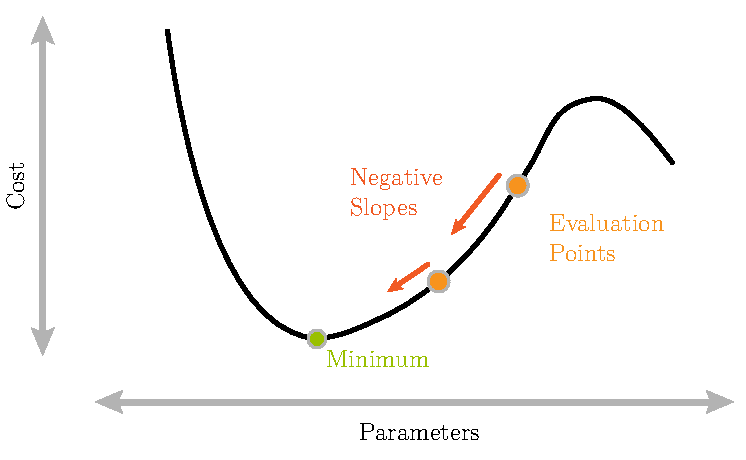
\includegraphics{images/gradient_descent.pdf}
	\caption[Schematic of gradient descent]{Schematic of gradient descent. Cost is evaluated, its negative gradients are computed and the parameters are moved along this direction until the minimum is reached.}
	\label{fig:gradient-descent}
\end{figure}
Following this approach means for the whole network that the cost function is backpropagated layer by layer to the beginning of the network using partial derivatives and the chain rule.
When this is completed, it is known how the parameters are influencing the output and therefore how they need to be changed depending on their slope.

The goal of backpropagation is to compute the partial derivatives
\begin{subequations}
	\label{eq:backpropagation}
	\begin{align}
		\frac{\partial J}{\partial w^{[l]}_{jk}} &= \frac{1}{m_{\text{train}}} \sum_{i}^{m_{\text{train}}} \frac{\partial J^{(i)}}{\partial w^{[l]}_{jk}} \\
		\frac{\partial J}{\partial b^{[l]}_j} &= \frac{1}{m_{\text{train}}} \sum_{i}^{m_{\text{train}}} \frac{\partial J^{(i)}}{\partial b^{[l]}_j}
	\end{align}
\end{subequations}
of the cost function w.r.t. the parameters by averaging the partial derivatives of cost functions of $m_{\text{train}}$ samples from the training set that were passed through the network.
These $m_{\text{train}}$ samples build a so-called batch in this context.
\figref{fig:backpropagation-influences} recaps the data flow in a neuron in the last layer.
By checking stepwise how a parameter directly influences a subsequent one, \eqref{eq:backpropagation} can be written as
\begin{subequations}
	\label{eq:backpropagation-last}
	\begin{align}
		\frac{\partial J}{\partial w^{[L]}_{jk}} &= \frac{\partial z^{[L]}_j}{\partial w^{[L]}_{jk}} \frac{\partial a^{[L]}_{j}}{\partial z^{[L]}_{j}} \frac{\partial J}{\partial a^{[L]}_{j}} \\
		\frac{\partial J}{\partial b^{[L]}_{j}} &= \frac{\partial z^{[L]}_j}{\partial b^{[L]}_{j}} \frac{\partial a^{[L]}_{j}}{\partial z^{[L]}_{j}} \frac{\partial J}{\partial a^{[L]}_{j}}
	\end{align}
\end{subequations}
for the last layer.
How much the activations of the second to last layer influence the cost function is expressed by
\begin{equation}
	\label{eq:backpropagation-activations-last}
	\frac{\partial J}{\partial a^{[L-1]}_{k}} = \sum_{j=1}^{n_y} \frac{\partial z^{[L]}_j}{\partial a^{[L-1]}_{k}} \frac{\partial a^{[L]}_{j}}{\partial z^{[L]}_{j}} \frac{\partial J}{\partial a^{[L]}_{j}}
\end{equation}
where all weighted sums and activations of the output layer are considered.
This needs to be done because layers are fully connected and the activation of one neuron influences every neuron in the next layer.
Especially in the last layer, the activation of one neuron in the second to last layer influences directly the activations of all neurons in the last layer.
Those are directly related to the cost, which is computed by comparing them with the ground-truth values.
Hence, the influences of the activations of the neurons in the second to last layer need to be summed up.
\begin{figure}
	\centering
	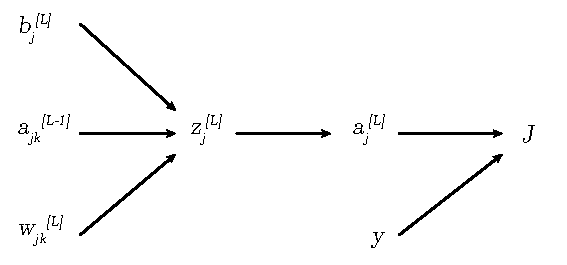
\includegraphics[]{images/backpropagation_influences.pdf}
	\caption[Data flow in a last-layer neuron for backpropagation]{Data flow in a last-layer neuron for backpropagation}
	\label{fig:backpropagation-influences}
\end{figure}
Once \eqref{eq:backpropagation-activations-last} is calculated for the second to last layer, this process can be repeated for all the weights and biases feeding into that layer.
This goes on layer for layer until the first one is reached.
In general,
\begin{equation}
	\label{eq:backpropagation-neuron-error}
	\delta^{[l]}_j = \frac{\partial J}{\partial a^{[l]}_j} \frac{\partial a^{[l]}_{j}}{\partial z^{[l]}_{j}}
\end{equation}
defines the error of the $j$-th neuron in the $l$-th layer.
Combining \eqref{eq:backpropagation-last} and \eqref{eq:backpropagation-neuron-error} yields
\begin{subequations}
	\label{eq:backpropagation-general}
	\begin{align}
		\frac{\partial J}{\partial w^{[l]}_{jk}} &= \frac{\partial z^{[l]}_j}{\partial w^{[l]}_{jk}} \frac{\partial a^{[l]}_{j}} {\partial z^{[l]}_{j}} \frac{\partial J}{\partial a^{[l]}_j} = \frac{\partial z^{[l]}_j}{\partial w^{[l]}_{jk}} \delta^{[l]}_j \\
		\frac{\partial J}{\partial b^{[l]}_{j}} &= \frac{\partial z^{[l]}_j}{\partial b^{[l]}_{j}} \frac{\partial a^{[l]}_{j}} {\partial z^{[l]}_{j}} \frac{\partial J}{\partial a^{[l]}_j} = \frac{\partial z^{[l]}_j}{\partial b^{[l]}_{j}} \delta^{[l]}_j
	\end{align}
\end{subequations}
as the general expressions for backpropagation where
\begin{subequations}
	\begin{align}
		\frac{\partial z^{[l]}_j}{\partial w^{[l]}_{jk}} &= a^{[l-1]}_j \\
		\frac{\partial z^{[l]}_j}{\partial b^{[l]}_j} &= 1 \\
		\frac{\partial a^{[l]}_{j}}{\partial z^{[l]}_{j}} &= \phi'(z^{[l]}_j)
	\end{align}
\end{subequations}
are the derivatives.
Summarizing the gradients of the cost function yields the compact representation
\begin{equation}
	\label{eq:cost-gradient}
	\nabla \vec{J} =
	\begin{pmatrix}
		\frac{\partial J}{\vec{W^{[1]}}} &
		\frac{\partial J}{\vec{b^{[1]}}} &
		\frac{\partial J}{\vec{W^{[2]}}} &
		\frac{\partial J}{\vec{b^{[2]}}} &
		\cdots &
		\frac{\partial J}{\vec{W^{[L]}}} &
		\frac{\partial J}{\vec{b^{[L]}}}
	\end{pmatrix}^T
\end{equation}
containing the influences of all parameters.
Each element points into its direction of steepest ascent with a magnitude.
Hence, each gradient is inverted for pointing into its direction of steepest descent for finding a minimum.
Along each direction, depending on its magnitude each parameter is changed.
This can be expressed by
\begin{subequations}
	\label{eq:learning-rate}
	\begin{align}
		w^{[l]}_{jk}(\tau + 1) &= w^{[l]}_{jk}(\tau) - \gamma \nabla \vec{J}(w^{[l]}_{jk}(\tau)) \\
		b^{[l]}_j(\tau + 1) &= b^{[l]}_j(\tau) - \gamma \nabla \vec{J}(b^{[l]}_j(\tau))
	\end{align}
\end{subequations}
where the hyperparameter $\gamma$ is the learning rate and $\tau$ the iteration step.
This update procedure is done for every batch that is passed through the network.
The updates resulting from a batch are called an iteration.
This is repeated for the whole training set, which is called an epoch.
The objective of the learning rate is to control how much the parameters are adjusted.
The smaller it is, the slower the parameters are moving along the graph to the minimum.
On its way, the slope steadily gets smaller which intensifies this effect.
A similar effect arises by moving over plateaus.
Surely, the minimum will be found more exactly than with a large learning rate, but it would make learning really slow.
However, a large learning rate can steadily overshoot the minimum leading to no convergence.
These effects are roughly exemplified in \figref{fig:learning-rate}.
Thus, a trade-off must be found or an adaption of the learning rate to certain circumstances like the magnitude of the slope is necessary.
\begin{figure}
	\centering
	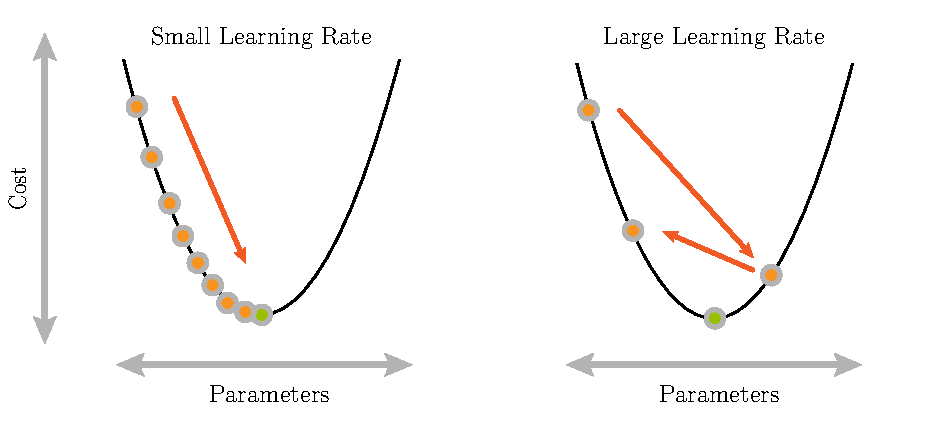
\includegraphics[]{images/gradient_descent_learning_rate.pdf}
	\caption[Comparison of learning rates]{Comparison of learning rates. A small learning rate finds the minimum slowly but more exactly than a high learning rate. However, the latter tends to overshoot the minimum. This is roughly exemplified.}
	\label{fig:learning-rate}
\end{figure}
According to \textit{Bengio} \cite{DBLP:journals/corr/abs-1206-5533} a traditional default value for the learning rate is $\gamma_0 = 0.1$ or $\gamma_0 = 0.01$ for standard multilayer neural networks.
However, it remains a hyperparameter that is problem-specific, hence, only guidelines can be provided.
One of them is, that the learning rate should be greater than $10^{-6}$ and less than $1.0$.
Another approach is decaying the initial learning rate either linearly or exponentially until iteration $\tau$ and then leaving it constant \cite{Goodfellow-et-al-2016}.
The underlying idea is to move quickly to close proximity to the minimum and then carefully to it.
Another common approach is an exponential decay like
\begin{equation}
	\gamma(\tau) = \gamma_0 \exp(-\lambda\tau)
\end{equation}
where $\gamma_0$ is the initial learning rate, $\lambda$ a factor and $\tau$ the iteration step.
The concept of changing the learning rate over time is called learning rate schedule. Its values are arbitrary and do not inevitably need to be results of a decay but can be fixed values that are active depending on the time step $\tau$, for example.

Due to the number of parameters and the use of hidden layers, cost functions are highly dimensional and neither convex nor concave.
An explanation for the latter is, that several combinations of parameters can result in the same loss value.
Hence, there are several local minima in the cost function.
According to \textit{Choromanska et al.} \cite{DBLP:journals/corr/ChoromanskaHMAL14} almost all local minima have very similar function values to the global minimum.
Hence, finding a local one is sufficient.
Having neither a convex nor concave cost function, the function probably has saddle points.
These points are no optimum but have a gradient of $\nabla \vec{J} = \vec{0}$.
The types of critical points are shown in \figref{fig:critical-points}.
\begin{figure}
	\centering
	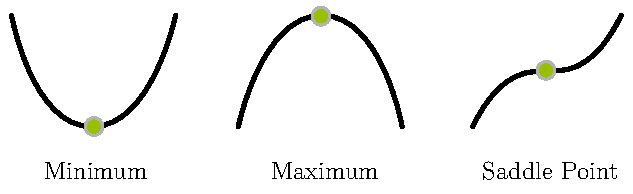
\includegraphics[]{images/gradient_descent_types.pdf}
	\caption{Types of critical points}
	\label{fig:critical-points}
\end{figure}
With this gradient the algorithm would get stuck.
Hence, adding some noise to \eqref{eq:learning-rate} yields
\begin{subequations}
	\begin{align}
		w^{[l]}_{jk} &:= w^{[l]}_{jk} - \gamma \nabla \vec{J}(w^{[l]}_{jk}) + \vec{\varepsilon}(w^{[l]}_{jk}) \\
		b^{[l]}_j &:= b^{[l]}_j - \gamma \nabla \vec{J}(b^{[l]}_j) + \vec{\varepsilon}(b^{[l]}_j)
	\end{align}
\end{subequations}
where $\vec{\varepsilon}$ is a noise vector with mean 0.
Because saddle points are very unstable, adding some noise helps to overcome them.
\subsubsection{Adam: Adaptive Moment Estimation}
\label{sec:training-adam}
Learning rate schedules have the problems of defining their parameters in advance and applying the same learning rate to every weight and bias.
Hence, the RMSProp (Root Mean Square Propagation) optimizer was developed\cite{Tieleman2012}.
Its objective is illustrated in \figref{fig:rmsprop}.
The ellipses represent contour lines.
The orange line visualizes the process of gradient descent.
Using it can result in parameters oscillating in one direction while making progress in another one moving to the minimum.
The objective of RMSProp, represented by the blue line, tries to dampen the oscillations by slowing down learning of the responsible parameter and fasten up the other one.
Hence, it can use a larger learning rate and reaches the minimum more quickly.
\begin{figure}
	\centering
	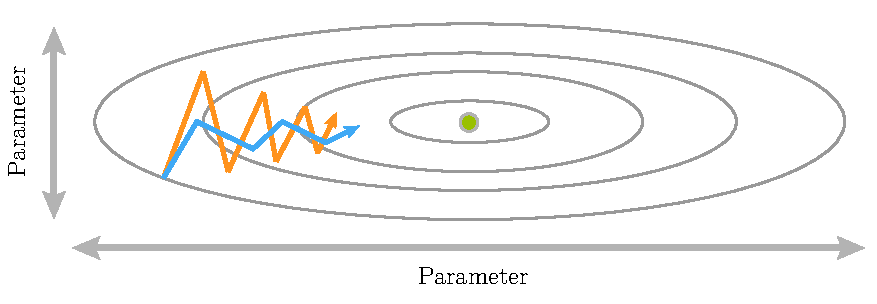
\includegraphics[]{images/rmsprop.pdf}
	\caption[Process of gradient descent and RMSProp]{Process of gradient descent and RMSProp using contour lines. The orange line illustrates the process of gradient descent. It oscillates and moves slowly to the minimum. The blue line shows the process of the RMSProp algorithm. While one parameter changes slower the other one changes faster. Hence, it dampens oscillations and moves faster to the minimum.}
	\label{fig:rmsprop}
\end{figure}
RMSProp adapts a learning rate to each of the parameters.
Furthermore, it divides the learning rate for a parameter by a weighted running average of the magnitudes of its previous gradients.
The weighted running average is calculated by
\begin{subequations}
	\label{eq:adam-second-momentum}
	\begin{align}
		v(w^{[l]}_{jk}, \tau) &= \beta_2 v(w^{[l]}_{jk}, \tau - 1) + (1-\beta_2) (\nabla \vec{J}(w^{[l]}_{jk}))^2 \\
		v(b^{[l]}_{j}, \tau) &= \beta_2 v(b^{[l]}_{j}, \tau - 1) + (1-\beta_2) (\nabla \vec{J}(b^{[l]}_{j}))^2
	\end{align}
\end{subequations}
where hyperparameter $\beta_2$ is the forgetting factor.
As a value, its author suggests $\beta_2 = 0.9$.
The subscript $2$ is for later purposes and could be omitted for now.
The squaring operation is done element-wise.
So this expression adds kind of inertia to the update procedure dampening oscillations and building up speed on flat surfaces.
Finally, the parameters are updated by
\begin{subequations}
	\begin{align}
		w^{[l]}_{jk} &:= w^{[l]}_{jk} - \frac{\gamma}{\sqrt{v(w^{[l]}_{jk}, \tau)}} \nabla \vec{J}(w^{[l]}_{jk}) \\
		b^{[l]}_{j} &:= b^{[l]}_{j} - \frac{\gamma}{\sqrt{v(b^{[l]}_{j}, \tau)}} \nabla \vec{J}(b^{[l]}_{j})
	\end{align}
\end{subequations}
using the weighted moving average just calculated.
Let's say the horizontal parameter is $w_1$ and the vertical one $w_2$ referring to \figref{fig:rmsprop}.
Due to the oscillations, the gradient $\nabla \vec{J}(w_2)$ is much larger than $\nabla \vec{J}(w_1)$.
Hence, $v_2$ is larger than $v_1$ resulting in a smaller update for $w_2$ and a larger one for $w_1$.
This yields a more direct moving to the minimum.
However, this approach does not make it easier to configure the learning rate as the step size is independent of it.
Though, it improves the speed of the optimization process because a better set of weights is discovered in fewer training steps than with pure gradient descent.
The Adam (Adaptive Moment Estimation) optimization is an update to the RMSProp algorithm by adding a momentum
\begin{subequations}
	\label{eq:adam-first-momentum}
	\begin{align}
		m(w^{[l]}_{jk},\tau) &= \beta_1 m(\tau -1) + (1- \beta_1) \frac{\partial J}{\partial w^{[l]}_{jk}} \\
		m(b^{[l]}_{j},\tau) &= \beta_1 m(\tau -1) + (1- \beta_1) \frac{\partial J}{\partial b^{[l]}_{j}}
	\end{align}
\end{subequations}
for each parameter using a weighted average of the latest gradients\cite{DBLP:journals/corr/KingmaB14} where $\beta_1$ is the forgetting factor.
This momentum can be imagined as a ball in a bowl-shaped cost function rolling downwards and building up speed depending on the gradients.
The hyperparameter $\beta_1$ represents friction.
This approach can be summarized by using running averages of both the gradients and the second moments of the gradients.
Due to the initialization $\vec{v} = \vec{0}$ and $\vec{m} = \vec{0}$ these values are biased towards zero, especially during the first few iterations.
A correction is desirable because the first and second moments are only estimations.
In general, an estimation should equal the parameter that is tried to be estimated.
Hence, the property
\begin{subequations}
	\begin{align}
		E[m] &= E[g]\\
		E[v] &= E[g^2]
	\end{align}
\end{subequations}
needs to be fulfilled, where $E[\cdot]$ represents the expectation of a variable.
These properties only hold true, if unbiased estimators are used.
Hence, the corrected values are expressed by
\begin{subequations}
	\label{eq:adam-corrected}
	\begin{align}
	\hat{m}(w^{[l]}_{jk}, \tau) &= \frac{m(w^{[l]}_{jk},\tau)}{1-\beta_1^\tau} \\
	\hat{m}(b^{[l]}_{j}, \tau) &= \frac{m(b^{[l]}_{j},\tau)}{1-\beta_1^\tau} \\
	\hat{v}(w^{[l]}_{jk}, \tau) &= \frac{v(w^{[l]}_{jk}, \tau)}{1-\beta_2^\tau} \\
	\hat{v}(b^{[l]}_{j}, \tau) &= \frac{v(b^{[l]}_{j}, \tau)}{1-\beta_2^\tau}
	\end{align}
\end{subequations}
using the expression from before.
Finally,
\begin{subequations}
	\label{eq:adam-update}
	\begin{align}
		w^{[l]}_{jk} := w^{[l]}_{jk}-\gamma \frac{\hat{m}(w^{[l]}_{jk})}{\sqrt{\hat{v}(w^{[l]}_{jk})} + \epsilon} \\
		b^{[l]}_{j} := b^{[l]}_{j}-\gamma \frac{\hat{m}(b^{[l]}_{j})}{\sqrt{\hat{v}(b^{[l]}_{j})} + \epsilon}
	\end{align}
\end{subequations}
updates the parameters, where $\epsilon$ is a small constant for preventing a division by zero.
As for other optimization algorithms the learning rate $\gamma$ needs to be tuned.
The remaining hyperparameters are recommended by \textit{Kingma et al.} to be $\beta_1 = 0.9$, $\beta_2 = 0.999$ and $\epsilon = 10^{-8}$.
However, the latter has no big impact on the optimization.